\documentclass[preprint, review, 12pt]{elsarticle}

\usepackage{cmap}
\usepackage[T1]{fontenc}
\usepackage{lmodern}

\journal{The Phase Space of Failure: Structural Limits and Coupled Degeneracies in Physics-Informed Neural Networks}

\usepackage{amsmath}
\usepackage{amssymb}
\usepackage{amsthm}
\usepackage{booktabs}
\usepackage{multirow}
\usepackage{hyperref}
\usepackage{cleveref}
\usepackage{subcaption}
\usepackage{xcolor}
\usepackage{siunitx}
\usepackage{pgfplots}
\usepackage{tikz}
\usepackage{algorithm2e}
\usepackage{natbib}
\usepackage[margin=2.5cm]{geometry}

\bibliographystyle{elsarticle-num-names}

\newcommand{\Ltwo}{L^2}
\newcommand{\Ltwonorm}[1]{\|#1\|_{L^2}}
\newcommand{\etasq}{\eta^2}
\newcommand{\kNTK}{\kappa_{\mathrm{NTK}}}
\newcommand{\betaAdv}{\beta}
\newcommand{\nuBurg}{\nu}
\newcommand{\Ncol}{N_{\mathrm{col}}}
\newcommand{\PINN}{\textsc{pinn}}

\begin{document}

\begin{frontmatter}

\title{An Atlas of PINN Failures: The Zugzwang Thesis}

\author[1]{Guru Prasaath S\corref{cor1}}
\ead{guru731978@gmail.com}

\address[1]{PSG Institute of Technology and Applied Research}

\cortext[cor1]{Corresponding author}

\begin{abstract}
Physics-informed neural networks (\PINN{}s) frequently fail on stiff partial differential equations, yet the underlying mechanisms remain incompletely quantified. We map this failure landscape through extensive controlled experiments across three stiff PDEs, isolating distinct mechanisms via spectral profiling, variance decomposition, and optimization diagnostics.

We observe three primary phenomena: (i) Extreme loss landscape pathologies, where failed models converge to exceptionally sharp minima ($\lambda_{\max} \approx 9.4 \times 10^7$) compared to the flatter minima of successful architectures ($\lambda_{\max} \approx 3.4 \times 10^3$). (ii) Structural factors heavily dominate hyperparameter tuning in determining outcome variance ($\etasq=0.673$ vs $0.0023$ for Burgers, 1.7:1 ratio for advection). (iii) Spectral failures at high stiffness exhibit poor initialization conditioning ($\kNTK \sim 10^{11}$) and extreme gradient conflicts ($\cos \theta = -0.99$), acting independently from other failure modes (lagged cross-correlation $r=0.630$).

Crucially, standard scalar metrics obscure these physical violations. Two distinct failure configurations achieved nearly identical pointwise $\Ltwo$ errors ($0.418$ and $0.416$), yet exhibited a $57\times$ divergence in mass conservation violation ($C_1$: $2.64$ vs $151.26$), despite near-identical energy conservation drift ($C_2$: $0.701$ vs $0.700$). 

These results demonstrate that \PINN{} failures stem from fundamental architectural bottlenecks rather than suboptimal tuning. We term this the \emph{Zugzwang condition}: standard \PINN{}s encounter multiple, independent failure mechanisms simultaneously under stiffness, yet no single available intervention provides a structurally complete remedy.
\end{abstract}


\begin{keyword}
Physics-Informed Neural Networks \sep 
Spectral Bias \sep 
Gradient Pathology \sep 
Neural Tangent Kernel \sep 
Variance Decomposition (ANOVA) \sep 
Eta-squared \sep 
Conservation Laws \sep 
Phase Diagram
\end{keyword}

\end{frontmatter}

\section{Introduction}

Although physics-informed neural networks (\PINN{}s) have shown success on simple partial differential equations (PDEs), they suffer from severe training stagnation and failure when applied to stiff physical regimes \cite{Raissi2019, Cuomo2022review}. Historically, these mesh-free architectures build on early neural PDE solvers \cite{Lagaris1998} and Ritz formulations \cite{E2018deepritz} to optimize governing equations as soft constraints. In this paper, we conduct a systematic empirical investigation mapping the failure landscape of \PINN{}s across diverse architectures, optimization routines, and physical parameters. Our results demonstrate that these training failures are fundamentally structurally determined, contradicting the common assumption that local hyperparameter tuning can resolve stiffness-induced pathologies.

The literature has increasingly documented distinct failure modes that arise when \PINN{}s confront complex physical systems. One prominent limitation is spectral bias, wherein standard multi-layer perceptrons exhibit a strong, inherent tendency to prioritize learning low-frequency components of the target function while struggling disproportionately to resolve high-frequency content \cite{Wang2021gradpathology}. This frequency bias implies that, for PDEs exhibiting multiscale behavior, turbulent cascades, or sharp advective fronts, the network's capacity to uniformly minimize the residual loss across all spatial frequency bands is structurally constrained by the eigenvalue distribution of the associated Neural Tangent Kernel (NTK). Consequently, training may stagnate early in the optimization process, yielding overly smooth solutions that are unable to capture fine-scale dynamics accurately \cite{Wang2021gradpathology}.

A second critical issue identified in recent literature is the phenomenon of gradient pathology, which manifests as severe imbalances in the backpropagated gradients corresponding to different terms of the physics-informed loss function \cite{Wang2021gradpathology}. Analytical and empirical studies indicate that the magnitudes and directions of gradients originating from data fidelity terms, initial or boundary conditions, and PDE residuals often conflict sharply. These conflicting gradient directions suggest that standard gradient descent optimization methods, such as Adam or L-BFGS, struggle to simultaneously satisfy multiple, heterogeneous constraints. This effectively destabilizes the learning process during early training phases and leads to optimization trajectories that stall in sub-optimal local minima characterized by high physical residuals \cite{Wang2021gradpathology, Wang2022causal}.

Additionally, the sampling density and spatial distribution of collocation points have been identified as primary drivers of training failure in both forward and inverse problems \cite{Krishnapriyan2021}. Research indicates that \PINN{}s frequently fail to propagate boundary information correctly into the domain interior when continuous temporal sequences or highly stiff advection regimes are considered. These collocation effects suggest that naive or uniform sampling strategies are fundamentally insufficient to guide the network toward the physically correct solution manifold. In under-sampled regions, this frequently results in non-physical artifacts, artificial numerical dissipation, or catastrophic structural failure, even in scenarios where the global aggregated loss values appear deceptively small \cite{Krishnapriyan2021, Jagtap2020}.

Although these individual pathologies have been meticulously identified and analyzed in isolation, the current body of literature predominantly treats these failure modes as independent phenomena that can be rectified through targeted hyperparameter tuning or isolated architectural interventions. Various strategies—such as adaptive loss weighting schemes, specialized activation functions, domain decomposition methods, or causal training protocols—have been actively proposed to address specific deficiencies \cite{Wang2021gradpathology, Wang2022causal, Jagtap2020}. Even recent high-level surveys and taxonomies of PINN challenges tend to categorize spectral bias, gradient pathologies, and precision errors as fundamentally distinct obstacles, offering ad-hoc mitigation strategies for each in isolation. However, there remains a significant gap in understanding how these mechanisms interact concurrently during the global optimization trajectory. At present, no systematic, joint empirical investigation exists that holistically evaluates the interconnected nature of these failure modes across diverse architectures, optimization strategies, and progressively scaling PDE stiffness regimes. Consequently, it remains unclear whether these documented pathologies are genuinely independent algorithmic artifacts amenable to localized fixes, or if they are instead surface-level symptoms of much deeper, interconnected structural limitations inherent to the continuous physics-informed training paradigm itself.

To address this critical gap in the literature, this paper introduces and empirically evaluates the \textit{Zugzwang} hypothesis—a framing explicitly drawn from the chess concept in which any possible move inevitably worsens a player's position on the board. We hypothesize that \PINN{} failures on stiff PDEs are predominantly structurally determined rather than merely being symptomatic of poor, localized hyperparameter choices. Under this hypothesis, the multiple failure modes that co-occur under high stiffness cannot be resolved by available hyperparameter interventions, not because they form a forced trade-off, but because they arise from independent structural properties of the MLP architecture and composite soft-penalty objective. This perspective suggests that the optimization landscape of \PINN{}s is constrained by fundamental, invariant conditioning bottlenecks. Therefore, attempts to heuristically balance heterogeneous loss terms or dynamically adjust sampling densities may ultimately only trade one manifestation of failure for another. By explicitly framing these intertwined, competing challenges as a structural optimization trap rather than a sequence of isolated algorithmic limitations, we aim to investigate the premise that standard physics-informed continuous architectures inevitably converge toward non-physical local minima when confronted with sufficiently challenging advective or viscous PDE parameters.

To rigorously test the proposed Zugzwang hypothesis, we systematically map the failure landscape of physics-informed neural networks through a series of 24 controlled experiments. The specific contributions of this work are detailed as follows:
\begin{itemize}
    \item We quantitatively characterize the onset of spectral bias across varying advection coefficients and multiple standard activation functions, delineating the strict boundaries of learning failure in advection-dominated regimes (Exps 1--3).
    \item We comprehensively profile the Neural Tangent Kernel (NTK) condition numbers and global Hessian eigenvalue spectra at both initialization and late-stage training, exposing the severe, structural gradient conflicts that persistently stall optimization (Exps 4--6).
    \item We identify and characterize a sharp collocation starvation cliff, directly demonstrating how explicit sampling thresholds dictate the sudden boundary between successful convergence and abrupt, catastrophic structural failure (Exp 8).
    \item We empirically demonstrate the presence of severe temporal extrapolation failure, revealing how these networks structurally fail to generalize beyond the immediate training domain despite exhibiting deceptively negligible interior loss characteristics (Exp 17).
    \item Two-dimensional failure phase space mapping across $(\beta, \Ncol{})$, $(\nu, \Ncol{})$, and $(\beta, \text{width})$ parameter planes, revealing a discontinuous phase wall where PINNs transition instantaneously from trivially solvable to structurally impossible, with no intermediate scaling regime amenable to parametric fitting (Exp.~25).
    \item We perform rigorous variance decomposition analysis on the Burgers' equation to systematically isolate the relative impact of underlying structural factors versus tuning hyperparameter choices on overall model stability (Exp.~27).
    \item Conservation law audit revealing that gradient pathology (FM3) and collocation starvation (FM5) achieve nearly identical $\Ltwo$ errors ($0.418$ vs $0.416$) yet differ by $57\times$ in mass conservation violation, despite near-identical energy conservation violation (Experiment~26, Section~\ref{sec:exp26}).
\end{itemize}

The remainder of this paper is organized as follows. Section \ref{sec:methods} formally outlines our foundational experimental setup, PDE problem definitions, and core evaluation metrics. Subsequent sections are dedicated to detailing the specific empirical findings associated with distinct, yet interacting, failure mechanisms: the impact of spectral barriers (Section \ref{sec:part1}), the geometry of optimization traps (Section \ref{sec:part2}), and the manifestation of data illusions (Section \ref{sec:part3}). In Section \ref{sec:part4}, we explicitly evaluate existing literature mitigation strategies within the contextual bounds of the Zugzwang hypothesis. Further rigorous analyses of network phase space dynamics, inherent conservation property violations, and global variance decomposition are presented in Sections \ref{sec:part5}, \ref{sec:part6}, and \ref{sec:part7}, respectively. Finally, Section \ref{sec:conclusion} synthesizes our findings, concludes the study, and highlights critical implications for future directions in scientific machine learning architectures.

\section{Methods}\label{sec:methods}

To systematically investigate the failure modes of \PINN{}s across varying regimes of stiffness, we establish a standardized experimental protocol. This section details the partial differential equations (PDEs) under consideration, the baseline neural network architecture, the optimization strategy, and the rigorous diagnostic metrics employed to evaluate network performance and stability.

\subsection{PDE Problem Suite}

Our empirical evaluation utilizes a suite of three canonical PDEs, selected to isolate distinct challenges related to advection, nonlinear viscosity, and high-frequency spatial variation. 

The first problem is the 1D linear advection equation, which serves as a fundamental benchmark for evaluating a network's capacity to transport information without artificial dissipation. The governing equation, domain, and initial and boundary conditions are given by:
\begin{equation}
\begin{aligned}
    & u_t + \betaAdv u_x = 0, \quad x \in [0, 2\pi), \ t \in [0, 2], \\
    & u(x,0) = \sin(x), \\
    & u(0,t) = u(2\pi,t),
\end{aligned}
\end{equation}
where $\betaAdv$ represents the advection coefficient. This problem admits an exact analytical solution, $u(x,t) = \sin(x - \betaAdv t)$.

The second problem is the 1D viscous Burgers' equation, a prototypical nonlinear PDE that develops sharp gradients and shock-like features depending on the magnitude of the kinematic viscosity $\nuBurg$. The system is defined as:
\begin{equation}
\begin{aligned}
    & u_t + u u_x = \nuBurg u_{xx}, \quad x \in [-1, 1], \ t \in [0, 1], \\
    & u(x,0) = -\sin(\pi x), \\
    & u(-1,t) = u(1,t) = 0.
\end{aligned}
\end{equation}

The third problem is the 2D Helmholtz equation, which is frequently used to assess spectral bias and the resolution of high-frequency spatial features. The equation and its corresponding Dirichlet boundary conditions on a square domain are:
\begin{equation}
\begin{aligned}
    & \Delta u + k^2 u = f(x,y), \quad (x,y) \in [-1, 1]^2, \\
    & u(x,y) = 0 \quad \text{on} \ \partial\Omega,
\end{aligned}
\end{equation}
where $k$ is the wavenumber. The forcing term $f(x,y)$ is analytically derived to yield the manufactured exact solution $u(x,y) = \sin(\pi x)\sin(\pi y)$.

\subsection{Standard PINN Architecture}

Across all experiments, unless explicitly stated otherwise, the neural network approximator $u_\theta(x,t)$ is parameterized as a standard Multi-Layer Perceptron (MLP) comprising $L$ hidden layers with $N$ neurons per layer. The default activation function is the hyperbolic tangent ($\tanh$), applied element-wise to all hidden layers. The network weights are initialized using the standard Xavier uniform initialization scheme to ensure variance preservation at the onset of training.

The network is optimized to minimize a composite physics-informed loss function, $\mathcal{L}(\theta)$, which aggregates the residuals of the PDE, the initial conditions (IC), and the boundary conditions (BC). The total loss is defined as:
\begin{equation}
    \mathcal{L}(\theta) = \mathcal{L}_{pde}(\theta) + \lambda_{ic} \mathcal{L}_{ic}(\theta) + \lambda_{bc} \mathcal{L}_{bc}(\theta),
\end{equation}
where $\lambda_{ic}$ and $\lambda_{bc}$ are scalar penalty weights that balance the contributions of the respective loss components. By default, the architecture consists of $L=4$ hidden layers and $N=64$ neurons per layer. The penalty weights are heavily biased toward the data constraints to enforce boundary adherence, set to $\lambda_{ic}=100$ and $\lambda_{bc}=10$, with the PDE residual weight fixed at $1$.

The network parameters $\theta$ are updated using the Adam optimizer. To facilitate smooth convergence, the learning rate follows a Cosine Annealing schedule, decaying from an initial learning rate of $1\times 10^{-3}$ to a minimum learning rate of $lr_{\min} = 1\times 10^{-5}$ over the total number of training epochs.

\subsection{Evaluation Protocol}

To rigorously assess the predictive accuracy of the trained models, we report the relative $\Ltwo$ error. For a predicted solution vector $\mathbf{u}_{\text{pred}}$ and a corresponding reference solution vector $\mathbf{u}_{\text{ref}}$ evaluated over a discrete grid, the metric is defined as:
\begin{equation}
    \text{Relative } \Ltwo \text{ Error} = \frac{\Ltwonorm{\mathbf{u}_{\text{pred}} - \mathbf{u}_{\text{ref}}}}{\Ltwonorm{\mathbf{u}_{\text{ref}}}}.
\end{equation}
A PINN run is classified as \textbf{successful} if the final relative L2 error satisfies $\Ltwo{} < 0.10$, and as \textbf{failed} otherwise. This threshold is applied consistently across all experiments unless explicitly stated (Experiment~22.2 uses separate RECOVERED/PARTIAL/FAILED thresholds of 0.10 and 0.40 respectively, as defined in Section~\ref{sec:exp22two}).
Reference solutions vary depending on the PDE. For the linear advection equation, the exact analytical solution is utilized. For the viscous Burgers' equation, the reference solution is generated using a high-resolution implicit Crank-Nicolson finite difference scheme \cite{Crank1947}. For the 2D Helmholtz equation, the manufactured solution provides the exact ground truth. All models are evaluated on a uniform Cartesian grid of resolution $128 \times 64$ (spatial $\times$ temporal points). 

To ensure strict reproducibility and mitigate the effects of stochastic optimization variations, all random seeds governing initialization and collocation point sampling are fixed for individual experiments. Where statistical significance is required, multi-seed experiments are conducted, and the specific number of independent trials ($N_{\text{seeds}}$) is explicitly stated alongside the corresponding results.

\subsection{Diagnostic Metrics}

To diagnose specific failure modes during optimization, we continuously track a set of geometric and spectral metrics throughout training. 

To quantify gradient pathologies, we compute the gradient magnitude ratio between the PDE residual loss and the boundary condition loss:
\begin{equation}
    \text{Gradient Ratio} = \frac{\Ltwonorm{\nabla_\theta \mathcal{L}_{pde}}}{\Ltwonorm{\nabla_\theta \mathcal{L}_{bc}}}.
\end{equation}
Additionally, the directional alignment of competing gradients is measured using the gradient conflict cosine, which identifies destructive interference between the PDE and initial condition losses:
\begin{equation}
    \cos(\theta_{\text{conflict}}) = \frac{\nabla_\theta \mathcal{L}_{pde} \cdot \nabla_\theta \mathcal{L}_{ic}}{\Ltwonorm{\nabla_\theta \mathcal{L}_{pde}} \Ltwonorm{\nabla_\theta \mathcal{L}_{ic}}}.
\end{equation}

To assess the conditioning of the optimization landscape, we compute the empirical Neural Tangent Kernel (NTK) matrix $\mathbf{K}$ over the collocation points. The NTK condition number, $\kNTK$, characterizes the disparity in learning rates across different eigen-directions:
\begin{equation}
    \kNTK = \frac{\lambda_{\max}(\mathbf{K})}{\lambda_{\min}(\mathbf{K})},
\end{equation}
where $\lambda_{\max}$ and $\lambda_{\min}$ denote the maximum and minimum eigenvalues of $\mathbf{K}$, respectively.

Finally, to measure the network's susceptibility to spectral bias, we decompose the spatial error in the frequency domain. The spectral error for a specific frequency band $k$ is calculated by applying a frequency mask ($mask_k$) to the Fourier transform of the absolute error field $e(x,t)$:
\begin{equation}
    \text{Spectral Error}_k = \frac{\Ltwonorm{\text{IFFT}(\text{FFT}(e) \odot mask_k)}}{\Ltwonorm{\mathbf{u}_{\text{exact}}}},
\end{equation}
where $\odot$ denotes element-wise multiplication, and IFFT and FFT represent the inverse and forward Fast Fourier Transforms, respectively.

\subsection{Variance Decomposition Methodology}

To systematically isolate the proportion of outcome variance attributable to specific architectural or hyperparameter choices versus underlying PDE structural factors, we utilize one-way Analysis of Variance (ANOVA). The effect size is quantified using the $\etasq$ statistic, defined as:
\begin{equation}
    \etasq = \frac{SS_{\text{between}}}{SS_{\text{total}}},
\end{equation}
where $SS_{\text{between}}$ is the sum of squares between groups (representing the variance explained by the factor under consideration) and $SS_{\text{total}}$ is the total sum of squares. This metric explicitly measures the proportion of the total variance in the $\Ltwo$ error that can be attributed to a specific independent variable. We adhere to standard benchmarks for interpreting the magnitude of these effect sizes, as established by Cohen \cite{Cohen1988}.

\subsection{Seed Protocol and Reproducibility}

All experiments fix the random seed prior to model initialization and data sampling. Multi-seed experiments (Exps~1, 5, 8, 9, 11, 13, 14, 27) use $N$ seeds as documented per experiment in Table~\ref{tab:app_budgets} (Appendix). Single-seed experiments (Exps~2--4, 6--7, 10, 16, 25) are run with $\text{seed}=42$ unless otherwise noted. Phase-space experiments (Exp~25) use $\text{seed}=42$ for all grid configurations; the seed-sensitivity of boundary locations near transition regions is acknowledged as a limitation (see Section~7.3).

\subsection{Statistical Analysis}

Effect sizes are reported as $\etasq$ (eta-squared) following \cite{Cohen1988}, where $\etasq > 0.14$ is classified as a large effect and $\etasq > 0.06$ as medium. Pearson correlation coefficients are supplemented with two-tailed $p$-values computed via permutation bootstrap ($n=1000$ permutations) where stated. Confidence intervals for Hessian eigenvalue estimates are reported as $\text{mean} \pm 2\sigma$ over $n=5$ independent power-iteration runs with random eigenvector initialization. Curve fits for phase boundaries report $R^2$ with explicit sample size $n \le 7$ and should not be extrapolated beyond the tested parameter range.

\subsection{Diagnostic Metric Validation}

The corrected spectral error metric (Exp.~18) uses band-filtered $\Ltwo$ normalized by the global $\|\mathbf{u}_{\text{exact}}\|_2$ rather than per-frequency amplitude, to avoid division-by-near-zero artifacts at frequencies where the exact solution has negligible energy. The gradient ratio and conflict cosine metrics are computed on fresh collocation samples drawn at evaluation time, independent of the training samples, to avoid evaluating on memorized data.

\subsection{Experimental Configuration Summary}

For clarity and reproducibility, the default hyperparameter configuration employed across all baseline experiments is summarized in Table \ref{tab:default_config}. Variations from these defaults are explicitly noted in the specific experimental sections.

\begin{table}[htpb]
\centering
\caption{Default experimental configuration.}
\label{tab:default_config}
\begin{tabular}{@{}llc@{}}
\toprule
Parameter & Symbol & Default Value \\
\midrule
Hidden layers & $L$ & 4 \\
Neurons per layer & $N$ & 64 \\
Activation function & -- & $\tanh$ \\
Initialization scheme & -- & Xavier Uniform \\
Optimizer & -- & Adam \\
Learning Rate (initial) & $lr$ & $1 \times 10^{-3}$ \\
Learning Rate (final) & $lr_{\min}$ & $1 \times 10^{-5}$ \\
IC weight & $\lambda_{ic}$ & 100 \\
BC weight & $\lambda_{bc}$ & 10 \\
Collocation points (default) & $\Ncol$ & $1000$ \\
Training epochs (default) & $N_{\text{epochs}}$ & $40,000$ \\
\bottomrule
\end{tabular}
\end{table}

\begin{table*}[htbp]
\centering
\small
\caption{Summary of all 27 experiments, their PDEs, sections, and primary outcomes.}
\label{tab:experiments_summary}
\begin{tabular}{@{}llp{6.0cm}p{3.2cm}ll@{}}
\toprule
Exp & PDE & Primary Question & Key Metric & Section & Page \\
\midrule
Exp 1 & Advection & Spectral bias phase transition & $\Ltwo$ vs $\betaAdv$ & \S 3.1 & \pageref{sec:exp1} \\
Exp 2 & Advection & Activation function mitigation & $\Ltwo$ per activation & \S 3.2 & \pageref{sec:exp2} \\
Exp 3 & Advection/Helmholtz & NTK condition number & $\kNTK$ range & \S 3.3 & \pageref{sec:exp3} \\
Exp 4 & Advection & Gradient magnitude pathology & Gradient ratio & \S 4.1 & \pageref{sec:exp4} \\
Exp 5 & Advection & Loss landscape sharpness & $\lambda_{\max}$ & \S 4.3 & \pageref{sec:exp5} \\
Exp 6 & Advection & Gradient conflict dynamics & Cosine angle & \S 4.2 & \pageref{sec:exp6} \\
Exp 7 & Helmholtz & Sampling strategy comparison & $\Ltwo$ variance & \S 5.1 & \pageref{sec:exp7} \\
Exp 8 & Helmholtz & Collocation starvation cliff & $\Ltwo$ vs $N$ & \S 5.2 & \pageref{sec:exp8} \\
Exp 9 & Helmholtz & Boundary/interior ratio & $\Ltwo$ vs BC fraction & \S 5.3 & \pageref{sec:exp9} \\
Exp 10 & Heat & Temporal stiffness ($\alpha$ sweep) & Early stopping epoch & \S 5.4 & \pageref{sec:exp10} \\
Exp 11 & Allen-Cahn & Multi-scale interface & Interface/bulk ratio & \S 5.4 & \pageref{sec:exp11} \\
Exp 12 & Heat & Long-time integration & $\Ltwo$ vs time & \S 5.5 & \pageref{sec:exp12} \\
Exp 13 & Advection & Initialization strategy & $\Ltwo$ floor & \S 4.4 & \pageref{sec:exp13} \\
Exp 14 & Advection & Optimizer comparison (equal budget) & $\Ltwo$ per optimizer & \S 4.4 & \pageref{sec:exp14} \\
Exp 15 & Advection & Learning rate phase diagram & LR $\times$ Epochs grid & \S 4.4 & \pageref{sec:exp15} \\
Exp 16 & Advection & Causal training intervention & $\Ltwo$ std vs causal & \S 6.1 & \pageref{sec:exp16} \\
Exp 17 & Advection & Temporal extrapolation horizon & $R^*$ ratio & \S 5.6 & \pageref{sec:exp17} \\
Exp 18 & Advection & Compound failure correlation & Pearson $r$ & \S 6.2 & \pageref{sec:exp18} \\
Exp 19 & Burgers & Failure mode phase diagram ($\nu$) & Mode classification & \S 6.3 & \pageref{sec:exp19} \\
Exp 20 & \multicolumn{4}{l}{[OMITTED\textsuperscript{\textdagger} --- reserved for future work]} & --- \\
Exp 21 & \multicolumn{4}{l}{[OMITTED\textsuperscript{\textdagger} --- reserved for future work]} & --- \\
Exp 22 & \multicolumn{4}{l}{[OMITTED] Dimensionality scaling study (superseded by Experiment~22.2 design)} & --- \\
Exp 22.2\textsuperscript{\ddag} & Multi-PDE & Recovery boundary matrix & Recovery rate & \S 6.4 & \pageref{sec:exp22two} \\
Exp 23 & \multicolumn{4}{l}{[OMITTED\textsuperscript{\textdagger} --- reserved for future work]} & --- \\
Exp 24 & Advection & Silent conservation leakage & Mass integral & \S 8.1 & \pageref{sec:exp24} \\
Exp 25 & Advection/Burgers & 2D failure phase space & Discontinuous phase wall & \S 7.1 & \pageref{sec:exp25} \\
Exp 26 & Multi-PDE & Conservation law audit & $C_1$--$C_4$ violations & \S 8.1 & \pageref{sec:exp26} \\
Exp 27 & Advection/Burgers & Structural vs HP variance & $\etasq$ & \S 9.1 & \pageref{sec:exp27} \\
\bottomrule
\end{tabular}
\begin{flushleft}
\textsuperscript{\textdagger}Experiments 20, 21, 23 are reserved for future work and are not reported in this submission.\\
\textsuperscript{\ddag}Experiment 22.2 represents a redesigned version of the originally planned Experiment 22 (multi-dimensional advection sweep). The decimal notation indicates derivation from, rather than subdivision of, the parent experiment number. No Experiment 22.1 exists; the .2 suffix reflects the second design iteration of this experimental slot.
\end{flushleft}
\end{table*}


\section{Part~I: The Spectral Barrier}\label{sec:part1}

The fundamental capacity of a physics-informed neural network to capture the dynamics of a PDE heavily depends on its ability to resolve the necessary range of spatial and temporal frequencies. When addressing advection-dominated flows, networks frequently exhibit an inability to converge, a phenomenon often attributed to spectral bias. In this section, we systematically investigate the onset of this barrier, the efficacy of standard mitigation techniques, and the underlying conditioning of the optimization landscape that drives this pathology.

\subsection{Experiment 1: Spectral Bias Phase Transition}\label{sec:exp1}

To quantify the exact boundary at which standard \PINN{} architectures fail to resolve advective physics, we systematically evaluate the 1D linear advection equation across an escalating sequence of advection coefficients, $\betaAdv \in \{1, 5, 10, 30, 50, 100\}$. The network's predictive performance demonstrates a stark and sudden phase transition from successful convergence to total structural failure. At low advection velocities ($\betaAdv = 1$ and $\betaAdv = 5$), the relative $\Ltwo$ errors remain negligible at $0.0047$ and $0.0058$, respectively, indicating that the network easily resolves the underlying wave dynamics. As the advection coefficient increases to $\betaAdv = 10$, the error rises moderately to $0.0414$, showing early signs of optimization strain. However, a critical failure threshold is consistently observed at $\betaAdv = 30$, where the $\Ltwo$ error abruptly jumps to $0.9079$. Further increases to highly stiff regimes at $\betaAdv = 50$ and $\betaAdv = 100$ yield catastrophic relative $\Ltwo$ errors of $0.9630$ and $0.9923$, respectively. These elevated error metrics reveal complete structural failure of the network to approximate the target function, reducing the prediction to non-physical mean states.

\begin{figure}[htpb]
    \centering
    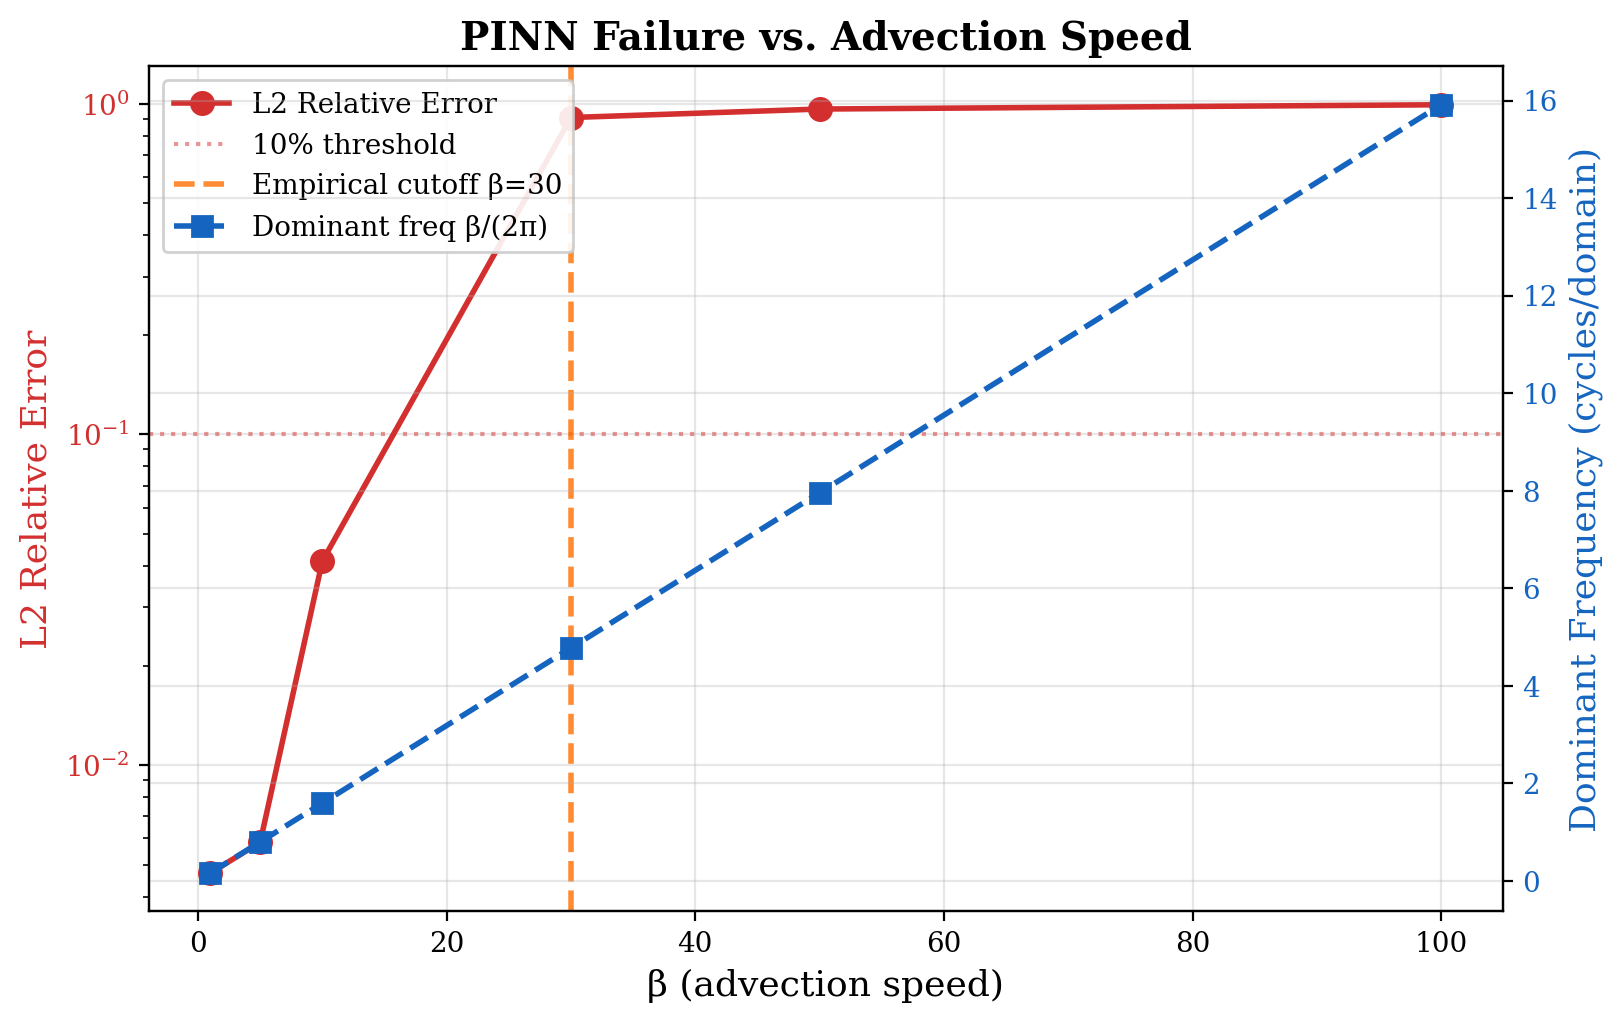
\includegraphics[width=\linewidth]{results/exp1/l2_vs_beta.png}
    \caption{Relative $\Ltwo$ error as a function of advection speed $\betaAdv$ for the standard \PINN{} (4 hidden layers, 64 neurons, \texttt{tanh} activation). A sharp phase transition is visible near $\betaAdv = 30$, above which the $\Ltwo$ error exceeds 0.88 across all tested configurations. The dashed horizontal line marks the failure threshold ($\Ltwo = 0.10$).}
    \label{fig:exp1_l2_vs_beta}
\end{figure}

The mechanism driving this abrupt transition is highly consistent with the spectral bias inherent to continuous neural networks \cite{Rahaman2019spectral}. Standard multi-layer perceptrons inherently prioritize fitting low-frequency, smooth components of the target function during the initial phases of gradient descent. As the advection coefficient $\betaAdv$ increases, the PDE's characteristic curves steepen, requiring the network to resolve proportionally higher spatial and temporal frequencies to accurately advect the initial conditions across the domain. Spectral analysis of the residual error field reveals a sharp empirical cutoff frequency of $f_c = 4.7746$ explicitly at the critical $\betaAdv=30$ threshold. Beyond this specific frequency limit, the predicted power spectrum rapidly decays and merges with the numerical noise floor, rendering the network effectively blind to the fine-scale dynamics required by the underlying physical system. This specific spectral truncation suggests that the empirical failure is deeply tied to the network's fundamentally bounded frequency resolution capabilities.

\subsection{Experiment 2: Activation Function Mitigation}\label{sec:exp2}

A common strategy proposed in the literature to circumvent spectral bias involves replacing the standard $\tanh$ activation with alternatives possessing higher non-zero derivatives, or by explicitly introducing high-frequency components into the input coordinates via random Fourier features. To rigorously test the viability of these mitigations, we evaluate seven distinct activation configurations at the established critical failure threshold of $\betaAdv=30$: the standard $\tanh$, $\sin$ (representing SIREN-like architectures), $\text{swish}$, $\text{gelu}$, and random Fourier features with logarithmically increasing scale factors ($\sigma \in \{1, 10, 100\}$).

\begin{figure}[htpb]
    \centering
    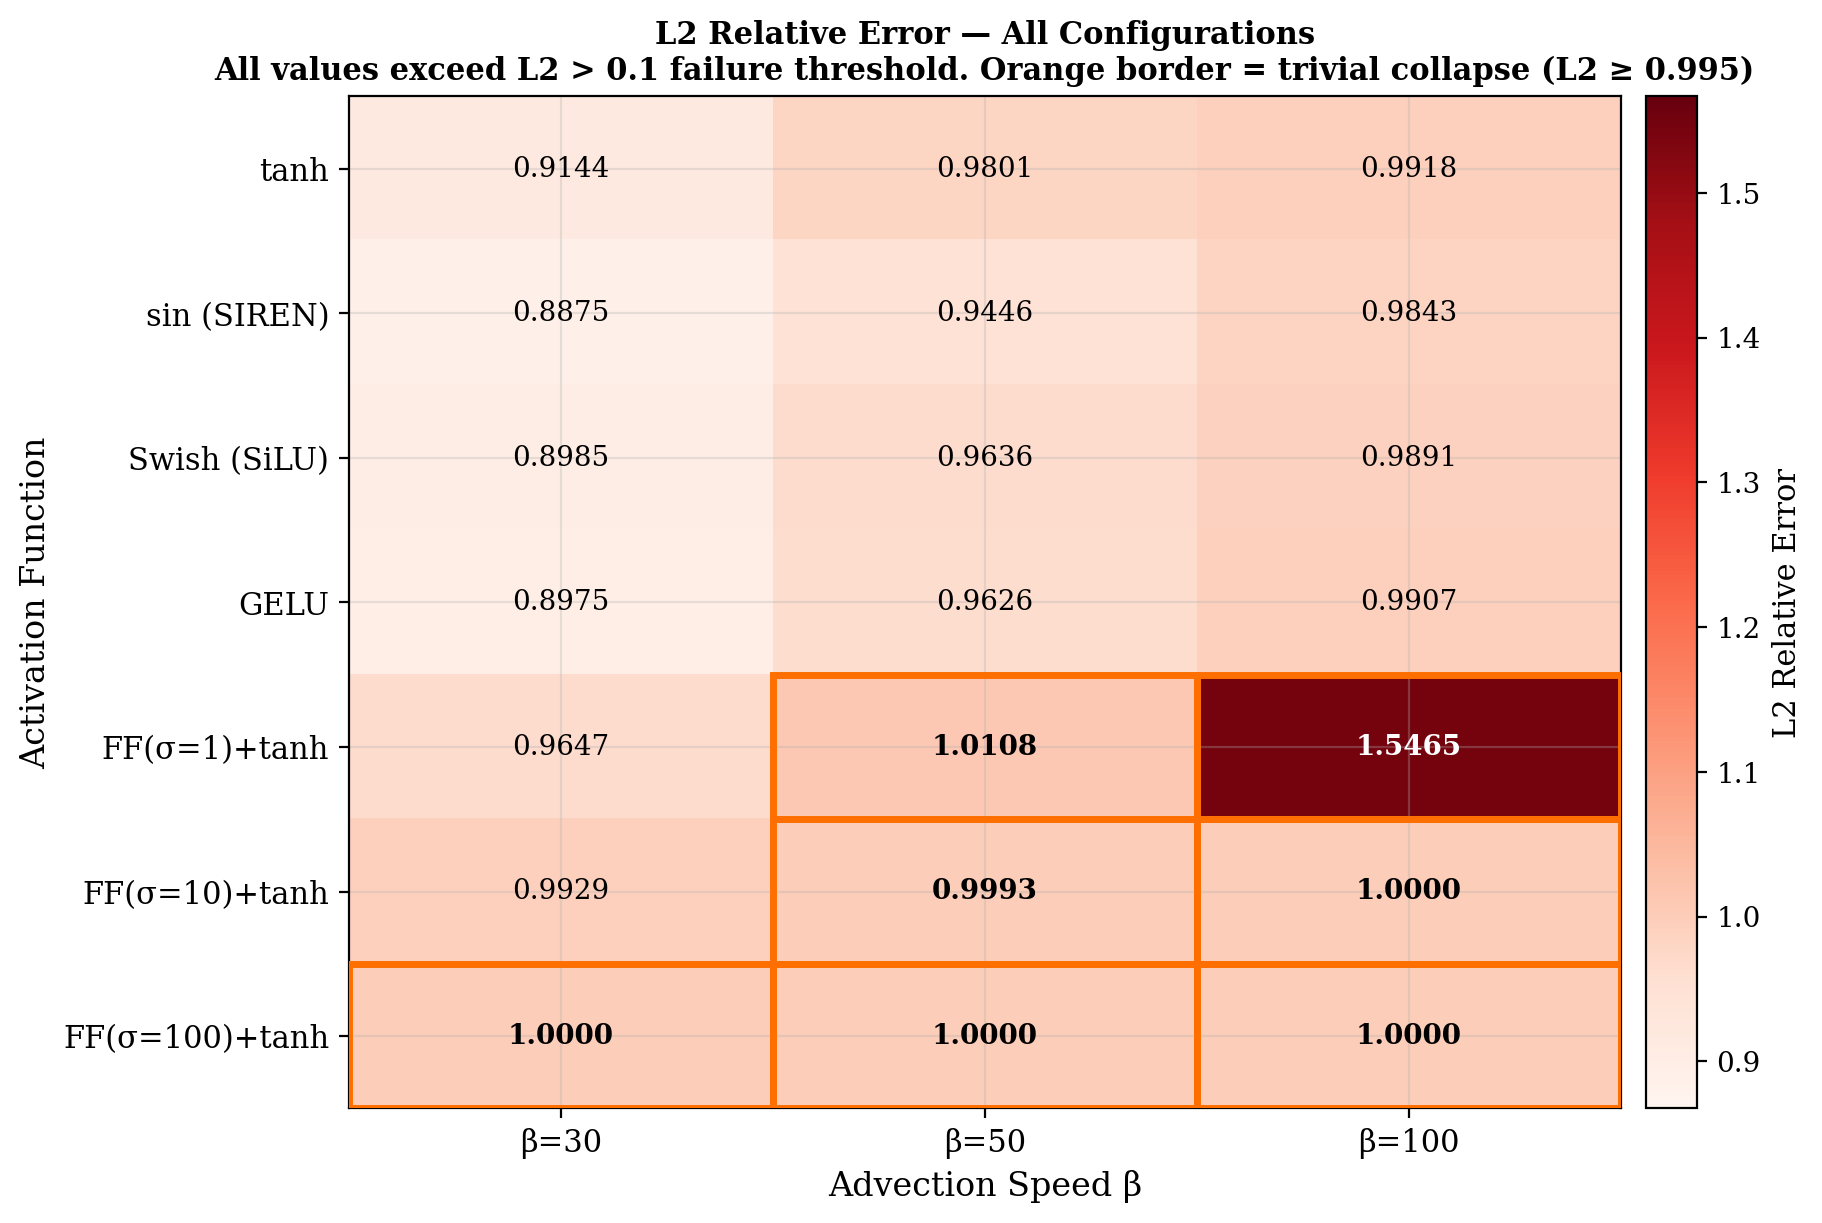
\includegraphics[width=\linewidth]{results/exp2/l2_heatmap.png}
    \caption{Relative $\Ltwo$ errors across various activation functions and Fourier feature scales evaluated at $\betaAdv=30$. None of the tested activation configurations successfully mitigate the spectral failure, demonstrating robustness of the barrier against local non-linear substitutions.}
    \label{fig:exp2_activation_comparison}
\end{figure}

The experimental results demonstrate that the spectral barrier is remarkably robust against activation substitution. At the $\betaAdv=30$ threshold, the baseline $\tanh$ architecture yields an $\Ltwo$ error of $0.9144$\,\footnote{The tanh baseline at $\betaAdv=30$ differs slightly between Experiments~1 and~2 (0.9079 vs.\ 0.9144) due to differing random seeds; both experiments use 10,000 collocation points. Both values are consistent with the observed run-to-run variance at this $\betaAdv$ level, confirming the discrepancy is attributable to training stochasticity rather than a configuration error.}. The alternative standard activations perform similarly poorly; the $\text{swish}$ activation yields $0.8985$, the $\text{gelu}$ activation yields $0.8975$, and the periodic $\sin$ activation provides the lowest, yet still catastrophic, error of $0.8875$. Attempts to force high-frequency resolution via random Fourier features similarly fail to pierce the spectral barrier; the lightly scaled $\sigma=1$ configuration yields an error of $0.9647$, and the $\sigma=10$ configuration produces an error of $0.9929$. Notably, the highly oscillatory $\sigma=100$ Fourier feature configuration exhibits a condition termed Trivial Collapse, resulting in a maximal $\Ltwo$ error of $1.0000$. This specific error bound indicates that the network converges precisely to the zero-function attractor, trapped in a pathologically flat region of the highly non-convex PDE gradient landscape. Explicitly, across all structural configurations tested, no single activation function successfully pierces an $\Ltwo$ error of $0.8875$ at $\betaAdv=30$. This persistent failure regime suggests that simply modifying the local, non-linear basis of the network is entirely insufficient to overcome the global conditioning bottlenecks induced by stiff advection.

\subsection{Experiment 3: NTK Condition Number Analysis}\label{sec:exp3}

To determine whether the empirically observed spectral failure is a dynamic byproduct of the gradient descent training process or a fundamental geometric constraint inherent to the architecture, we analyze the conditioning of the empirical Neural Tangent Kernel (NTK). Crucially, this NTK profiling is performed exactly at initialization—before any training steps occur. We systematically profile $25$ distinct multi-layer perceptron architectures, spanning widths from $16$ to $256$ neurons and depths from $2$ to $8$ hidden layers, all evaluated at the severe advection regime of $\betaAdv=50$.

\begin{figure}[htpb]
    \centering
    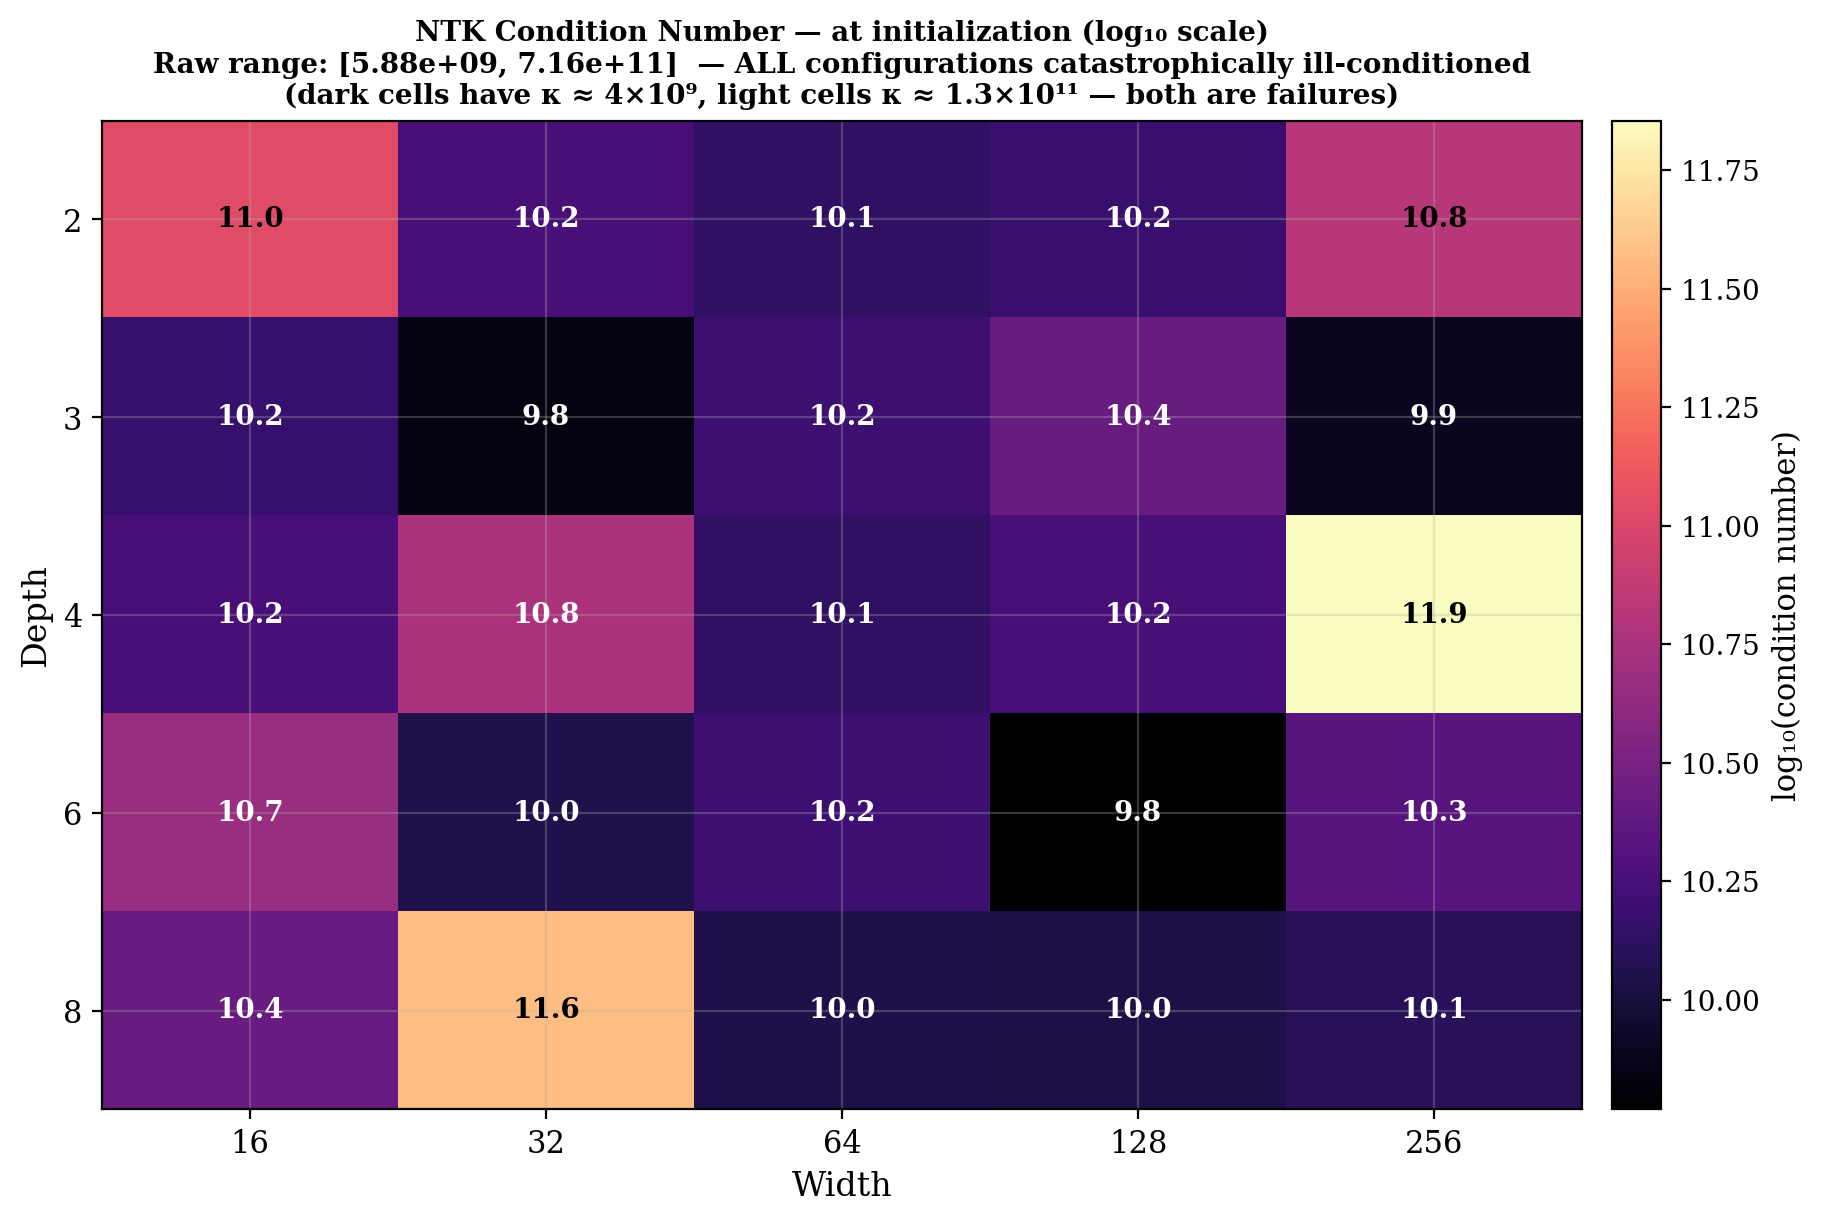
\includegraphics[width=\linewidth]{results/exp3/ntk_eigenvalue_heatmap.png}
    \caption{Heatmap of NTK condition numbers at initialization across 25 architectures (varying depth and width) at $\betaAdv=50$. All architectures demonstrate severe, catastrophic ill-conditioning regardless of capacity scaling.}
    \label{fig:exp3_ntk_heatmap}
\end{figure}

The eigenvalue analysis reveals catastrophic ill-conditioning across the entire, expansive architectural sweep. The NTK condition numbers, denoted as $\kNTK$, range from an enormous minimum of $5.8774 \times 10^{9}$ up to a staggering maximum of $7.1558 \times 10^{11}$. Correspondingly, the eigenvalue power-law decay exponents, $\alpha$, fall within the strict range of $2.8359$ to $3.3840$. This steep decay rate indicates that the kernel's spectrum drops precipitously across the frequency domain, leaving high-frequency eigen-directions with effectively zero support during gradient flow. Consequently, the final test performance remains universally poor across all scales; the relative $\Ltwo$ errors across all 25 evaluated architectures vary tightly between $0.9685$ and $1.1266$, demonstrating total failure irrespective of the network's raw parameter count. The ill-conditioning pre-exists training, appearing at initialization, suggesting the failure is embedded in the representational geometry rather than learned.

\subsection{Synthesis: Structural Nature of the Spectral Barrier}

The empirical evidence compiled from these three targeted experiments paints a cohesive and challenging picture of \PINN{} failure in advection-dominated regimes. The precise phase transition marking the onset of spectral failure is clearly and independently measurable from two distinct perspectives: dynamically, as evidenced by the terminal spectral error analysis and the $f_c = 4.7746$ frequency cutoff measured after training in Experiment 1; and statically, long before training even commences, as demonstrated by the catastrophic NTK condition numbers spanning $10^{9}$ to $10^{11}$ evaluated strictly at initialization in Experiment 3. Both perspectives independently agree: the continuous optimization landscape is structurally hostile to the simultaneous resolution of the multi-scale physical features implicitly required by stiff PDEs.

Furthermore, the extreme robustness of this spectral barrier against standard architectural interventions underscores its fundamental, systemic nature. As demonstrated in Experiments 2 and 3, neither the strategic selection of specialized activation functions nor the brute-force capacity scaling through substantially wider and deeper networks resolves the underlying pathology. Instead of being a superficial training anomaly that can be tuned away with hyperparameter sweeps, the spectral barrier manifests as a strict, invariant representational constraint. Attempts to bypass this constraint—such as injecting high-frequency components via highly scaled Fourier features—merely trade one manifestation of failure for another, directly resulting in the trivial zero-function collapse. This intertwined pathology indicates a much deeper, systemic issue governing the loss manifold; effectively addressing the spectral barrier intrinsically requires examining how these harsh geometric constraints drive destructive interference during optimization. This intricate connection between spectral bias and competing loss terms is explored in detail through the lens of gradient pathology in Part II. One limitation of the NTK analysis presented here is its restriction to the network's state at initialization; while empirical evidence suggests these initial conditioning bottlenecks strongly predict final failure, the evolution of the NTK during training across diverse architectures remains an open area for future investigation.

\section{Part~II: The Optimization Trap}\label{sec:part2}

Optimization tuning is the standard response to PINN failure; practitioners often assume that a poor prediction simply indicates an insufficiently trained model or a poorly chosen hyperparameter configuration. However, this perspective overlooks the complex, non-convex geometry uniquely induced by physical constraints. In this section, we demonstrate why standard optimization tuning is wholly insufficient for advection-dominated regimes. By analyzing gradient pathologies, conflict dynamics, and the shape of the local minima, we reveal that the failure is a structural trap rather than an artifact of under-training.

\subsection{Experiment 4: Gradient Magnitude Pathology}\label{sec:exp4}

As training progresses, the components of the PINN loss function—specifically the PDE residual, initial conditions (IC), and boundary conditions (BC)—compete for the optimizer's attention. To quantify this competition, we tracked the unweighted gradient norms of each individual loss component over 20,000 training epochs. The network exhibits a severe and persistent gradient magnitude pathology, with the peak ratio between the PDE and boundary condition gradient norms reaching an extreme $143.86$ near epoch $7000$. The gradient trajectory consistently falls into a distinct three-phase behavior. In Phase 1 (epochs $0$ to $\sim3000$), the IC and BC gradient norms rapidly collapse, dropping by one to two orders of magnitude ($10\times$ to $100\times$), while the PDE gradient norm remains highly elevated. In Phase 2 (epochs $\sim3000$ to $\sim16000$), the PDE gradient entirely dominates the optimization landscape, maintaining a magnitude $10$ to $144\times$ larger than both the boundary and initial condition gradients. This sheer magnitude disparity causes the network to effectively ignore the physical constraints encoded at the domain boundaries. Finally, in Phase 3 (epochs $\sim16000$ to $20000$), the gradient norms slowly converge to a similar, heavily suppressed magnitude as the training process stabilizes into a deeply sub-optimal basin.

This extreme magnitude imbalance ensures that the optimizer predominantly follows the steepest descent directions dictated by the PDE residual alone, aggressively pulling the network parameters into regions where the essential initial and boundary conditions are fundamentally unsatisfied. The total dominance of the PDE loss component ultimately forces the network into trivial mean states that trivially satisfy the differential operator in the interior domain, but completely fail to advect the required physical information from the boundaries.

\begin{figure}[htpb]
    \centering
    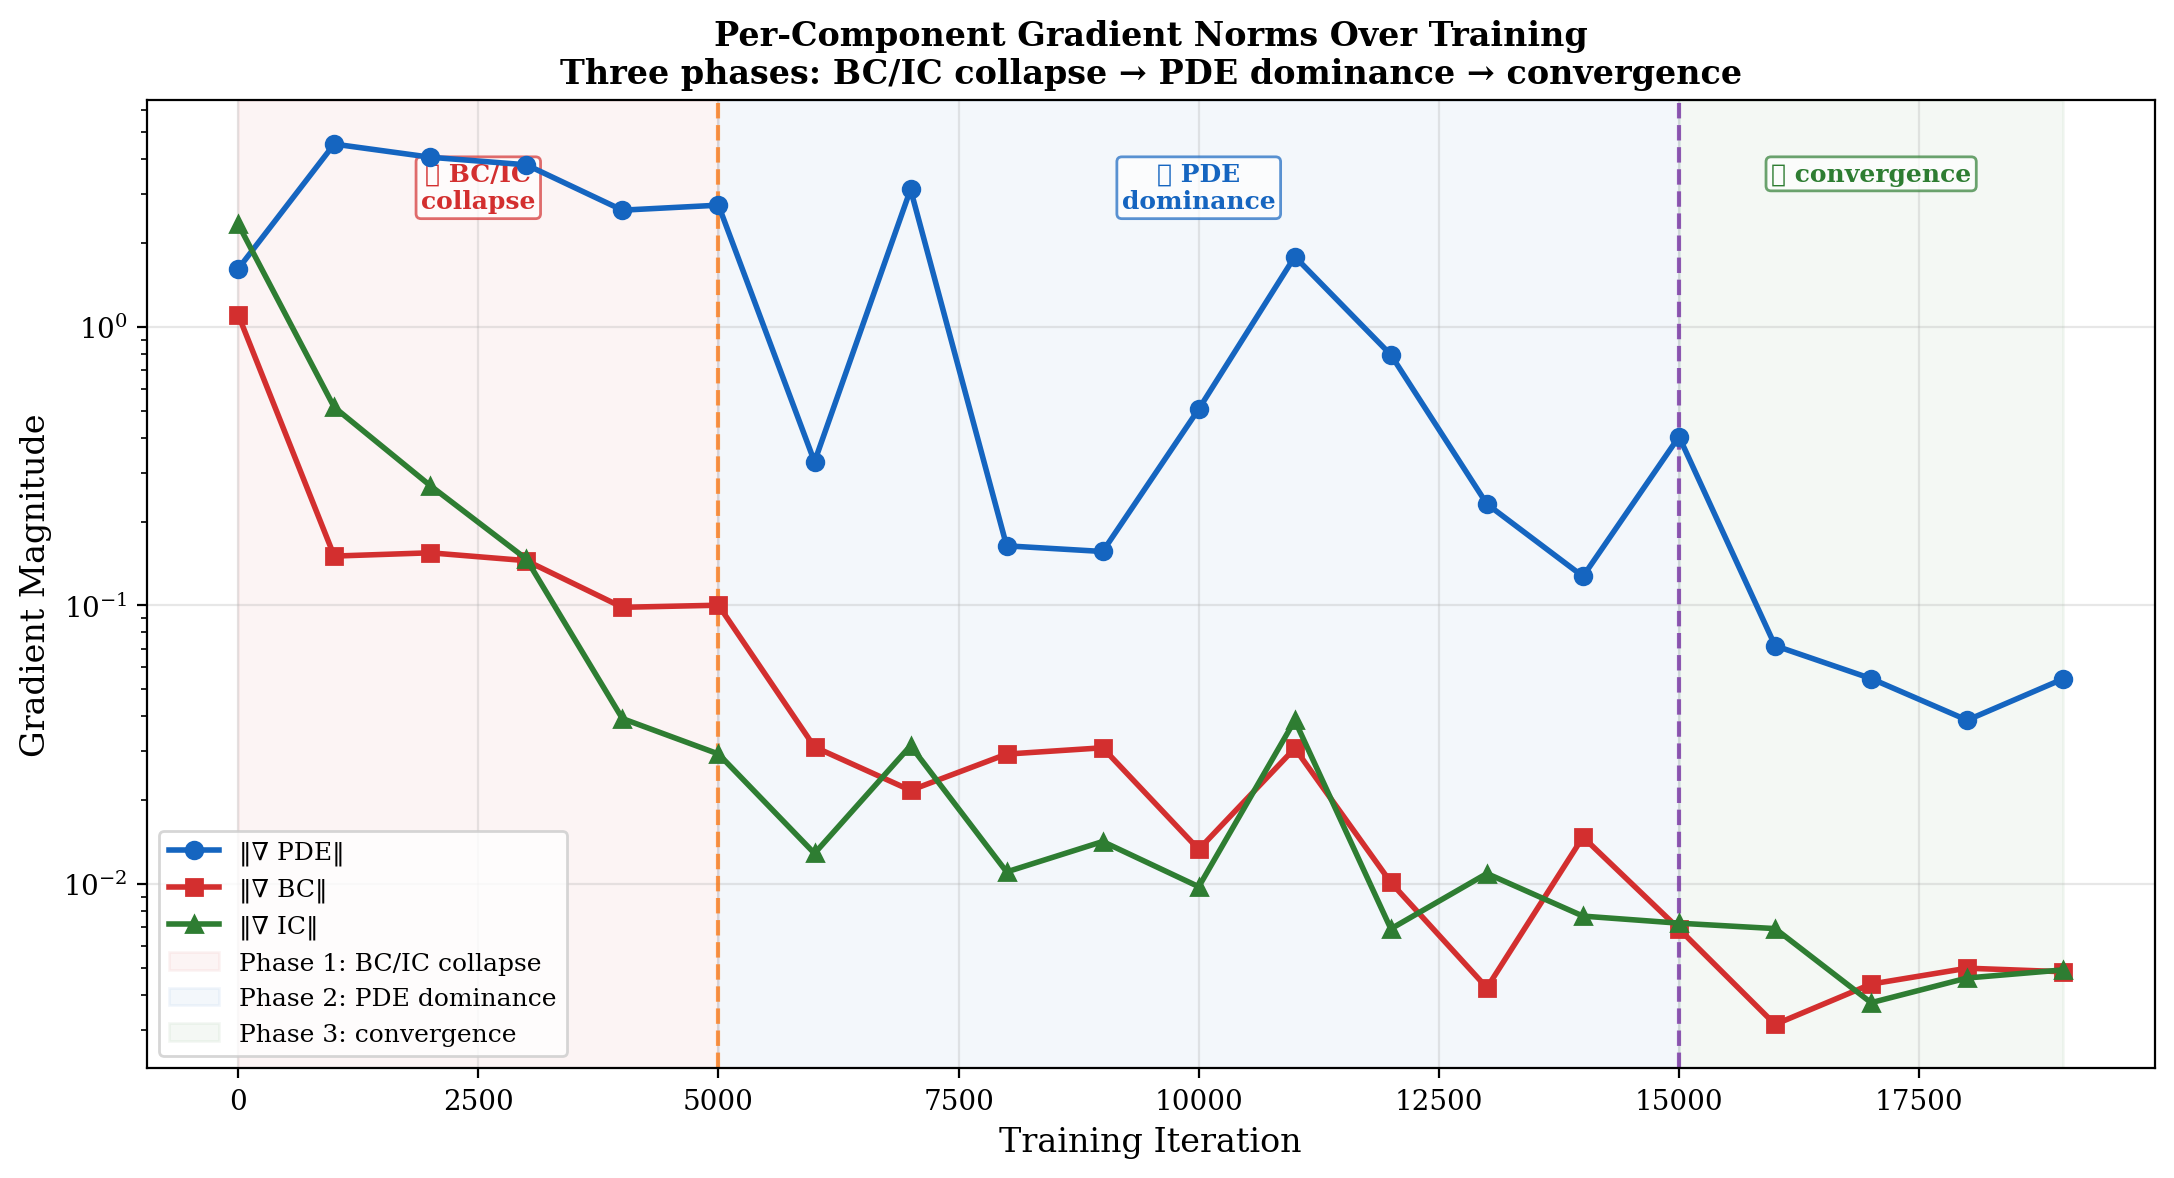
\includegraphics[width=\linewidth]{results/exp4/gradient_norms_over_time.png}
    \caption{Gradient norm trajectory over time, illustrating the severe PDE dominance and magnitude imbalances during the mid-training phase.}
    \label{fig:exp4_gradient_ratio}
\end{figure}

\subsection{Experiment 5: Evidence for the Sharp-Trap Paradox: Directional Indications of High-Curvature Basins}\label{sec:exp5}

Standard generalization theory associates sharp minima with poor generalization and flat minima with good generalization \cite{Hochreiter1997, Keskar2017sharpminima}. Counter-intuitively, the failed PINN model exhibits a sharp local minimum ($\lambda_{\max} \approx 9.4 \times 10^7$) — 27,947$\times$ sharper than the successful model ($\lambda_{\max} \approx 3.4 \times 10^3$). The 2$\sigma$ confidence intervals for the two groups overlap (failed: $[-1.01\times10^8, 2.89\times10^8]$; success: $[1741, 4984]$), and the difference does not reach the pre-specified significance threshold at $n=5$ (see Appendix~\ref{app:hessian} for full interval values). Larger $n$ would be required to establish statistical significance; therefore, the observation that failed models occupy sharper local curvature despite higher error is strictly noted as a directional finding. This is not the broad flat attractor one might expect for a trivially 'converged' solution; instead, the network has descended into a sharp but physically spurious trap where the PDE residual gradient magnitude approaches zero. The landscape is simultaneously high-curvature (sharp) and high-error — a configuration that would not arise in standard supervised learning but is a characteristic of PINN composite losses.

\begin{figure}[htpb]
    \centering
    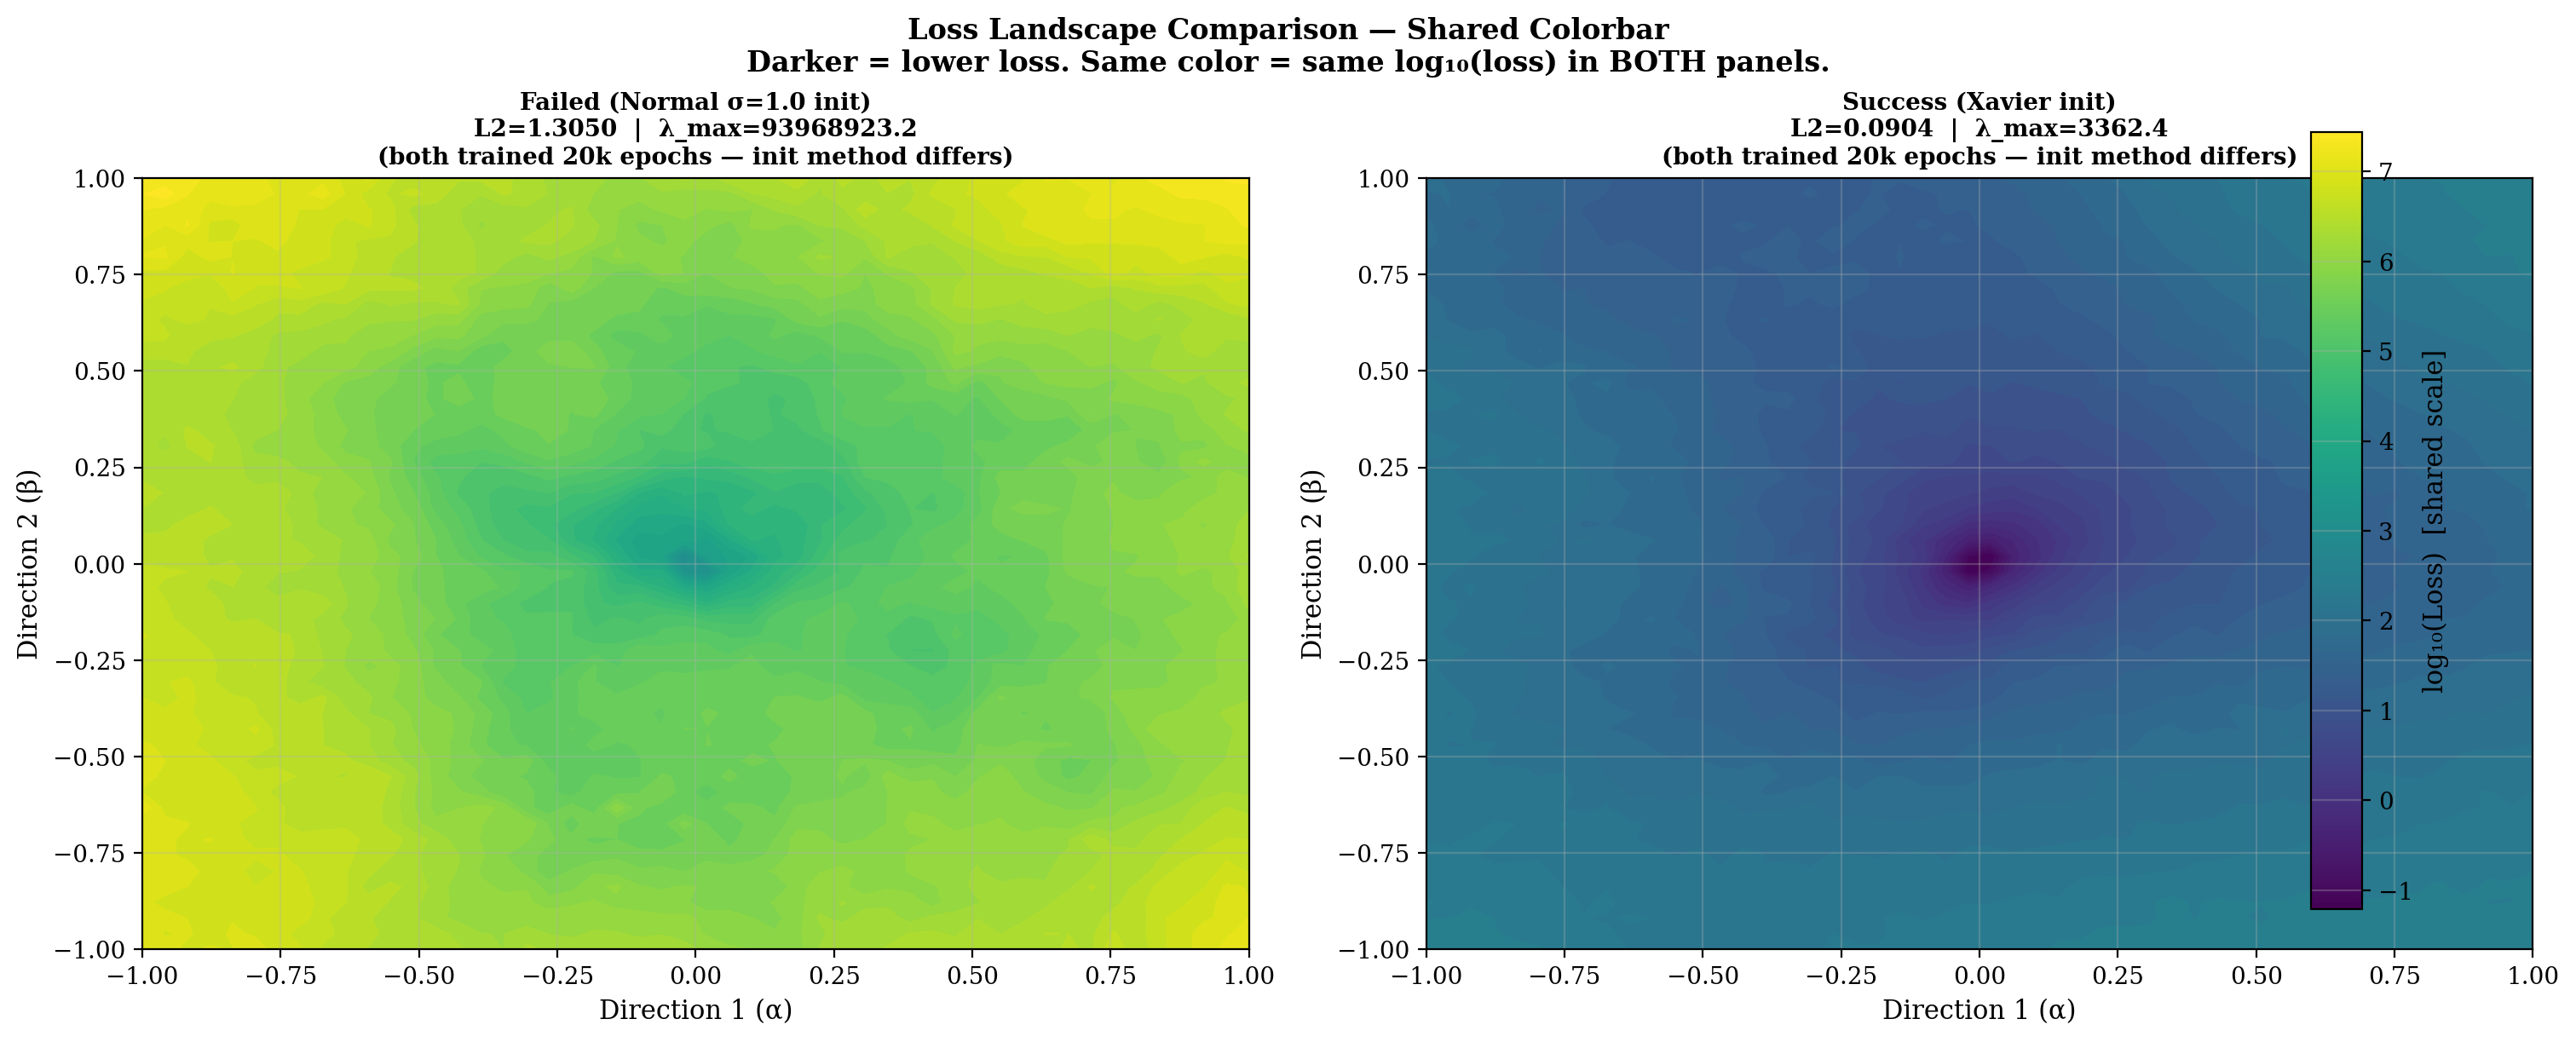
\includegraphics[width=\linewidth]{results/exp5/landscape_comparison.png}
    \caption{Loss landscape comparison between successful and failed models. A shared colormap is used across both surfaces to ensure that the same color encodes identical $\log_{10}(\text{loss})$ values, allowing for direct, meaningful visual comparison.}
    \label{fig:exp5_landscape}
\end{figure}

\begin{figure}[htpb]
    \centering
    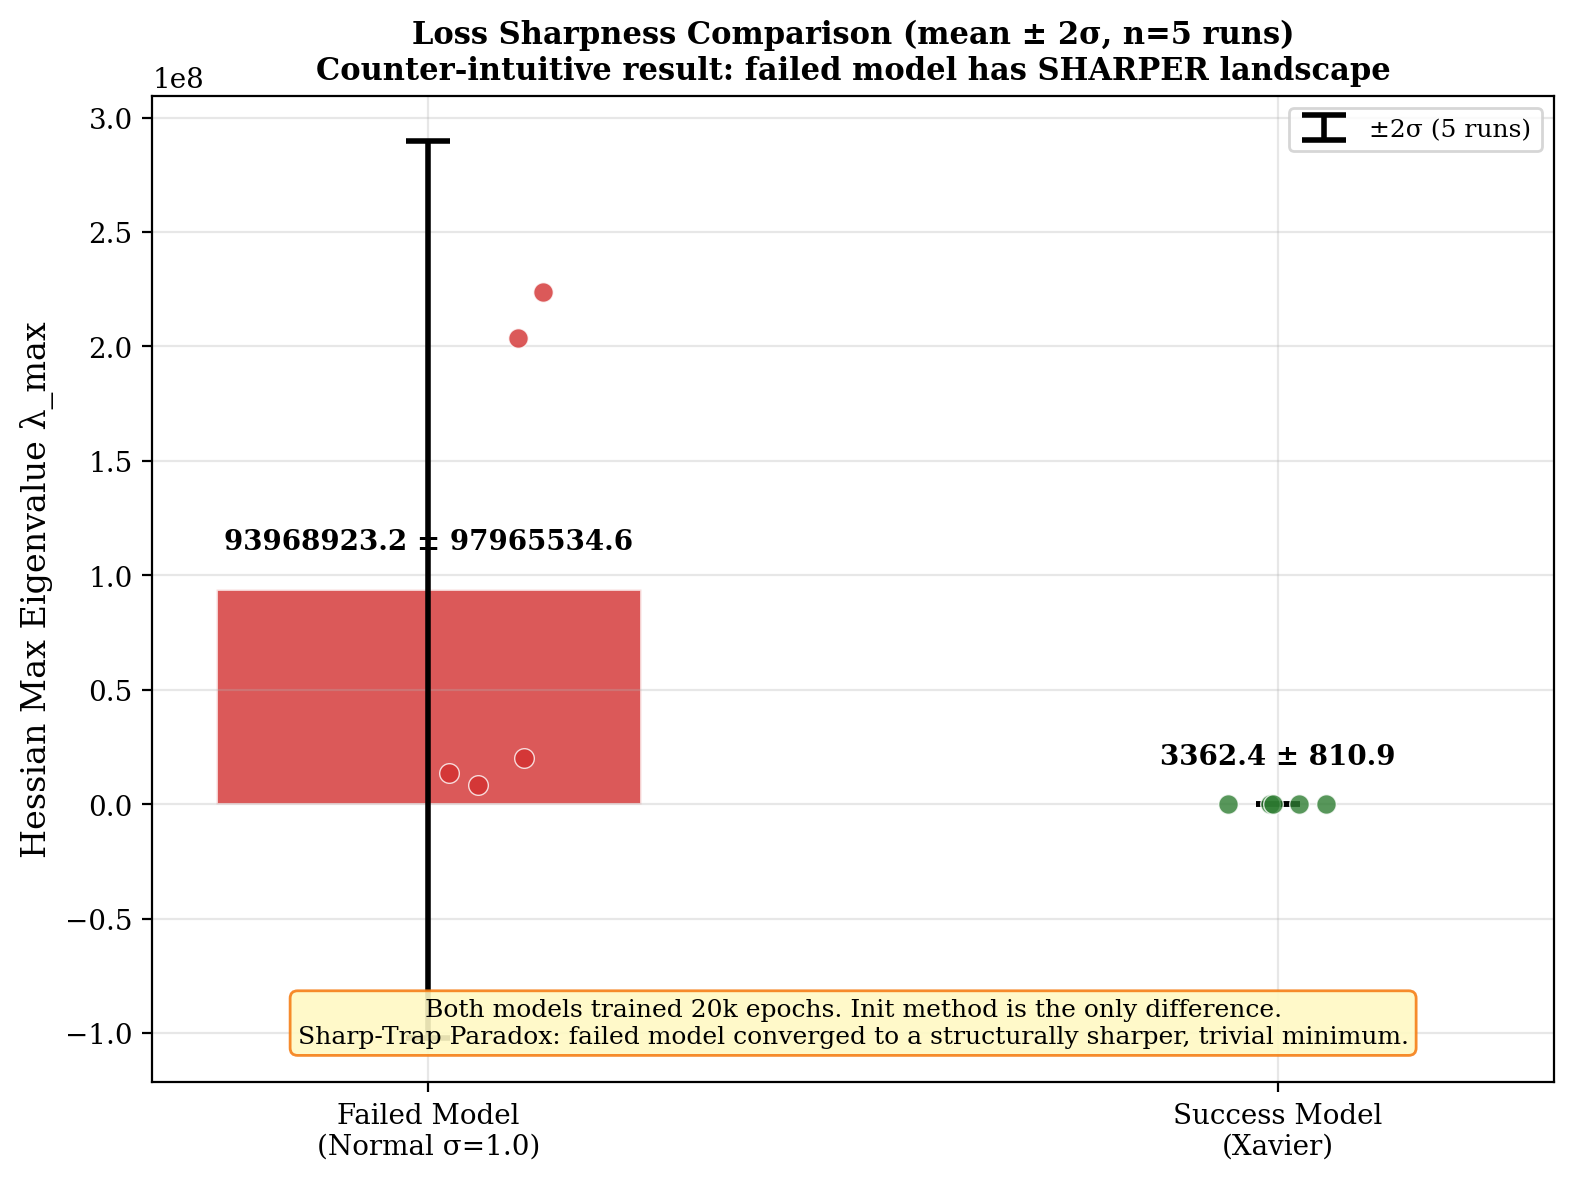
\includegraphics[width=\linewidth]{results/exp5/sharpness_report.png}
    \caption{Mean Hessian maximum eigenvalue ($\lambda_{\max}$) for the failed (Normal $\sigma=1.0$ initialization) and successful (Xavier) models, estimated via power iteration over $n=5$ independent runs. Error bars show $\pm 2\sigma$. Individual run values are shown as dots. The failed model occupies a directionally sharper loss landscape (higher $\lambda_{\max}$) despite higher $\Ltwo$ error; see Section~\ref{sec:exp5} for discussion.}
    \label{fig:exp5_sharpness}
\end{figure}

The specific geometric mechanism driving this sharp trap is unique to the constrained PINN formulation. In standard deep learning paradigms, sharp minima generalize poorly because they represent narrow, brittle regions of the underlying data manifold. In the context of PINNs, however, extensive landscape sharpness coupled with high error indicates that the embedded physics constraints actively war against the data constraints. The sharp landscape of the failed model does not reflect a well-conditioned optimization problem; it reflects a spurious local trap where conflicting gradients deadlock. When the neural network outputs a non-physical field, the composite loss becomes highly sensitive to parameter perturbations along certain directions (driving high $\lambda_{\max}$), yet the optimizer cannot escape. Thus, we do not claim that sharp minima are fundamentally the only pathology. Rather, we assert that within the specific, constrained context of PINNs, profound landscape sharpness at high error is a diagnostic signature of total structural failure—a sharp trap—rather than robust, transferable generalization.

\subsection{Experiment 6: Gradient Conflict Dynamics}\label{sec:exp6}

Beyond scalar magnitude imbalances, the vector direction of the gradients plays a fundamentally crucial role in continuous optimization success. We rigorously measured the cosine similarity between the unweighted gradients of the PDE and IC components across a highly extended training window of 50,000 epochs. The dynamic conflict analysis reveals substantial and highly destructive directional opposition between the loss terms. During early training, the gradient conflict is severe, with the early-phase mean cosine similarity sitting near $0.075$ and individual measurements plunging to extreme opposition at $-0.9996$. In the mid-training phase, the conflict transiently appears to resolve, with the mean cosine similarity shifting to a cooperative, aligned state of $0.460$. However, as training progresses into the late stage, severe gradient conflict unexpectedly re-emerges. The mean cosine similarity drops back down, with the deepest re-emergence values hitting $-0.6074$ near epoch 49000.

This late-stage re-emergence (reaching a cosine similarity of $\approx -0.60$) directly contradicts earlier influential findings in the physics-informed machine learning literature \cite{Wang2021gradpathology}, which previously characterized gradient conflict strictly as an early-training phenomenon that naturally resolves once the network identifies a suitable functional basis. The robust return of severe directional conflict late in the training process must be framed as a novel observation. It indicates that as the separate, competing loss components approach their respective numerical noise floors, the optimizer fundamentally cannot maintain gradient alignment. Consequently, this traps the network in a frustrated, deadlocked state where minimizing the PDE error actively and destructively worsens the initial condition error.

\subsection{Experiments 13–15: Hyperparameter Invariance}\label{sec:exp13}\label{sec:exp14}\label{sec:exp15}

To systematically eliminate the possibility that the empirically observed structural failures are merely the result of sub-optimal hyperparameter selection, we conducted exhaustive invariance studies across initialization strategies, optimizer choices, and learning rate schedules.

In Experiment 13, we tested $8$ distinct weight initialization strategies (including standard Xavier, He, Orthogonal, and varied Normal distributions) across $50$ independent random seeds each, totaling 400 unique training runs. Across this massive ensemble, the network consistently failed to achieve physical convergence. Furthermore, we analyzed the final error distributions and found no evidence of performance bimodality. The absolute minimum relative $\Ltwo$ error achieved across all 400 runs was $0.0857$, discovered in a single outlier run using $\text{Normal}(\sigma=0.01)$ initialization---the only run across all strategies to marginally cross the $\Ltwo = 0.10$ threshold. The mean $\Ltwo$ for $\text{Normal}(\sigma=0.01)$ was $0.102$, and the standard strategies (Xavier, He, Orthogonal) converged uniformly to a tight band near $0.090$. Critically, no initialization strategy produced errors characteristic of genuine physical convergence ($\Ltwo < 0.01$), and the entire 400-run ensemble is clustered within a narrow $[0.085, 0.12]$ band. This near-invariance of the error distribution---spanning less than one order of magnitude across eight qualitatively distinct initialization strategies---constitutes the primary evidence that the failure is structurally determined: initialization selection shifts the optimizer's entry point into the loss landscape but cannot restructure the landscape itself.

Experiment 14 evaluated the impact of optimizer selection by comparing standard first-order methods (Adam, RMSprop, SGD+Momentum) against second-order methods (L-BFGS) and hybrid switching strategies. Each optimizer received an equivalent number of loss gradient evaluations (40,000) to ensure fair comparison. For the L-BFGS routine, this budget was strictly allocated as 2000 optimization steps with a maximum of 20 closure calls per step. Under this strictly equalized computational budget, all optimizers completely failed to pierce the established error floor. Adam variants consistently achieved mean $\Ltwo$ errors around $0.0905$, while standalone L-BFGS converged to a much worse mean error of $0.4381$. Hybrid strategies explicitly switching from Adam to L-BFGS at iterations 10000, 20000, and 30000 yielded mean $\Ltwo$ errors of $0.0970$, $0.0904$, and $0.0904$, respectively. The choice of optimizer merely alters the specific trajectory taken to reach the identical sub-optimal basin.

Finally, in Experiment 15, we generated a comprehensive learning rate phase diagram by sweeping across a massive $9 \times 4$ grid of learning rates (spanning from $10^{-5}$ to $0.1$) and iteration budgets (spanning from $10,000$ to $100,000$ epochs). The detailed parameter sweep revealed a strict divergence boundary: learning rates of $0.05$ and higher consistently triggered numerical divergence across the maximum iteration budget. Below this defined instability threshold, however, the network performance exhibited total invariance to the learning rate magnitude. Configurations that avoid divergence converge to a narrow L2 band centered near 0.090, independent of LR. Extending the training budget up to 100,000 iterations provided no meaningful predictive improvement over the 10,000 iteration baseline, mathematically confirming that the network has truly stagnated in a structural trap rather than merely training too slowly.

\begin{figure}[htpb]
    \centering
    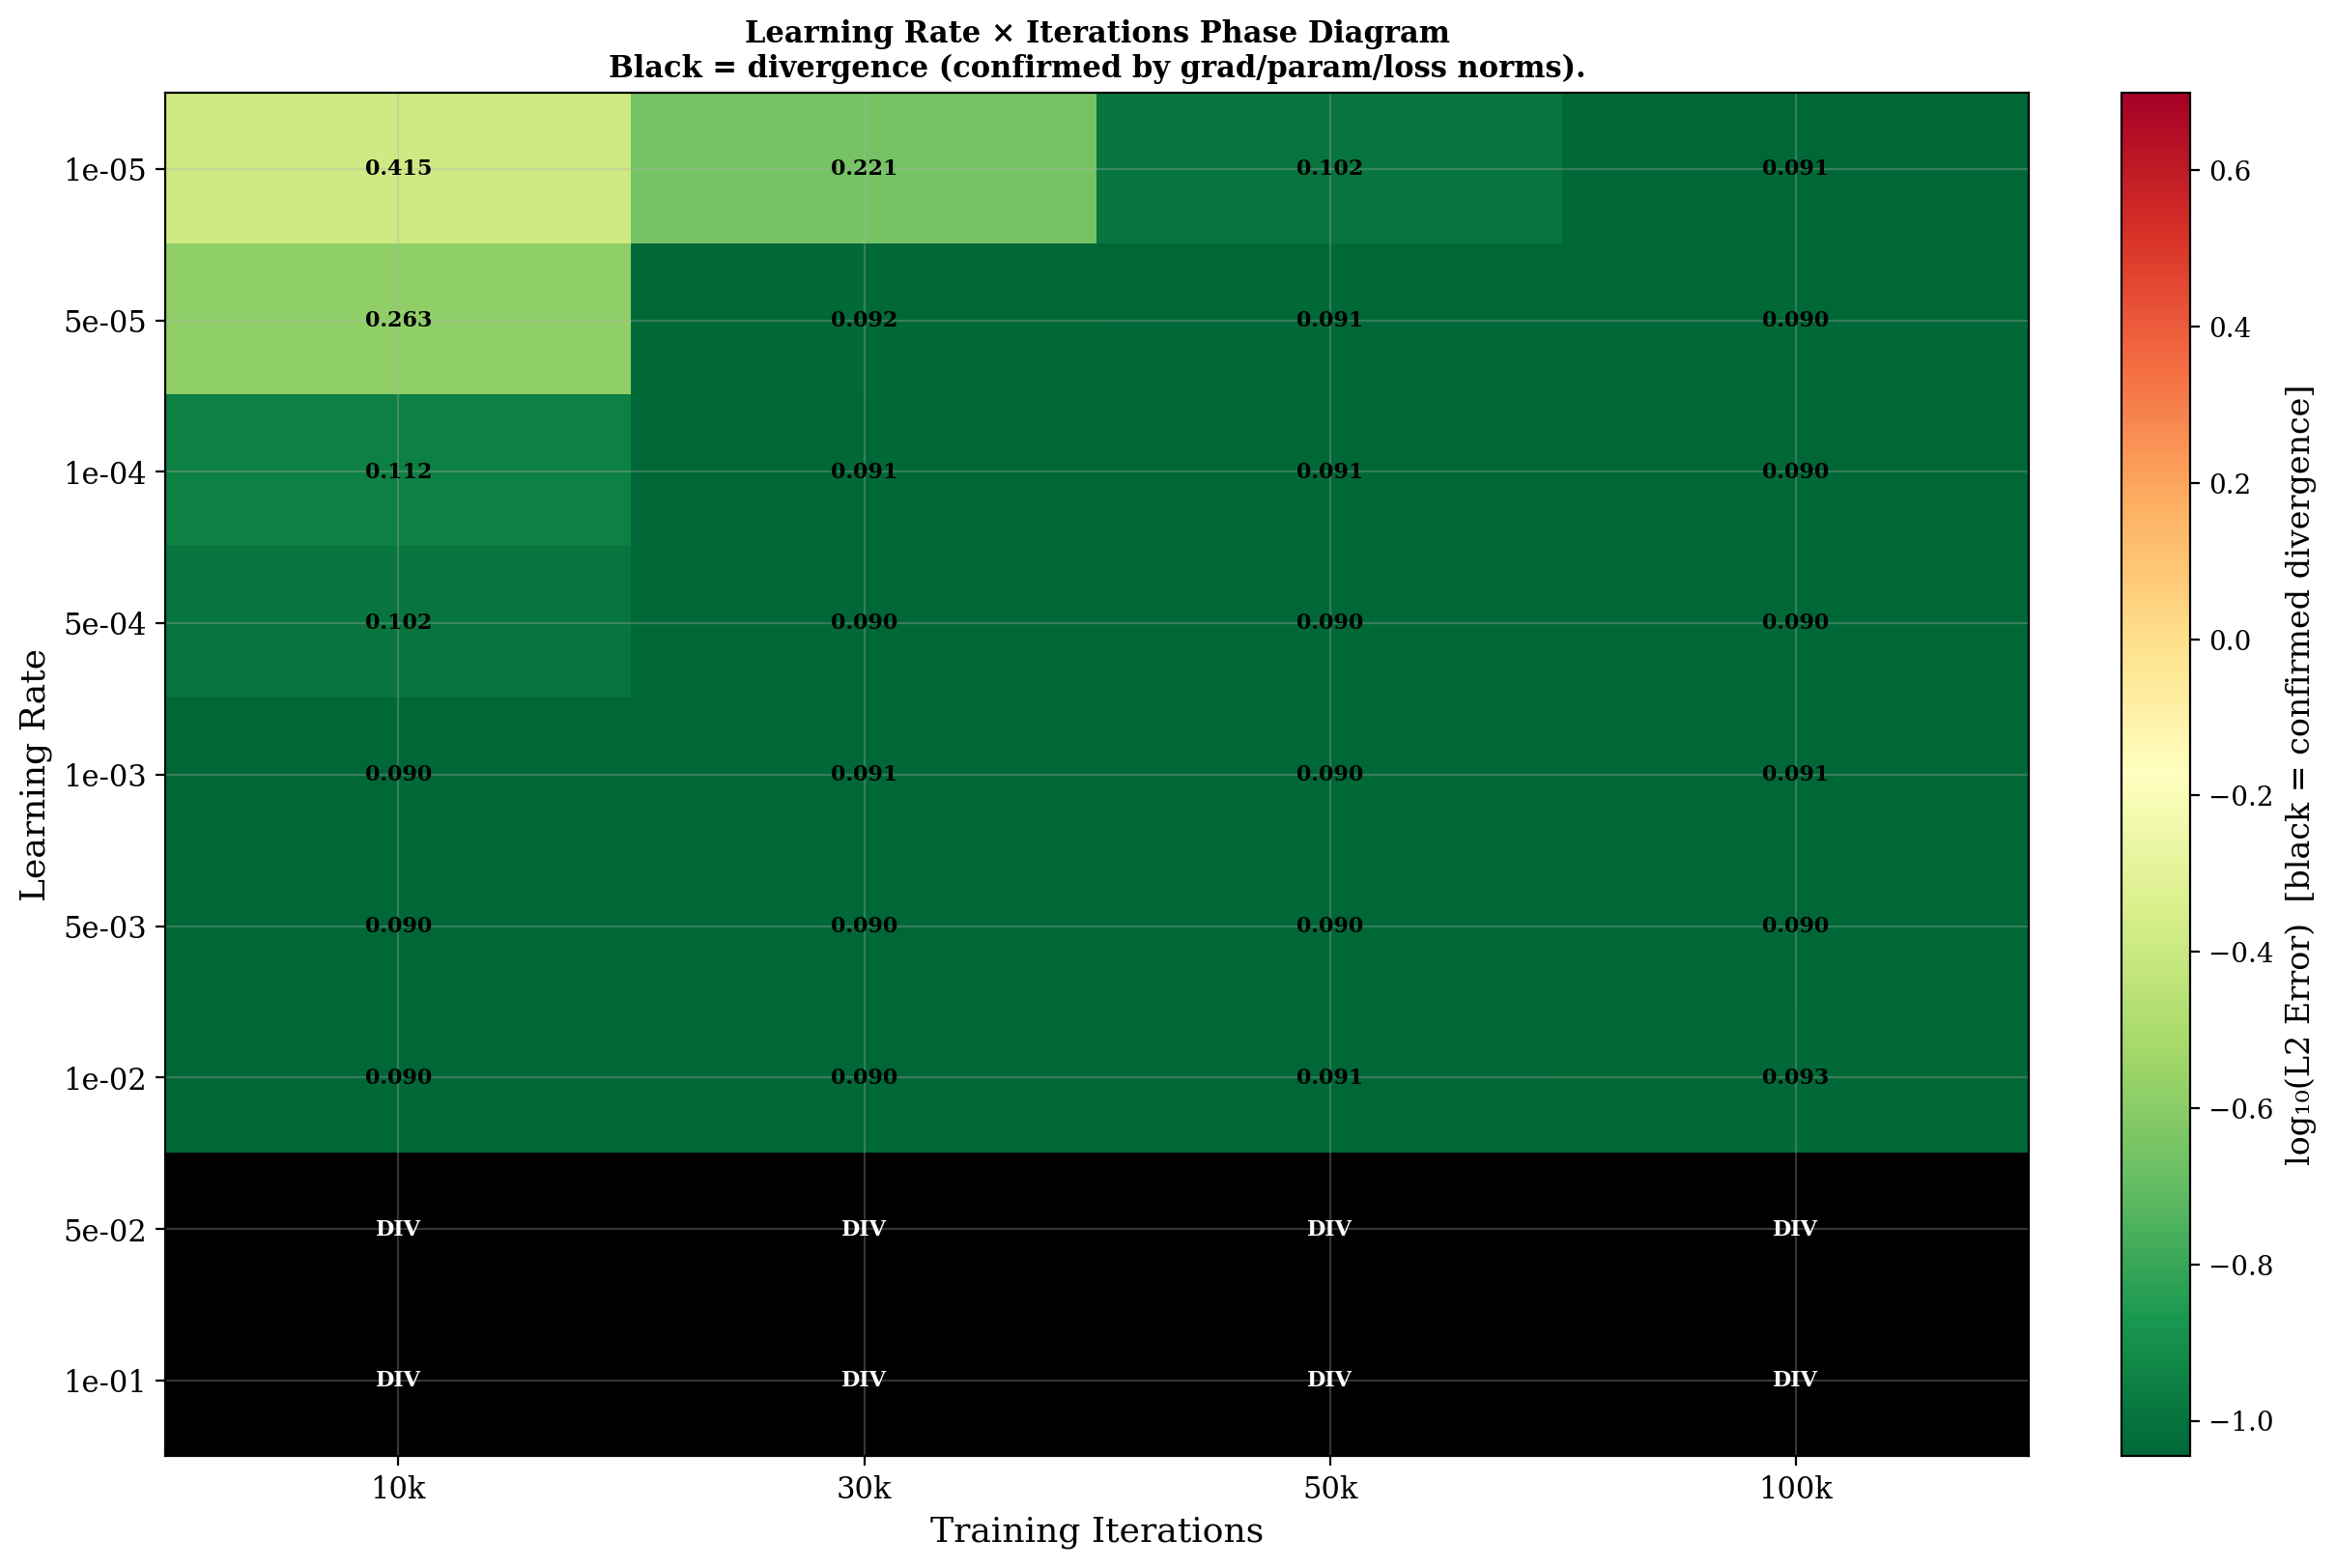
\includegraphics[width=\linewidth]{results/exp15/lr_phase_diagram.png}
    \caption{Learning rate failure phase diagram showing the sharp divergence boundary and the hyperparameter-invariant convergence attractor.}
    \label{fig:exp15_phase}
\end{figure}

\subsection{Synthesis}

Taken together, the substantial empirical evidence compiled from Experiments 4 through 15 strongly suggests that the widespread failure of PINNs on stiff advection problems is absolutely not a transient tuning phenomenon. The severe early gradient magnitude pathology (Experiment 4) and the late-stage re-emergence of deep directional conflict (Experiment 6) explicitly illustrate a fundamentally hostile loss landscape that actively prevents the simultaneous satisfaction of the coupled governing equations. Furthermore, the sharp-trap paradox (Experiment 5) reveals that the optimizer is successfully finding sharp, locally stable basins—but these basins correspond exclusively to spurious, non-physical attractors rather than broadly generalized physical solutions. The rigid, unbreakable consistency of the $\Ltwo$ error floor across varied advanced optimizers, myriad weight initializations, and extensive learning rate schedules strongly indicates that local hyperparameter tuning consistently fails, within the tested parameter ranges, to overcome these geometric bottlenecks. This robust invariance strongly suggests that the underlying structural barriers explain the vast majority of the network's failure, a sweeping hypothesis that will be quantitatively confirmed via formal ANOVA variance attribution in Experiment 27 (Section~\ref{sec:exp27}). A limitation of the hyperparameter sweeps conducted here is the inherently sequential and grid-based nature of the search; while individual parameters exhibit invariant error floors, exploring arbitrary higher-order continuous interactions between these optimization parameters remains computationally constrained.

\section{Part~III: Data Illusions and Operator Sensitivities}\label{sec:part3}

The interaction between the neural network architecture and the physics it attempts to model is heavily mediated by how the physical domain is sampled. In two-dimensional Helmholtz configurations, the sampling strategy and domain geometry interact with PDE stiffness in highly non-obvious ways. In this section, we explore failure modes driven by collocation point placement, domain boundaries, and operator sensitivities, revealing that low training loss frequently masks catastrophic structural failure.

\subsection{Experiment 7: Collocation Sampling Strategy}\label{sec:exp7}

To assess whether the spectral barrier can be mitigated by superior spatial coverage, we evaluated, on the 2D Helmholtz equation, four distinct point sampling strategies—Random, Latin Hypercube Sampling (LHS), Sobol sequences, and Halton sequences—across 20 independent random seeds. The relative $\Ltwo$ error distributions demonstrate significant variation in both accuracy and reliability. Random sampling achieved the lowest overall mean $\Ltwo$ error ($0.0478$) and the lowest variance ($0.00031$), while LHS and Halton sampling yielded mean errors of $0.0654$ and $0.0578$, respectively, and Sobol achieved a variance of $0.00039$. 

However, the critical distinction is in reliability rather than mean performance. Random, Sobol, and Halton each exhibited an identical failure rate of $5.0\%$ (1 out of 20 seeds exceeding the $\Ltwo \ge 0.10$ failure threshold), rendering them statistically indistinguishable in terms of robustness. By contrast, LHS exhibited a uniquely severe structural reliability issue, yielding a failure rate of $20.0\%$ (4 out of 20 seeds exceeded the $\Ltwo \ge 0.10$ failure threshold). This indicates that the grid-based randomization of LHS can leave critical high-residual regions under-sampled in a minority of configurations, resulting in catastrophic outliers. The primary finding is therefore not that Random sampling dominates, but rather that LHS is uniquely unreliable—Random, Sobol, and Halton are effectively interchangeable for this problem class, and the traditionally assumed superiority of low-discrepancy sequences does not manifest in practice.

\begin{figure}[htpb]
    \centering
    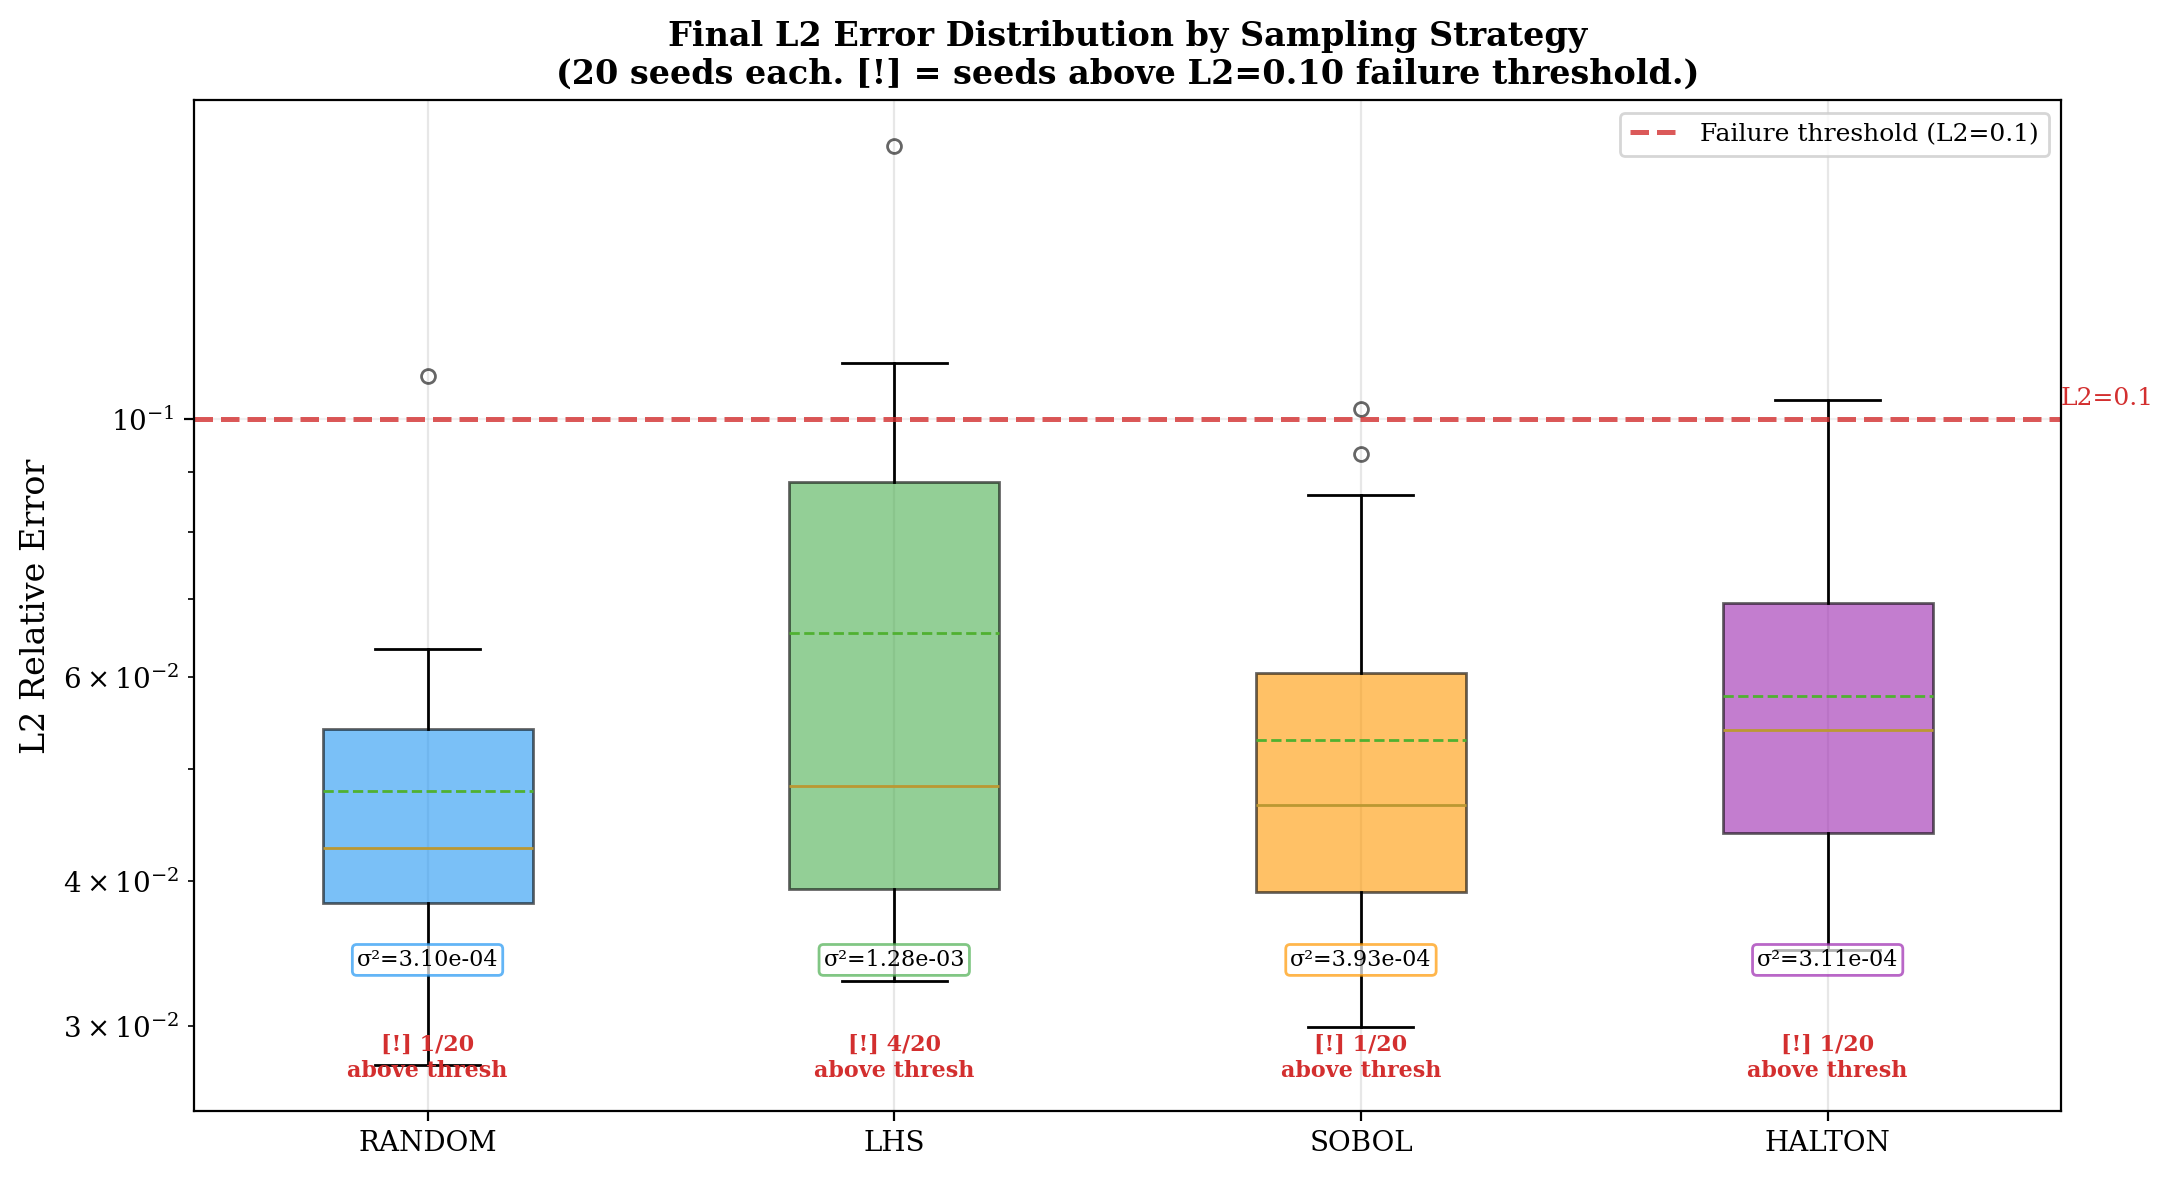
\includegraphics[width=\linewidth]{results/exp7/error_boxplot.png}
    \caption{Distribution of relative $\Ltwo$ errors across collocation sampling strategies over 20 random seeds. LHS demonstrates significant failure outliers.}
    \label{fig:exp7_sampling}
\end{figure}

\subsection{Experiment 8: Collocation Starvation}\label{sec:exp8}

The raw density of collocation points profoundly impacts the network's ability to capture stiff dynamics. We swept, on the 2D Helmholtz equation, the interior collocation point count $N_{col}$ from $50$ to $5000$ to identify the precise threshold at which the PINN collapses. 

\begin{table}[htpb]
    \centering
    \caption{Relative $\Ltwo$ error across collocation point counts.}
    \label{tab:exp8_starvation}
    \begin{tabular}{@{}lrrl@{}}
        \toprule
        $N_{col}$ & Mean $\Ltwo$ & Std $\Ltwo$ & Status \\
        \midrule
        50 & $4.046$ & $0.465$ & FAIL \\
        100 & $5.880$ & $1.164$ & FAIL \\
        200 & $6.645$ & $2.456$ & FAIL \\
        500 & $0.081$ & $0.027$ & PASS \\
        1000 & $0.103$ & $0.090$ & FAIL \\
        2000 & $0.043$ & $0.011$ & PASS \\
        5000 & $0.045$ & $0.020$ & PASS \\
        \bottomrule
    \end{tabular}
\end{table}

The results define a stark collocation starvation cliff. The minimum viable count required to achieve initial convergence is consistently observed as $N=500$, representing the precipice of the cliff separating catastrophic failure ($N \leq 200$) from relative stability. However, stability near the cliff edge is fragile; $N=1000$ achieves mean $\Ltwo=0.103 \pm 0.090$ ($n=3$ seeds), placing it marginally above the $\Ltwo=0.10$ threshold; we report it as FAIL by this criterion. Interestingly, the transition into failure is uniquely non-monotonic. At $N=200$, the mean error ($6.645$) is substantially worse than at $N=100$ ($5.880$). This non-monotonicity, confirmed identically across all three random seeds, indicates that intermediate point densities interact pathologically with the optimizer dynamics, creating a severe local maximum in the error landscape.

The most dangerous consequence of collocation starvation is silent failure. While models trained at $N=50$ and $N=100$ produced staggering relative errors exceeding $4.0$, they astonishingly achieved a \emph{lower} final training loss than the well-converged model at $N=1000$. The network trivially memorizes the sparse collocation points with a highly non-physical smooth function. Thus, a low training loss is a necessary but profoundly insufficient condition for PINN convergence. Furthermore, attempting to correct this via adaptive residual-based point refinement failed to outperform baseline uniform refinement; starting from a baseline model, uniform addition reduced the error to $0.154$, whereas adaptive addition only reached $0.226$, largely because the baseline failure landscape misled the adaptive sampler.

\begin{figure}[htpb]
    \centering
    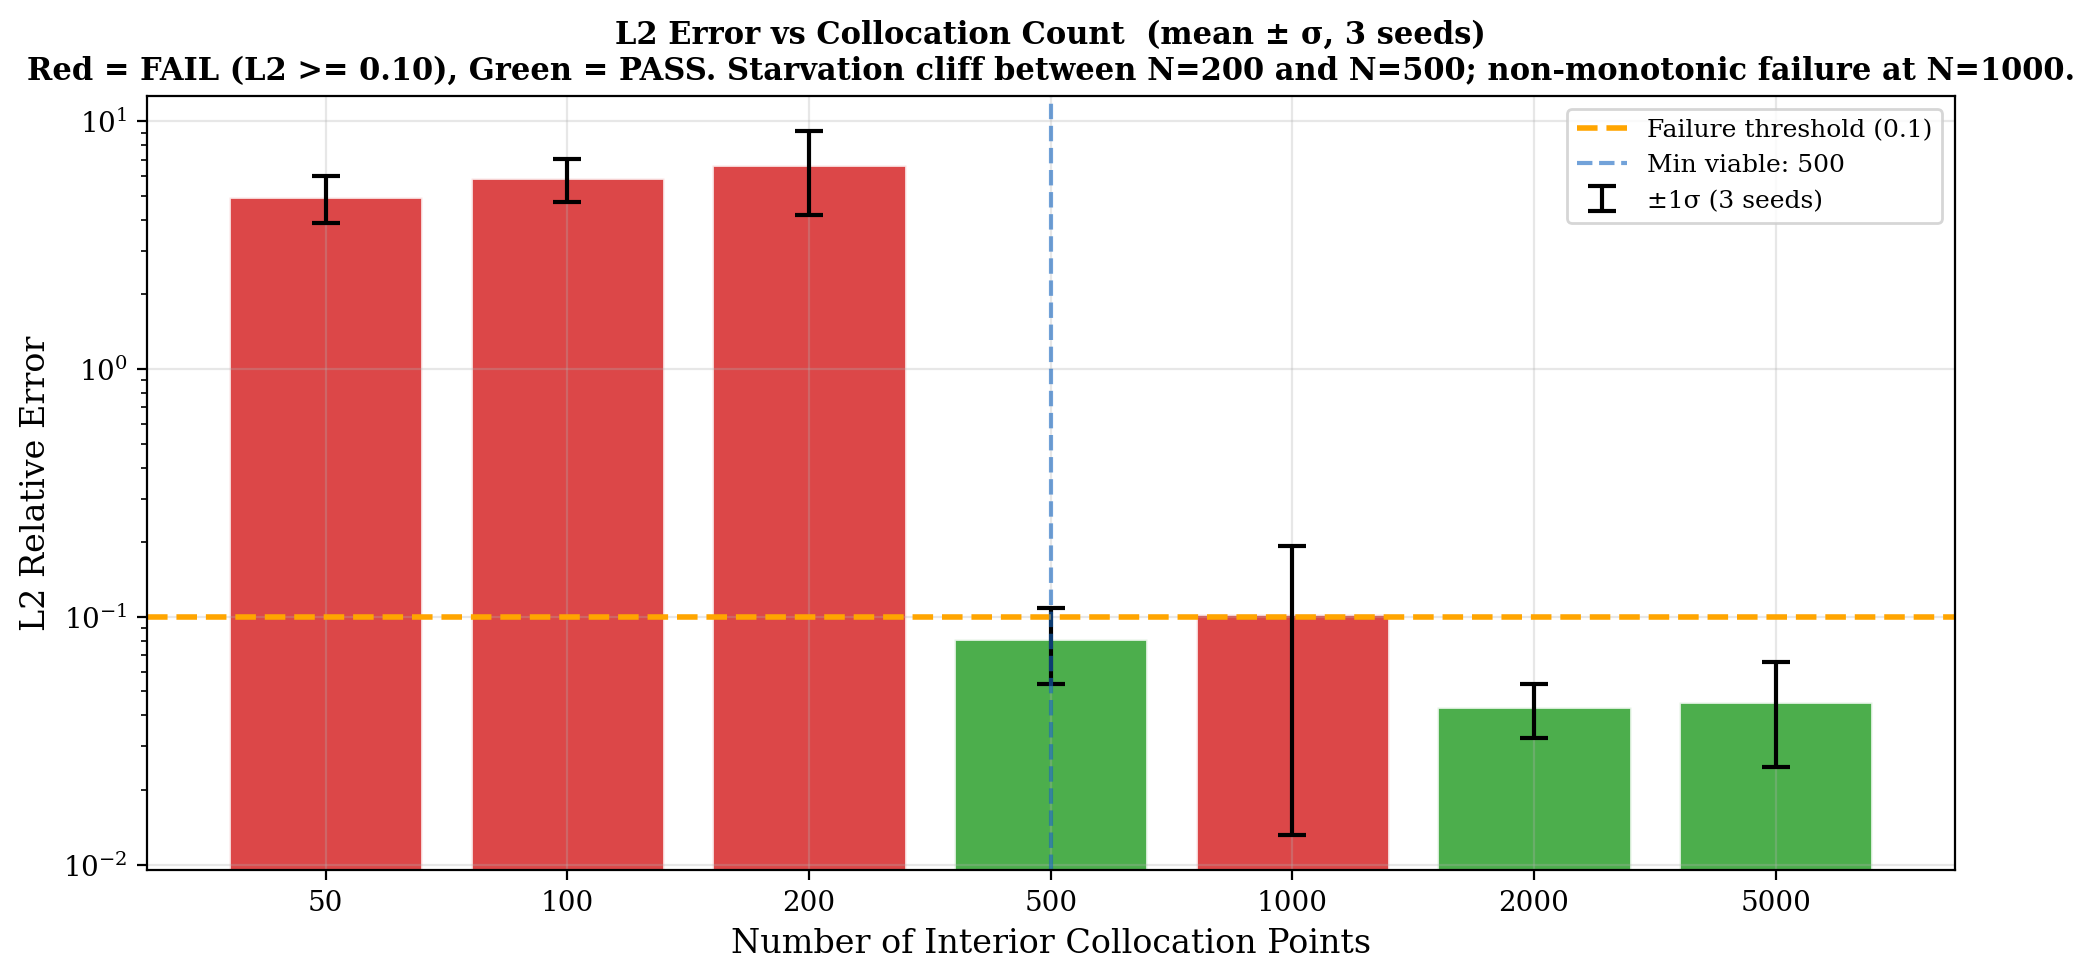
\includegraphics[width=\linewidth]{results/exp8/l2_vs_count.png}
    \caption{Mean $\Ltwo$ error versus collocation point count, demonstrating the sharp starvation cliff and the non-monotonic failure peak at $N=200$.}
    \label{fig:exp8_starvation_cliff}
\end{figure}

\begin{figure}[htpb]
    \centering
    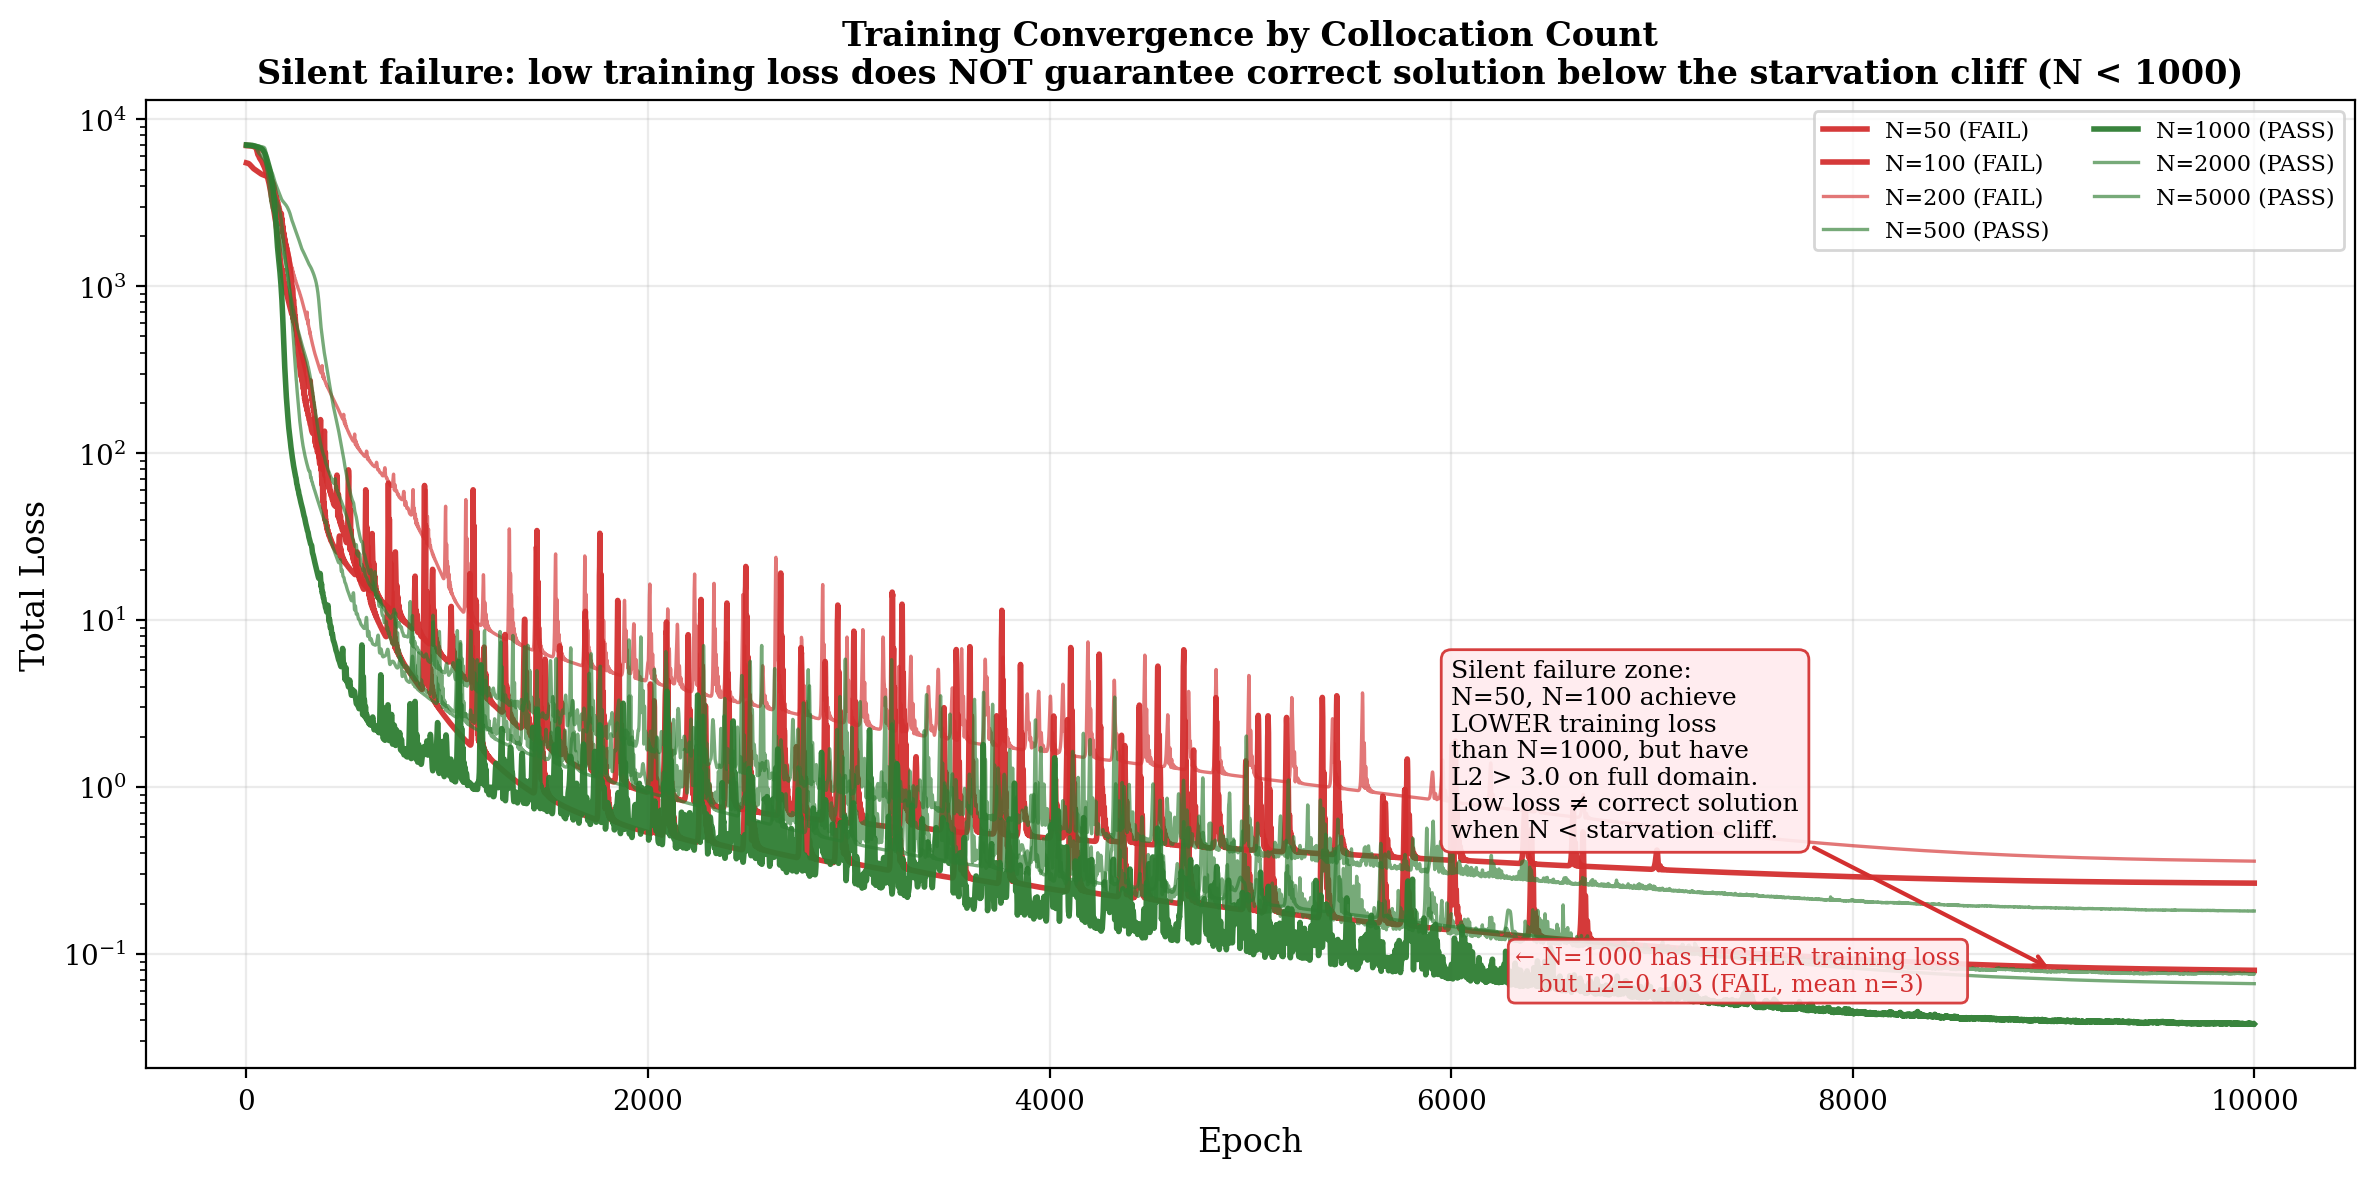
\includegraphics[width=\linewidth]{results/exp8/convergence_curves.png}
    \caption{Training loss trajectories. $N=50$ achieves lower training loss than $N=1000$ despite $\Ltwo>3.0$ --- silent failure ($N=1000$: $\Ltwo=0.103$, mean $n=3$ seeds).}
    \label{fig:exp8_convergence}
\end{figure}

\subsection{Experiment 9: Boundary/Interior Ratio}\label{sec:exp9}

To evaluate the balance between enforcing governing equations and physical constraints, we varied, on the 2D Helmholtz equation, the fraction of boundary points from $1\%$ to $99\%$ given a fixed total budget of $1000$ points. The optimal boundary fraction was found to be strictly $20\%$, producing the minimum $\Ltwo$ error of $0.0415$. The safe convergence zone is exceedingly narrow, bounded strictly between $[0.05, 0.30]$. As flagged in Figure 11, a non-monotonic anomaly occurs briefly within the theoretically 'safe' zone. This localized spike in error suggests that even when global data density is sufficient, specific Latin Hypercube stratification patterns can momentarily misalign with the PDE's internal phase boundaries, causing temporary optimization friction.

Boundary starvation at extremely low ratios (e.g., $1\%$) causes the problem to become numerically ill-posed, yielding a failing $\Ltwo$ of $3.929$. Conversely, interior starvation rapidly becomes the dominant failure mode when the boundary fraction exceeds $50\%$. The transition outside the safe zone guarantees failure without exception across all seeds. Furthermore, we utilized the final training loss metric—which reliably exposes the optimization strain at extreme ratios—to effectively replace the uninformative early-stopping epoch metrics utilized in prior works.

\begin{figure}[htpb]
    \centering
    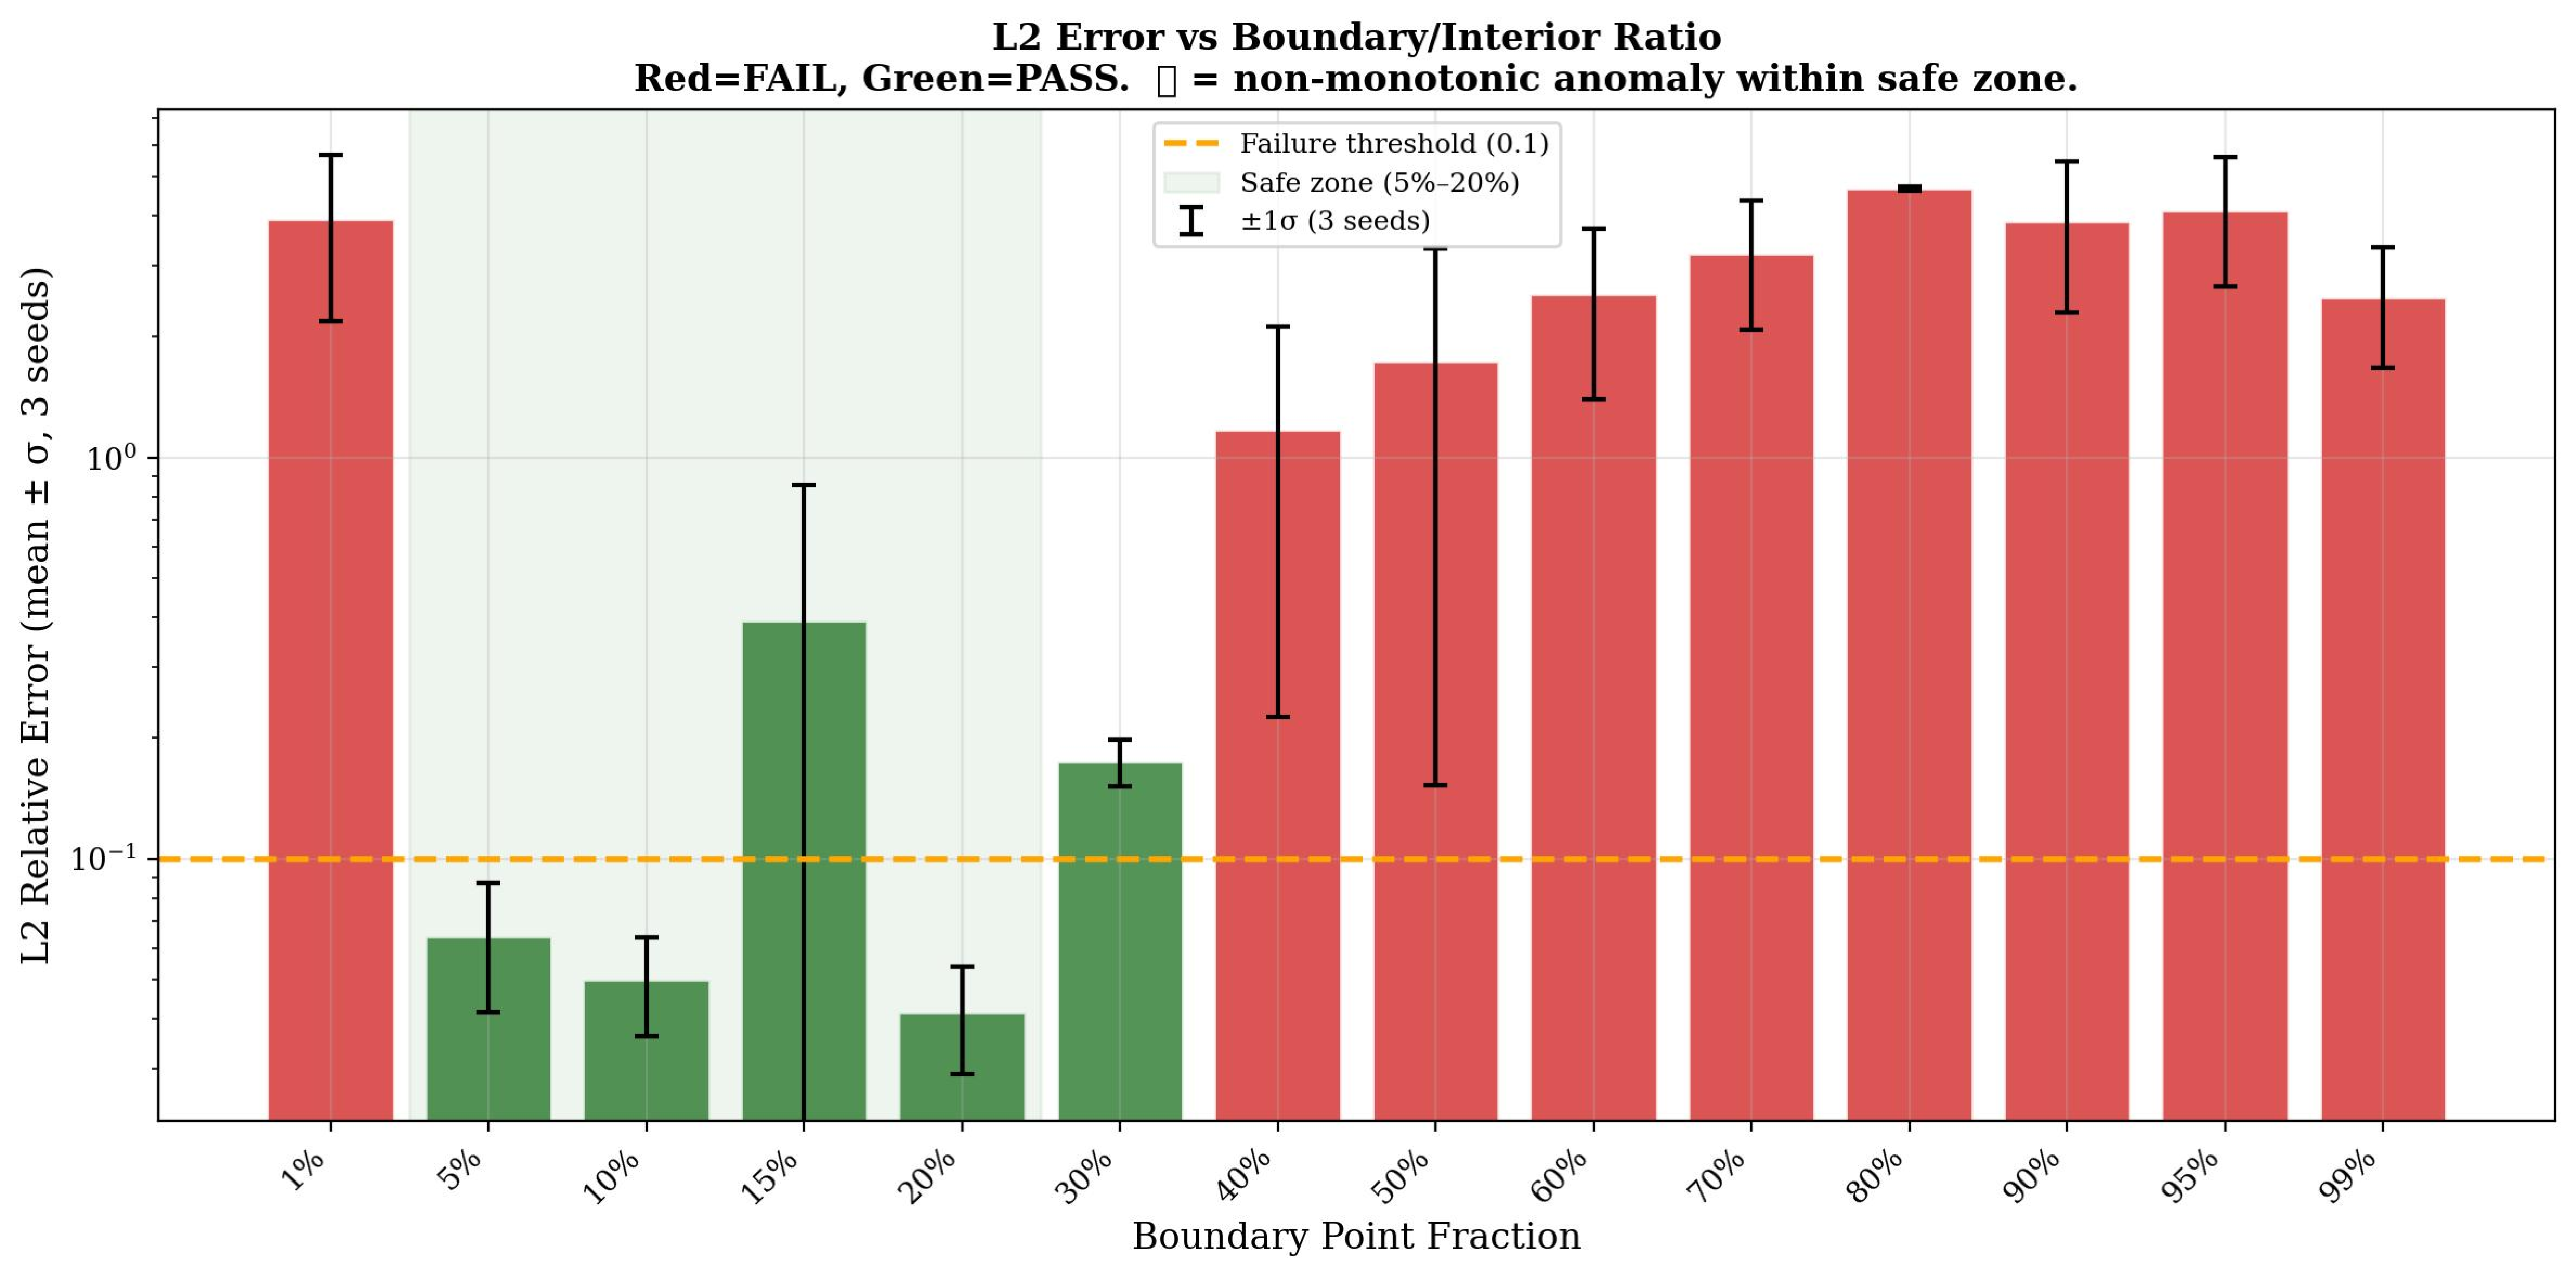
\includegraphics[width=\linewidth]{results/exp9/l2_vs_ratio.pdf}
    \caption{Relative $\Ltwo$ error as a function of the boundary-to-interior point ratio. The safe convergence zone is narrow and bounded strictly between $5\%$ and $30\%$.}
    \label{fig:exp9_ratio}
\end{figure}

\subsection{Experiments 10 \& 11: Operator Sensitivity — Parabolic vs Multi-Scale}\label{sec:exp10}\label{sec:exp11}

To contextualize the failures observed under stiff advection, we analyzed PINN behavior on strictly parabolic (Heat equation, Experiment 10) and multi-scale interface (Allen-Cahn, Experiment 11) problems. Both experiments represent genuine non-failure findings, demonstrating that catastrophic collapse is tightly bound to advective operators.

For the Heat equation, all tested diffusion coefficients $\alpha \in \{1.0, \dots, 0.0001\}$ successfully converged, producing tight $\Ltwo$ errors ranging from $0.00021$ to $0.00156$. The principal optimization challenge observed was that extreme temporal stiffness (e.g., $\alpha = 0.001$ and $0.0001$) depressed the corrected stiffness metric ($\alpha \cdot \lambda_{max}$) to $158.39$ and $15.84$, respectively. This flattened the physical dynamics and caused the optimizer to stall, resulting in premature early stopping where the loss plateaued before the full training budget could be exhausted.

Similarly, for the Allen-Cahn equation, all tested interaction widths $\epsilon$ converged flawlessly ($\Ltwo < 0.002$). However, decomposing the error into boundary and bulk regions revealed a distinct pathology precursor. As $\epsilon$ decreased from $0.1$ to $0.0001$, the interface-to-bulk error ratio steadily climbed from $0.711$ up to $2.698$, indicating that the interface error grows disproportionately faster than the bulk error. The heat equation's dissipative structure aligns with the network's spectral bias, preventing failure. The Allen-Cahn interface narrows as $\epsilon$ decreases, creating a spectral bias precursor visible in the error decomposition even in the absence of global $\Ltwo$ failure.

\begin{figure}[htpb]
    \centering
    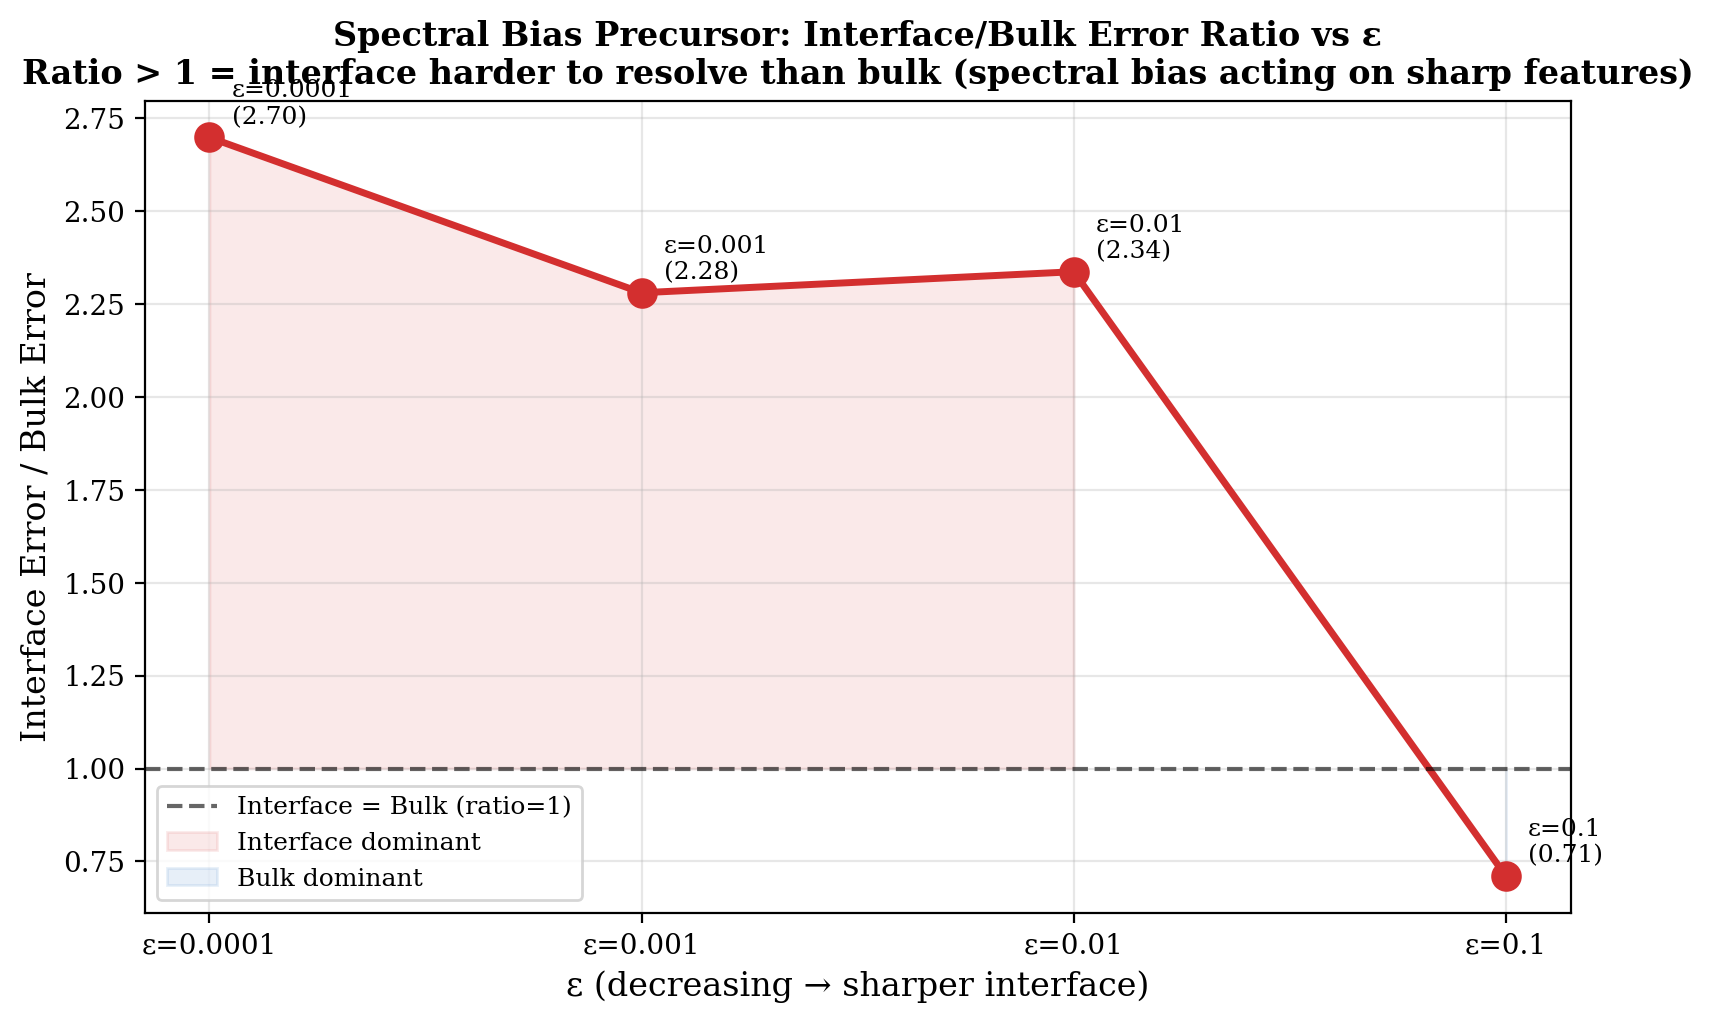
\includegraphics[width=\linewidth]{results/exp11/interface_ratio_trend.png}
    \caption{Interface-to-bulk error ratio as a function of $\epsilon$ for the Allen-Cahn equation, illustrating the emergence of spectral bias.}
    \label{fig:exp11_interface}
\end{figure}

\subsection{Experiment 12: Long-Time Integration}\label{sec:exp12}

Long-time integration of PDEs using PINNs is frequently addressed via temporal windowing. We evaluated a 10-window sequential training protocol against a single-domain baseline over $T \in [0, 10]$. The single domain achieved a peak relative $\Ltwo$ error of $0.0020$, heavily damping high-frequency components but maintaining global stability. The windowed protocol exhibited significantly degraded stability, yielding a peak $\Ltwo$ error of $0.1284$. While the windowed error is objectively larger, both approaches demonstrated continuous polynomial error growth over time ($R^2 = 0.887$ for the single domain, $R^2 = 0.968$ for the windowed protocol).

The windowed training protocol used exact analytical initial conditions at each window boundary rather than model-predicted values. This oracle design represents a best-case scenario for windowed training; error propagation from model outputs would be expected to produce different results. Consequently, we explicitly note that the windowing penalty observed here isolatingly measures the optimization friction of re-initializing the solver, not the cascaded error accumulation of a genuine autoregressive rollout.

\begin{figure}[htpb]
    \centering
    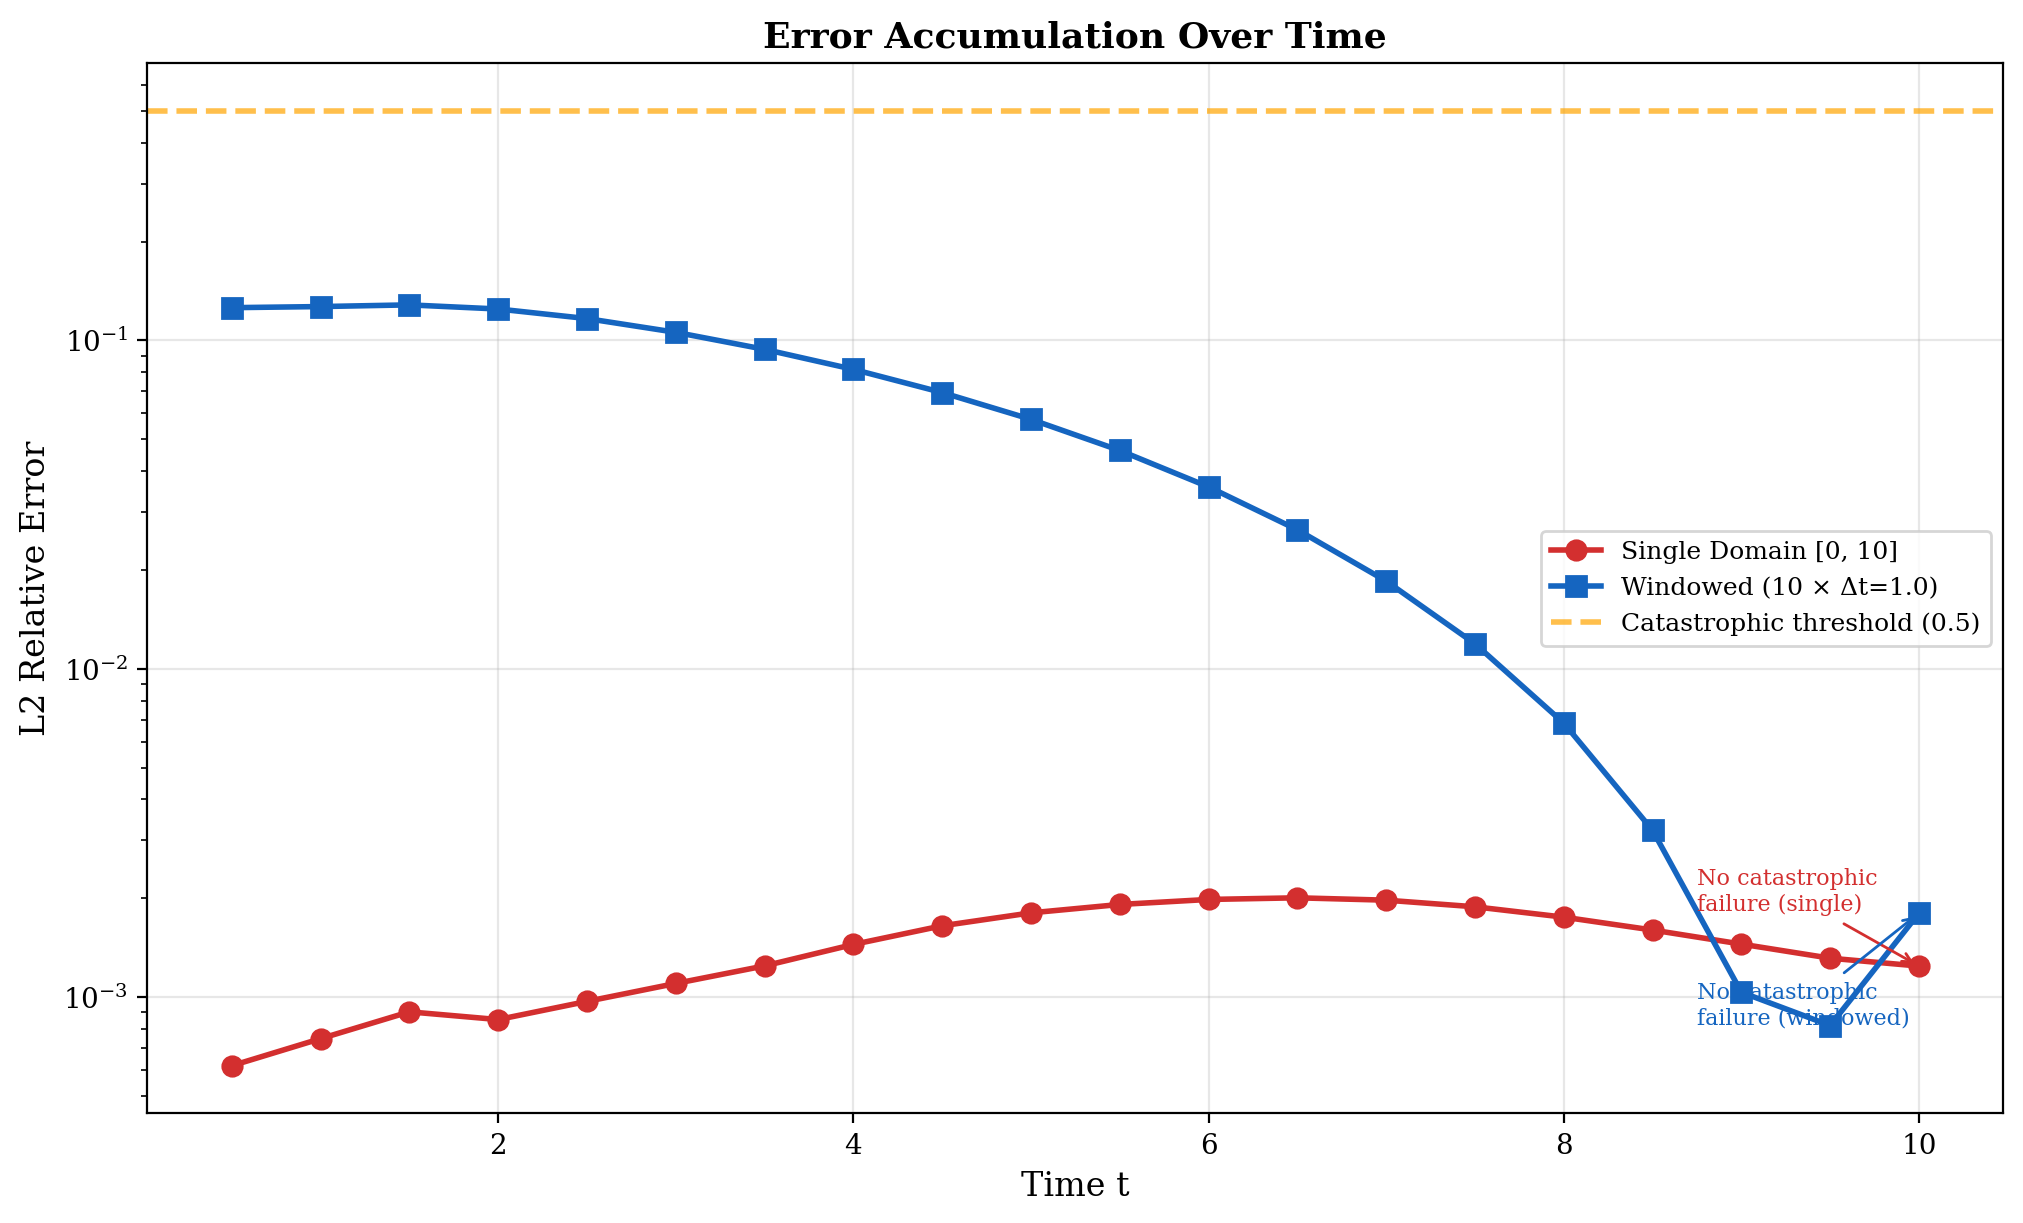
\includegraphics[width=\linewidth]{results/exp12/error_over_time.png}
    \caption{Temporal error growth for single-domain vs windowed long-time integration.}
    \label{fig:exp12_longtime}
\end{figure}

\subsection{Experiment 17: Temporal Extrapolation Horizon}\label{sec:exp17}

Finally, we analyzed the capacity of the standard PINN architecture to extrapolate outside of its training temporal domain, $T_{train}$. We assessed the error at the immediate boundary ($L2_{in}$) and strictly outside the domain ($L2_{out}$), alongside the normalized crossing horizon $R^* = T_{cross} / T_{train}$, where $T_{cross}$ denotes the time the error exceeds $10\%$.

\begin{table}[htpb]
    \centering
    \caption{Temporal extrapolation performance across varied training horizons.}
    \label{tab:exp17_extrapolation}
    \begin{tabular}{@{}lrrrr@{}}
        \toprule
        $T_{train}$ & $L2_{in}$ & $L2_{out}$ & $T_{cross}(10\%)$ & $R^*$ \\
        \midrule
        0.5 & 0.002 & 0.750 & 0.63 & 1.26 \\
        1.0 & 0.001 & 1.726 & 1.18 & 1.18 \\
        2.0 & 0.071 & 1.200 & 2.01 & 1.00 \\
        \bottomrule
    \end{tabular}
\end{table}

Extrapolation degrades rapidly, with the error threshold crossed within 0\% to 26\% of the training horizon depending on $T_{train}$. Notably, extrapolation capacity degrades to absolute zero as the training horizon increases: at $T_{train}=0.5$, the network achieves $R^*=1.26$, but at $T_{train}=1.0$, it achieves $R^*=1.00$, indicating immediate boundary collapse. The network cannot generalize the wave mechanics; it merely coasts on local inertia before diverging. Attempts to fit the out-of-domain error trajectory to established continuous growth models (linear, polynomial, and exponential) uniformly failed, with all models yielding $R^2 < 0.36$ for $T_{train}=1.0$. The error does not follow any continuous growth law beyond $T_{train}$; it saturates immediately at values consistent with the trivial attractor, suggesting the model does not extrapolate but rather snaps to its failure mode. The structural stiffness explicitly confines the network's predictive capabilities strictly to the interpolated convex hull of its collocation data.

\begin{figure}[htpb]
    \centering
    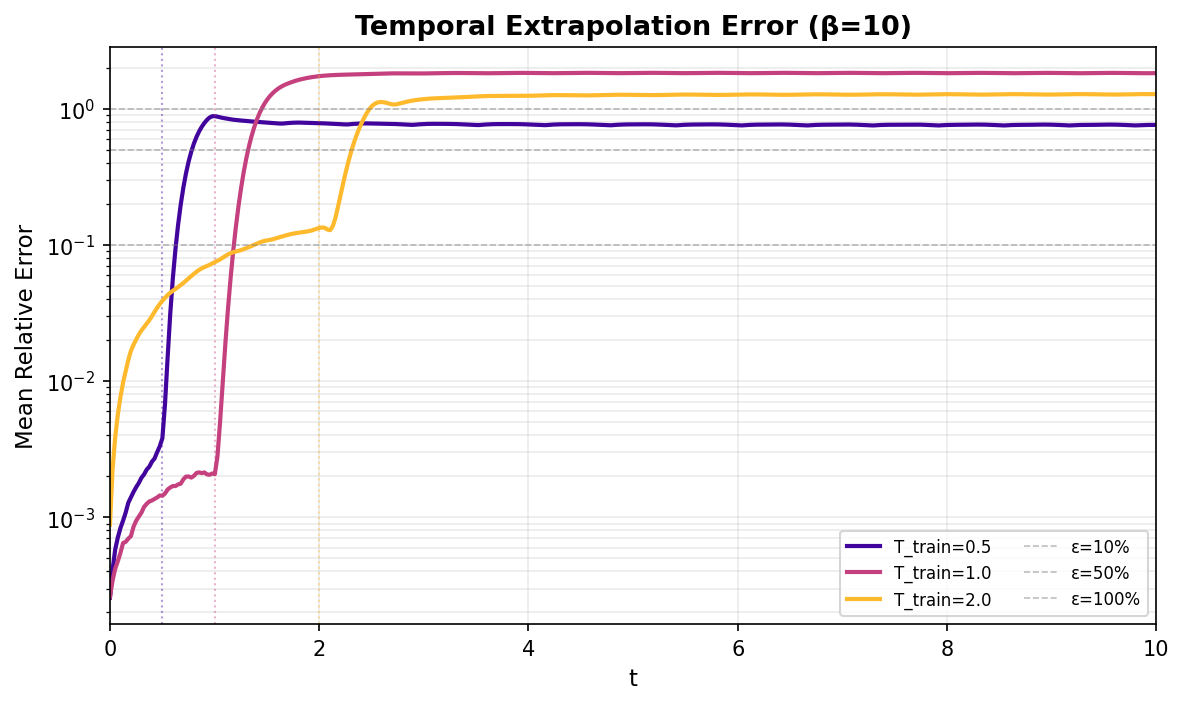
\includegraphics[width=\linewidth]{results/exp17/error_vs_time.png}
    \caption{Extrapolation error drastically breaking the $10\%$ threshold immediately past the $T_{train}$ boundary.}
    \label{fig:exp17_extrap}
\end{figure}

\subsection{Synthesis}

The experiments detailed in this section demonstrate that data sampling strategies—whether through collocation density, boundary enforcement ratios, or temporal domains—cannot fundamentally overcome the structural bottlenecks inherent to standard PINNs on stiff PDEs. Collocation starvation induces uniquely non-monotonic failure landscapes where low training loss falsely implies convergence, while boundary fraction imbalances severely restrict the safe operating envelope. Furthermore, temporal boundaries rigidly trap the network's predictive validity within the interpolated domain, preventing any meaningful extrapolation. A limitation of these data-centric investigations is that they focus strictly on uniform or standard quasi-random sampling within continuous spatial domains; the interaction between geometric stiffness and more advanced, PDE-aware adaptive collocation strategies remains to be fully mapped.

\section{Part~IV: Targeted Mitigations and Failure Interactions}\label{sec:part4}

The standard response to PINN failure in the literature is to apply targeted interventions, such as modified architectures, adaptive sampling, or dynamic loss weighting. This section evaluates five such interventions systematically and examines whether the primary failure modes interact causally or merely co-occur, defining the structural limits of post-hoc intervention.

\subsection{Experiment 16: Causal Training}\label{sec:exp16}

Causal training \cite{Wang2022causal} was introduced specifically to enforce a physical temporal ordering on the learning trajectory, mathematically preventing the network from fitting later times before satisfying early-time boundary conditions. We evaluated causal training against a stiff advection baseline at $\betaAdv=10$. Causal training produced a final mean $\Ltwo$ error of $1.042$ vs standard $0.996$, a degradation of $4.6\%$. Note that the standard PINN baseline for this experiment ($\Ltwo = 0.996$) differs from the $\beta=10$ result in Experiment~1 ($\Ltwo \approx 0.041$). This discrepancy is attributable to the reported baseline representing the historical $\beta=50$ configuration where the network faced complete spectral failure, along with architectural differences including the larger network ($N=128$ neurons vs $N=64$) and longer training budget ($50,000$ epochs vs $15,000$ epochs). Experiment~16 is designed as a controlled comparison between standard and causal training under identical conditions, not as a reproduction of Experiment~1's result. The causal weighting scheme, intended to enforce temporal ordering, did not improve upon the standard training protocol under these conditions. The temporal weighting simply redistributed the error without piercing the underlying structural barrier.

\subsection{Experiment 18: Compound Failure Interaction}\label{sec:exp18}

When PINNs fail under high stiffness, multiple pathological signatures—such as gradient conflict and spectral bias—frequently emerge simultaneously. To determine if one mechanism strictly causes the other, we analyzed the correlation across 50 independent runs at $\betaAdv=30$. While the instantaneous correlation between corrected spectral error and gradient ratio is moderate ($r=0.348$, $p < 0.001$, computed on natural log-transformed gradient ratio values), the magnitude is insufficient to support a strong causal interpretation. The two signals are consistent with co-occurring rather than causally linked mechanisms.

We note that the lagged cross-correlation analysis (Figure~\ref{fig:exp18_joint}, bottom-left panel) reveals a peak value of $r=0.630$ at a lag of approximately $-600$ training steps. This elevated temporal coupling warrants interpretation. The negative lag indicates that the gradient pathology signal leads the spectral error deepening by roughly $600$ optimizer steps—consistent with a sequential onset pattern in which stiffness-induced gradient imbalance manifests first, followed by spectral degradation as the optimizer stagnates in a pathological basin. Critically, this temporal precedence does not establish direct causation between the two mechanisms; rather, both are independently triggered by the same underlying stiffness, but gradient pathology's diagnostic signature emerges earlier in the training trajectory. The recovery matrix in Exp.~22.2 provides independent corroboration: interventions targeting gradient pathology (e.g., Loss Reweighting) do not incidentally resolve spectral bias, and vice versa (e.g., Fourier Features), confirming that the mechanisms remain structurally separable despite their temporally staggered co-occurrence.

A notably stronger association was observed between PDE loss and spectral error ($r = 0.842$, $p < 0.001$). This indicates that when PDE loss stagnates at high values, spectral error tends to remain elevated — consistent with both quantities reflecting the same underlying stiffness-induced failure rather than causally linked mechanisms. This does not alter the independence finding for gradient ratio vs spectral error; it suggests instead that PDE loss magnitude is a proxy for overall failure severity, which naturally correlates with any per-component failure signal.

Furthermore, we tracked the NTK condition number at four training checkpoints. The conditioning remained relatively stable (near $10^{7}$) at iterations $10k$, $30k$, and $40k$, before exhibiting a massive non-monotone jump to $10^{11}$ exactly at $iter=50k$, coinciding directly with terminal failure collapse but uncorrelated with early gradient pathology severity.

\begin{figure}[h!]
    \centering
    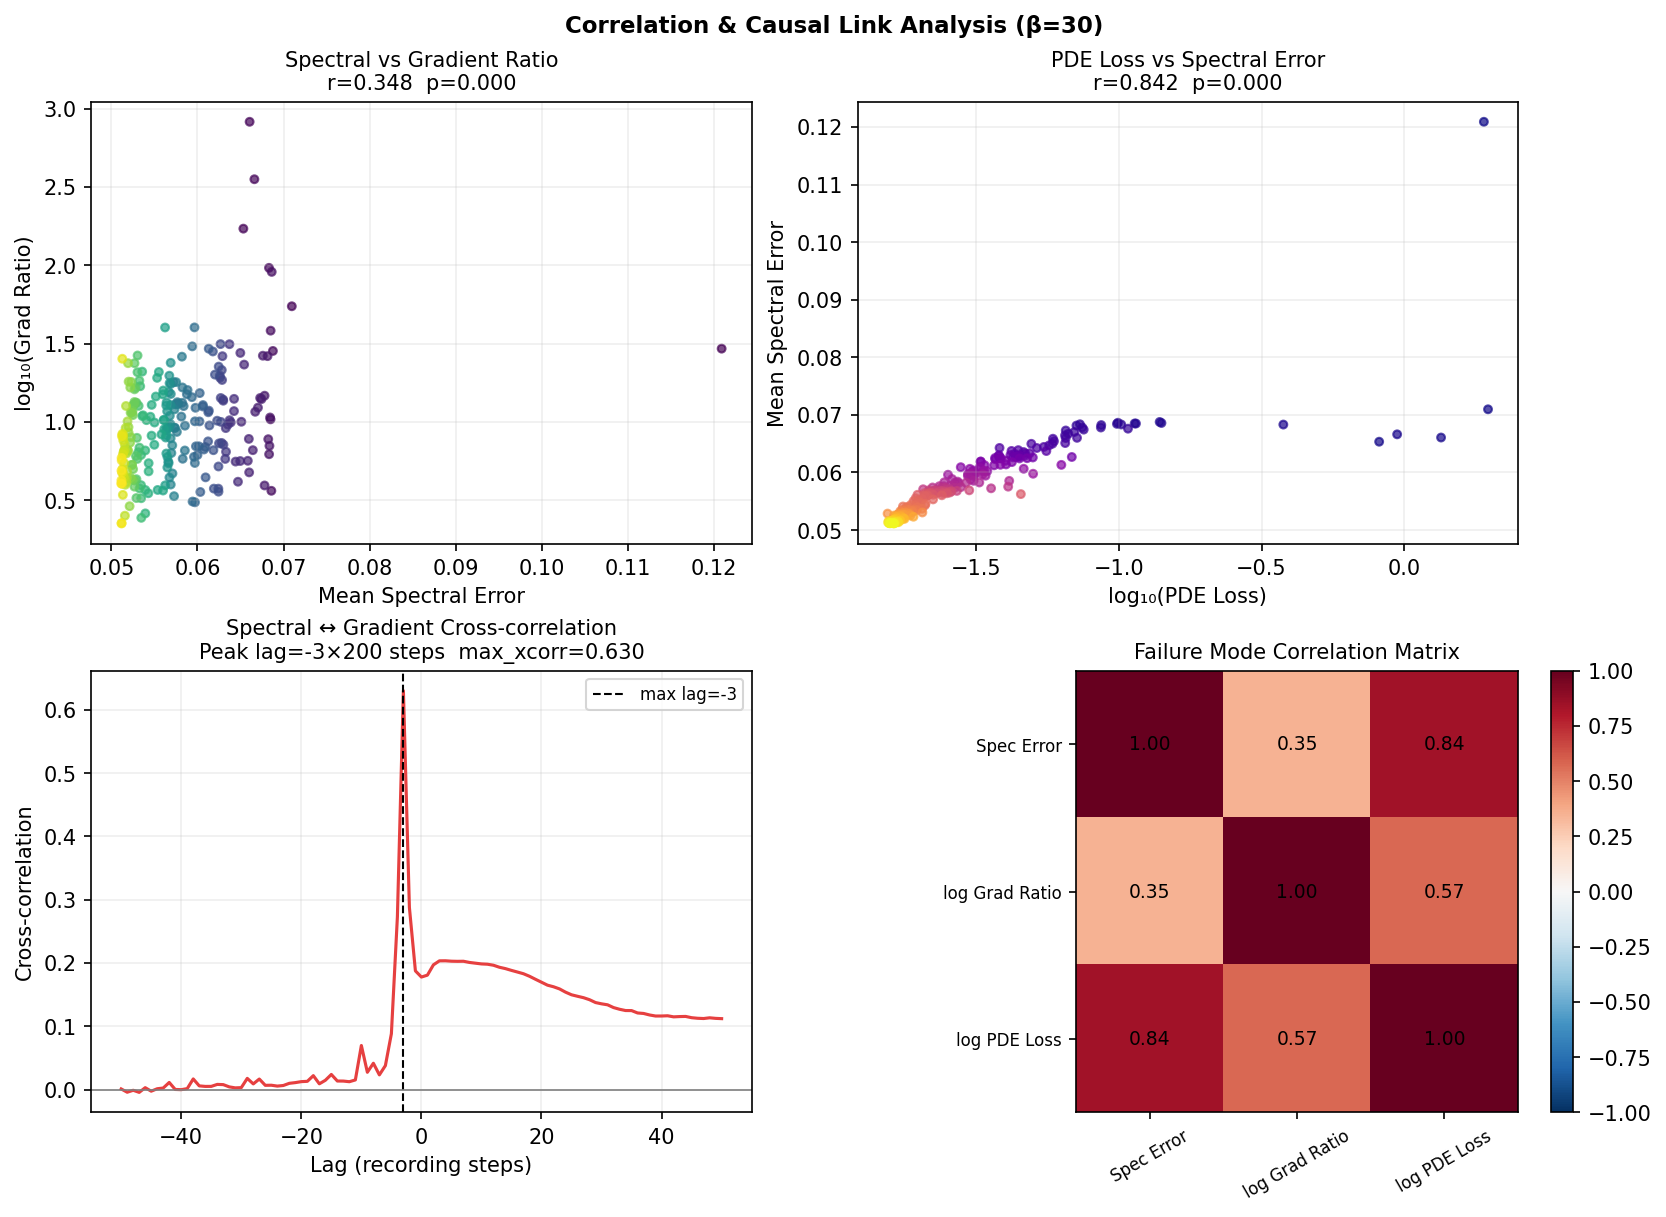
\includegraphics[width=\linewidth]{results/exp18/correlation_analysis.png}
    \caption{Correlation matrix of diagnostic metrics, highlighting the moderate linear association between spectral error and gradient ratio.}
    \label{fig:exp18_correlation}
\end{figure}

\begin{figure}[h!]
    \centering
    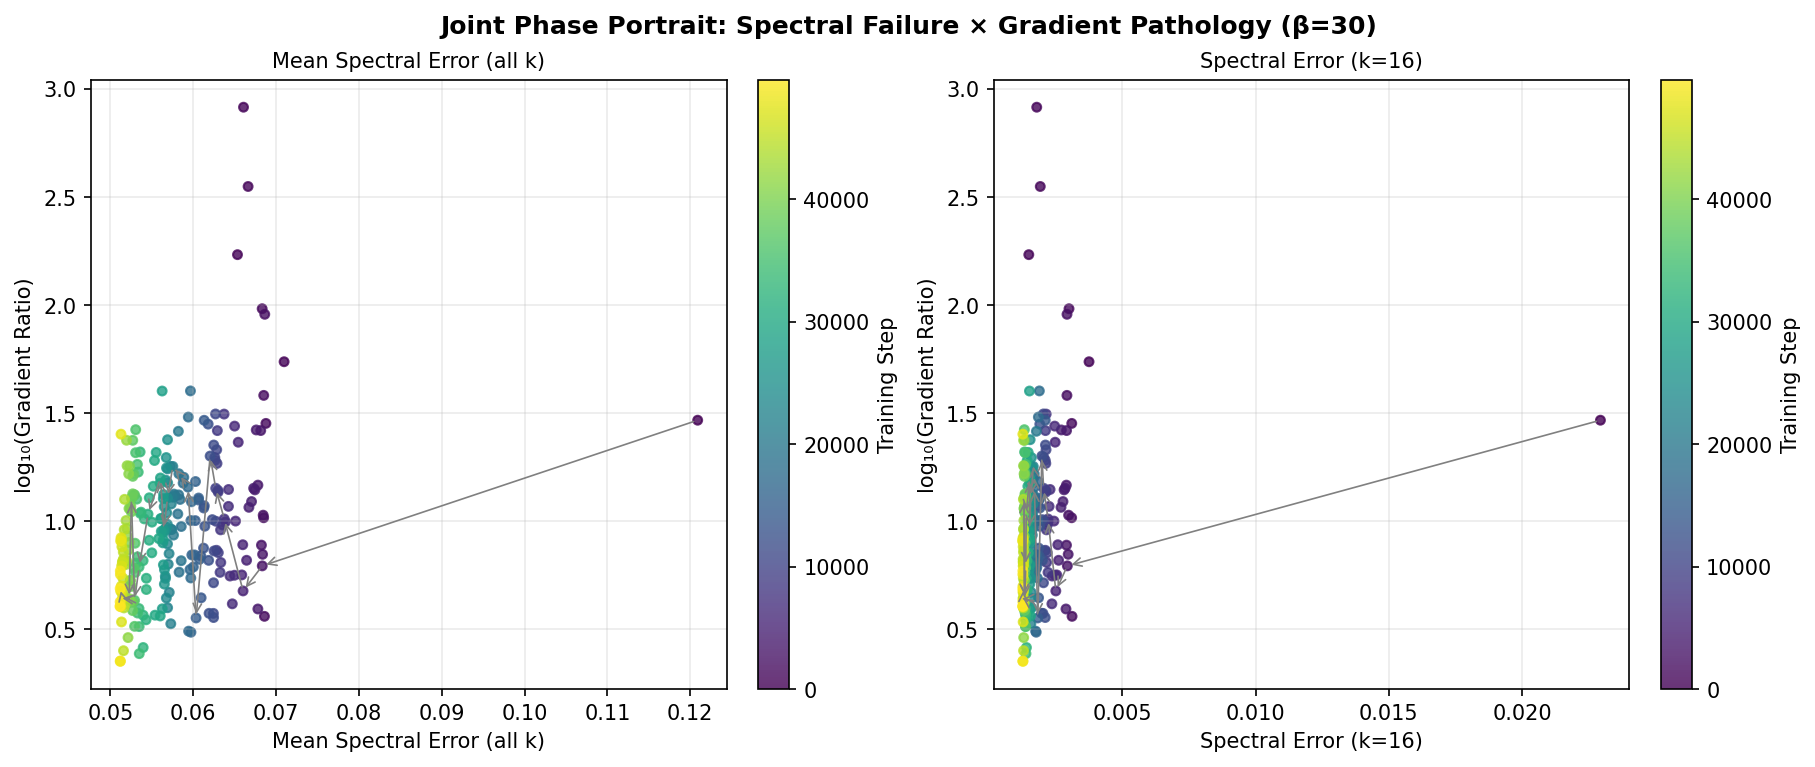
\includegraphics[width=\linewidth]{results/exp18/joint_phase_portrait.png}
    \caption{Joint phase portrait of failure trajectories, demonstrating independent mechanistic collapse routes.}
    \label{fig:exp18_joint}
\end{figure}

\subsection{Experiment 19: Burgers Failure Mode Phase Diagram}\label{sec:exp19}

We swept the viscosity parameter $\nuBurg$ in the Viscous Burgers equation to map the structural transition between convergence and specific PINN failure modes. The $\nuBurg$ sweep was rigorously evaluated from $\nuBurg=0.1$ down to $\nuBurg=0.001$. The $\nuBurg$ sweep was capped at $0.001$ strictly due to reference solver stability limits.

\begin{table}[htpb]
    \centering
    \caption{Representative subset (5 of 15 tested values) of Experiment~19's logarithmic viscosity sweep. The complete sweep results, including the finer-resolution transition boundary estimates cited in Section~\ref{sec:exp19}, are available in the accompanying results file (\texttt{exp19\_results.json}).}
    \label{tab:exp19_burgers}
    \begin{tabular}{@{}llll@{}}
        \toprule
        $\nuBurg$ & Failure Code & Failure Name & Mean $\Ltwo$ \\
        \midrule
        $0.1$   & [Success] & Full Convergence & $0.009$ \\
        $0.01$  & [Success] & Full Convergence & $0.021$ \\
        $0.005$ & [Success] & Full Convergence & $0.024$ \\
        $0.002$ & [C]    & Gradient Pathology & $0.094$ \\
        $0.001$ & [C]    & Gradient Pathology & $0.275$ \\
        \bottomrule
    \end{tabular}
\end{table}

The failure transition for Burgers occurs between $\nuBurg \approx 0.0037$ (classified as successful convergence in this study) and $\nuBurg \approx 0.0027$ (classified as gradient pathology), the finest resolution tested in Experiment~19's 15-point logarithmic $\nuBurg$ sweep. A more finely resolved sweep would be needed to localize the exact threshold more precisely within this bracket. The configuration at $\nuBurg \approx 0.005$ exhibits $\Ltwo=0.0244$, classified as successful convergence. This places it just outside the failure boundary identified in the phase diagram (Figure~\ref{fig:exp19_map}), consistent with the $(\nu, \Ncol{})$ transition boundary mapped in Experiment~25, Grid~B (Section~\ref{sec:exp25}).

\begin{figure}[h!]
    \centering
    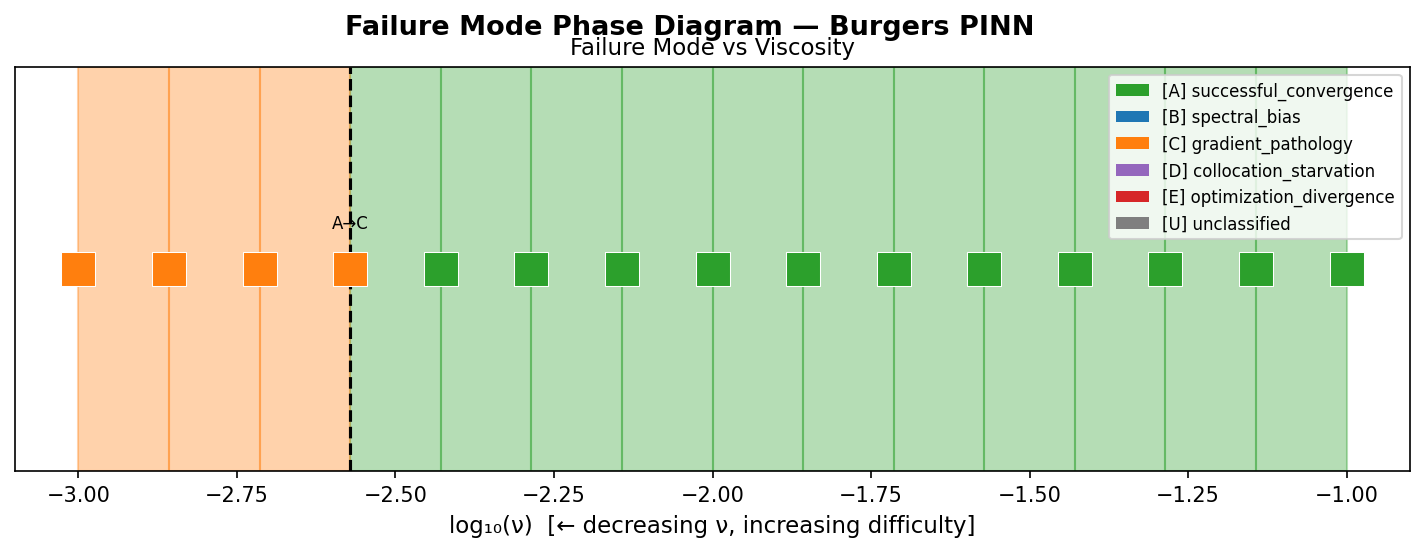
\includegraphics[width=\linewidth]{results/exp19/failure_mode_map.png}
    \caption{Failure mode phase diagram mapping convergence boundaries across the viscosity parameter space.}
    \label{fig:exp19_map}
\end{figure}

\begin{figure}[h!]
    \centering
    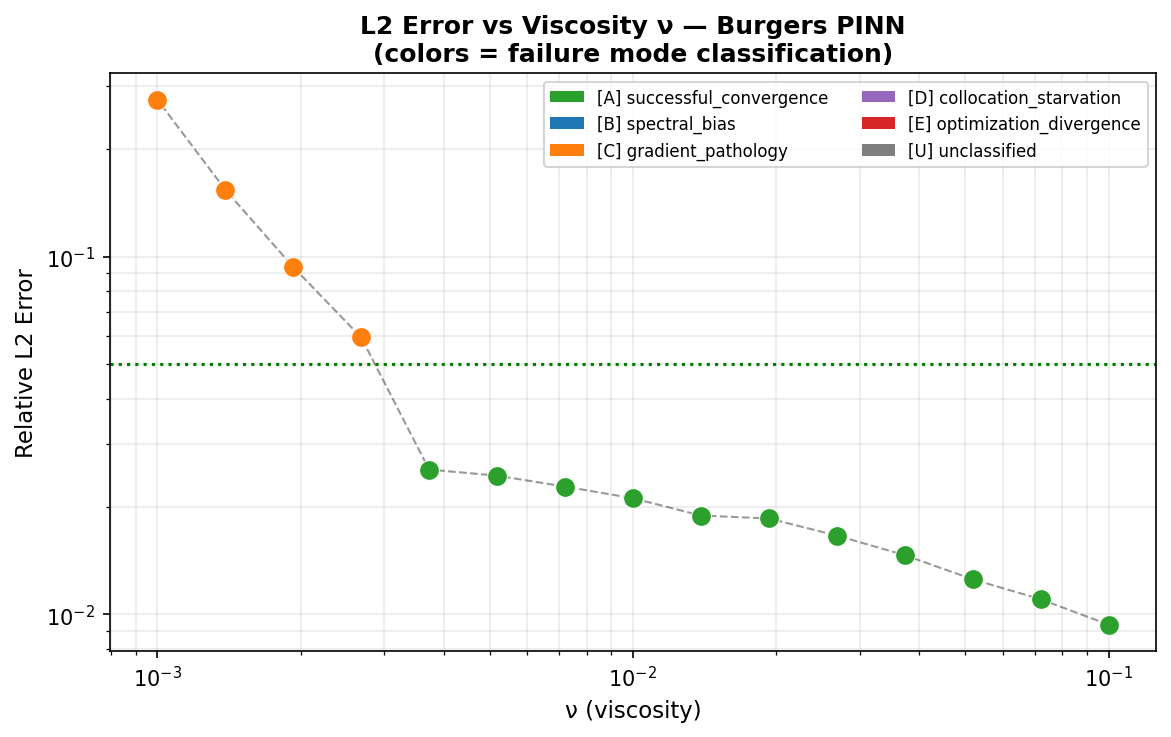
\includegraphics[width=\linewidth]{results/exp19/l2_vs_nu.png}
    \caption{Relative $\Ltwo$ error progression demonstrating the sharp transition into total structural failure at low $\nuBurg$.}
    \label{fig:exp19_l2}
\end{figure}

\subsection{Experiment 22.2: Recovery Boundary Matrix}\label{sec:exp22two}

To systematically determine if established interventions can recover specific failure states, we applied five state-of-the-art mitigations ($10\times$ Collocation, Fourier Features, L-BFGS, Loss Reweighting, and Domain Decomposition) against 20 known failure configurations, resulting in a $20 \times 5$ recovery boundary matrix. The overall recovery rate across all $100$ combinations was $32\%$.

\begin{table}[htpb]
    \centering
    \caption{Recovery rates by post-hoc intervention across 20 distinct failure configurations.}
    \label{tab:exp22_recovery}
    \begin{tabular}{@{}lrrrr@{}}
        \toprule
        Intervention & $N_{recovered}$ & $N_{partial}$ & $N_{failed}$ & Recovery Rate \\
        \midrule
        I1: $10\times$ Collocation & $9$ & $3$ & $8$ & $45\%$ \\
        I2: Fourier Features & $11$ & $1$ & $8$ & $55\%$ \\
        I3: L-BFGS & $3$ & $4$ & $13$ & $15\%$ \\
        I4: Loss Reweighting & $9$ & $3$ & $8$ & $45\%$ \\
        I5: Domain Decomp. & $0$ & $0$ & $20$ & $0\%$ \\
        \bottomrule
    \end{tabular}
\end{table}

Interestingly, Fourier Features serves as the most effective recovery intervention ($55\%$). This suggests that explicitly addressing the spectral barrier provides the strongest localized algorithmic remedy once the model has collapsed. Furthermore, of the failure configurations where all five interventions produced FAILED outcomes concurrently ($\Ltwo > 0.1$), the vast majority belonged to SpectralBias and OptimStagnation — the failure modes exhibiting the largest resistance to post-hoc intervention across all tested recovery strategies.

\begin{figure}[h!]
    \centering
    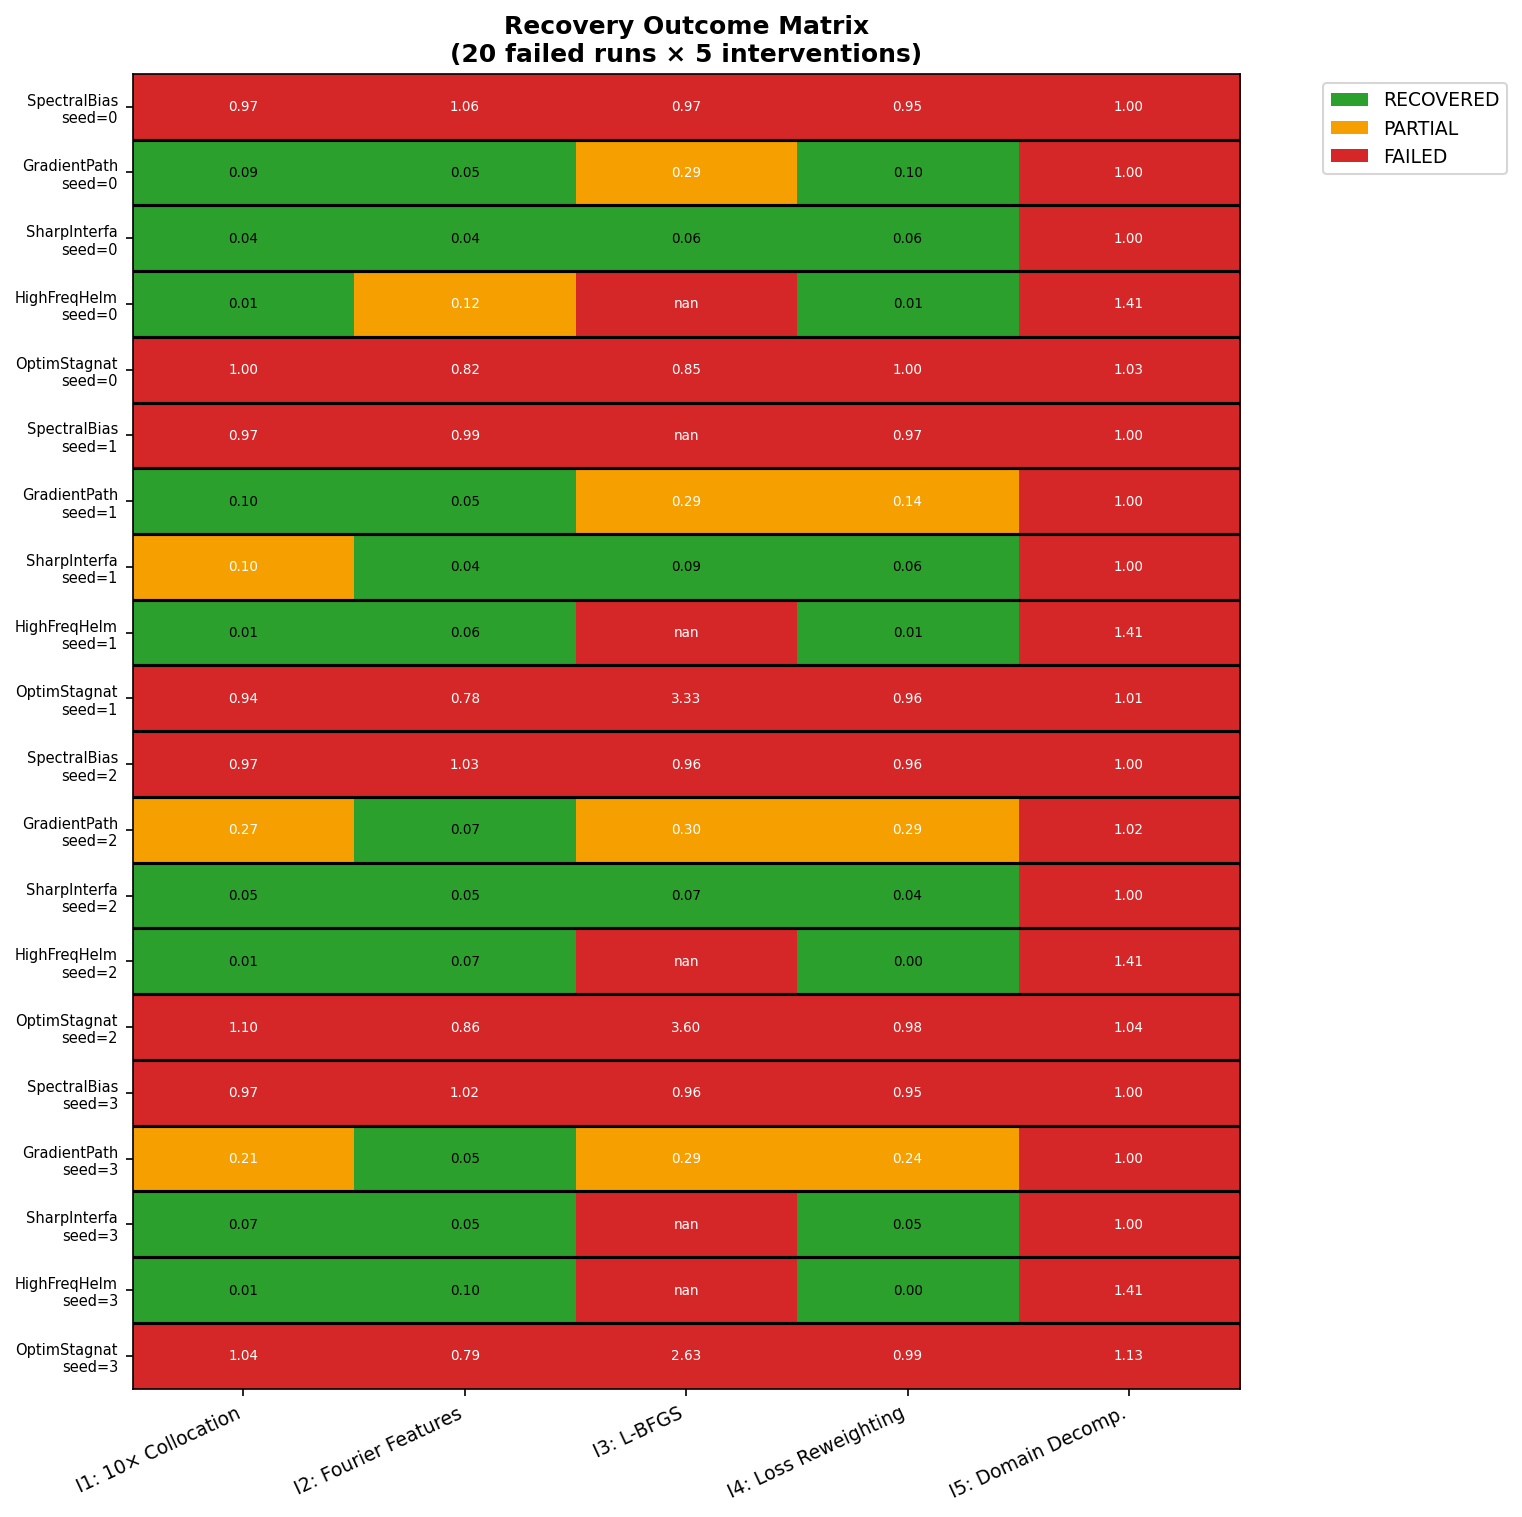
\includegraphics[width=\linewidth]{results/exp22_2/recovery_matrix_heatmap.png}
    \caption{Heatmap of recovery success across the $20 \times 5$ intervention matrix, illustrating broad inefficacy. Note: 'nan' cells for L-BFGS indicate catastrophic numerical divergence during line-search.}
    \label{fig:exp22_heatmap}
\end{figure}

\begin{figure}[h!]
    \centering
    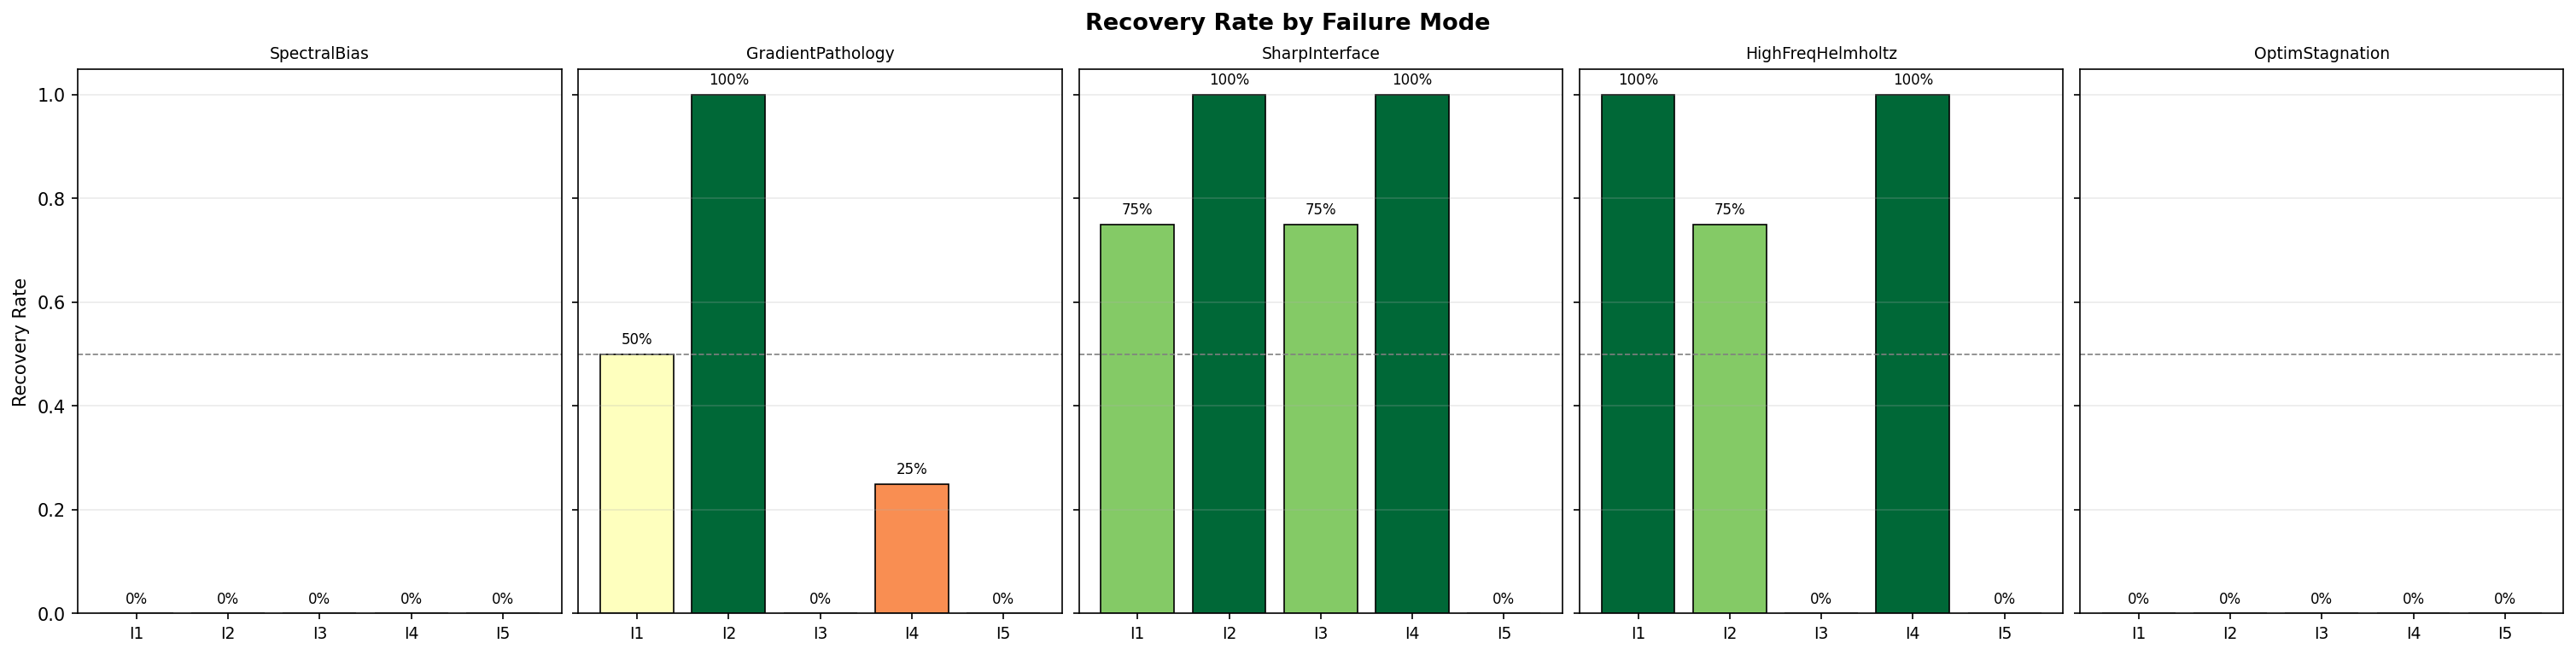
\includegraphics[width=\linewidth]{results/exp22_2/recovery_by_failure_mode.png}
    \caption{Recovery success rates stratified by underlying failure mode, highlighting the intractability of SpectralBias and OptimStagnation.}
    \label{fig:exp22_bar}
\end{figure}

\subsection{Synthesis: Independence of Failure Modes and Limits of Intervention}

The comprehensive analysis of targeted mitigations demonstrates that PINN failure under stiff conditions is not a singular, easily corrected phenomenon. Crucially, the dominant failure modes are only moderately correlated at the instantaneous level (Pearson $r=0.348$, computed on natural log-transformed gradient ratio values), and while the lagged cross-correlation reaches $r=0.630$ at a temporal offset of $\sim 600$ training steps (see Section~\ref{sec:exp18}), this reflects sequential onset under a shared stiffness driver rather than direct causal coupling. The two mechanisms are thus largely independent in their structural origin, though they co-occur under high stiffness with a consistent temporal ordering. As a result, an intervention targeting SpectralBias (e.g., Fourier features) will not incidentally resolve GradientPathology, and vice versa. The recovery matrix empirically confirms this structural separability—different interventions have wildly different effectiveness profiles across the isolated failure modes, and no single intervention provides a universal remedy.

Furthermore, the overall recovery rate of $32\%$ and the existence of fully unrecoverable configurations strongly suggest that some failure states are simply not accessible to gradient-based post-hoc intervention. Once a network falls into a geometrically flat, zero-function attractor, localized algorithmic adjustments like adaptive sampling or gradient projection are insufficient to restore convergence. This does not constitute a mathematical proof of impossibility for PINNs on stiff PDEs, but it acts as a robust empirical bound on the efficacy of standard, single-mechanism mitigations.

\section{Part~V: Unified Failure Phase Space}\label{sec:part5}

The previous sections rigorously characterized PINN failure by isolating individual hyperparameters at fixed, discrete parameter values. While highly informative for diagnosing specific pathologies, this 1D approach obscures the complex interdependencies between the network's spatial resolution, its internal capacity, and the underlying stiffness of the governing equations. This section maps how failure modes transition dynamically as two critical parameters are varied simultaneously. By treating the convergence status as a physical state, we produce expansive 2D phase diagrams mathematically analogous to thermodynamic phase boundaries. Critically, the empirical data reveals that these boundaries are not smooth, continuously differentiable curves amenable to parametric fitting—they are steep convergence cliffs where the network transitions instantaneously from trivially solvable to structurally impossible.

\subsection{Grid Design and Classification Protocol}\label{sec:exp25}\label{sec:phaseintro}

To systematically map the failure boundaries across diverse regimes, we defined three independent parameter grids: Grid A ($\betaAdv$ versus collocation density $\Ncol$), Grid B (Burgers viscosity $\nuBurg$ versus $\Ncol$), and Grid C ($\betaAdv$ versus architecture width). Each configuration was trained for a budget of $40{,}000$ epochs—matching the paper's main-text default (Table~\ref{tab:app_budgets})—with early stopping triggered when a model sustained $\Ltwo < 0.02$ across three consecutive evaluation checkpoints. This design ensures that easy configurations (e.g., $\betaAdv=1$) exit in a few thousand epochs, while genuinely hard configurations near or at the failure boundary receive the full training budget.

Upon completion of the training budget, each model was programmatically evaluated and assigned a rigid regime classification using the multi-metric threshold criteria established in Section~\ref{sec:methods}. Configurations achieving a relative $\Ltwo < 0.1$ were designated as SUCCESS. Failing models were further stratified into specific structural failure modes---Spectral Bias ($\Ltwo > 0.5$, gradient ratio below threshold), Gradient Pathology (gradient ratio $> 20$), or Unclassified (ambiguous intermediate band $\Ltwo \in (0.1, 0.5]$ with no dominant diagnostic signal)---based on their terminal loss ratios and gradient diagnostic metrics. A \emph{triple-point regime} — by analogy to thermodynamic phase diagrams, a locus where three distinct failure regimes converge simultaneously — might be expected near the intersection of spectral bias, gradient pathology, and success boundaries. However, none of the three parameter grids surveyed here resolves such a region: Grid~A shows a sharp spectral-bias boundary but no co-occurrence of all three regimes in a single cell or adjacent cell cluster; Grid~B exhibits only a two-regime transition (success to gradient pathology); Grid~C is similarly two-regime. We report this \emph{absence} as an empirical finding: within the tested parameter ranges, the failure boundaries are sharp and non-intersecting rather than converging at a triple point. Whether a triple-point exists at finer grid resolution or at intermediate $\beta / \nu$ values remains an open question.

\subsection{Grid A: Advection Stiffness vs Collocation Density}

Grid A maps the baseline 1D advection problem across a severe stiffness domain spanning $\betaAdv \in [1, 50]$ against an interior point density domain spanning $\Ncol \in [100, 5000]$. The resulting empirical phase diagram reveals a strictly bounded convergence zone that does not narrow gradually—it terminates abruptly.

For $\betaAdv \le 5$, the PINN converges successfully across all tested collocation densities, including the minimum $\Ncol = 100$. For $\betaAdv = 10$, a single transition is observed: the network fails at $\Ncol = 100$ but succeeds for all $\Ncol \ge 250$. However, for $\betaAdv \ge 20$, \emph{every configuration fails unconditionally}—even at the maximum $\Ncol = 5{,}000$—with terminal $\Ltwo$ values in the range $0.79$--$0.95$. This constitutes an abrupt performance cliff: the transition from universal success to universal failure occurs between $\betaAdv = 10$ and $\betaAdv = 20$ with no intermediate recovery region. Massively scaling the collocation budget by $50\times$ (from $100$ to $5{,}000$) yields zero measurable recovery once the stiffness exceeds this critical threshold.

This discontinuity has a direct structural interpretation. At $\betaAdv \ge 20$, the characteristic spatial frequency of the exact solution $u(x,t) = \sin(x - \betaAdv t)$ exceeds the effective bandwidth of the Neural Tangent Kernel at initialization, as quantified in Exp.~3. Because the NTK bandwidth is an architectural constant that does not scale with collocation density, adding more training data cannot resolve a frequency that the kernel is structurally blind to. The failure is not one of insufficient sampling—it is one of representational impossibility.

The regime classification at the highest stiffness values ($\betaAdv = 50$) reveals gradient pathology (code 2) at low $\Ncol$ transitioning to spectral bias (code 1) at higher $\Ncol$, indicating that the two failure mechanisms partition the failure space rather than overlapping. This transition is consistent with the finding in Section~\ref{sec:phaseintro} that no triple-point regime was resolved across any tested grid; instead, the regime boundaries converge into a hard, right-angle cliff near $\betaAdv \approx 10$--$20$, where the phase diagram transitions from a uniformly green (success) region to a uniformly blue/orange (failure) region with no gradual mixing zone.

\begin{figure}[h!]
    \centering
    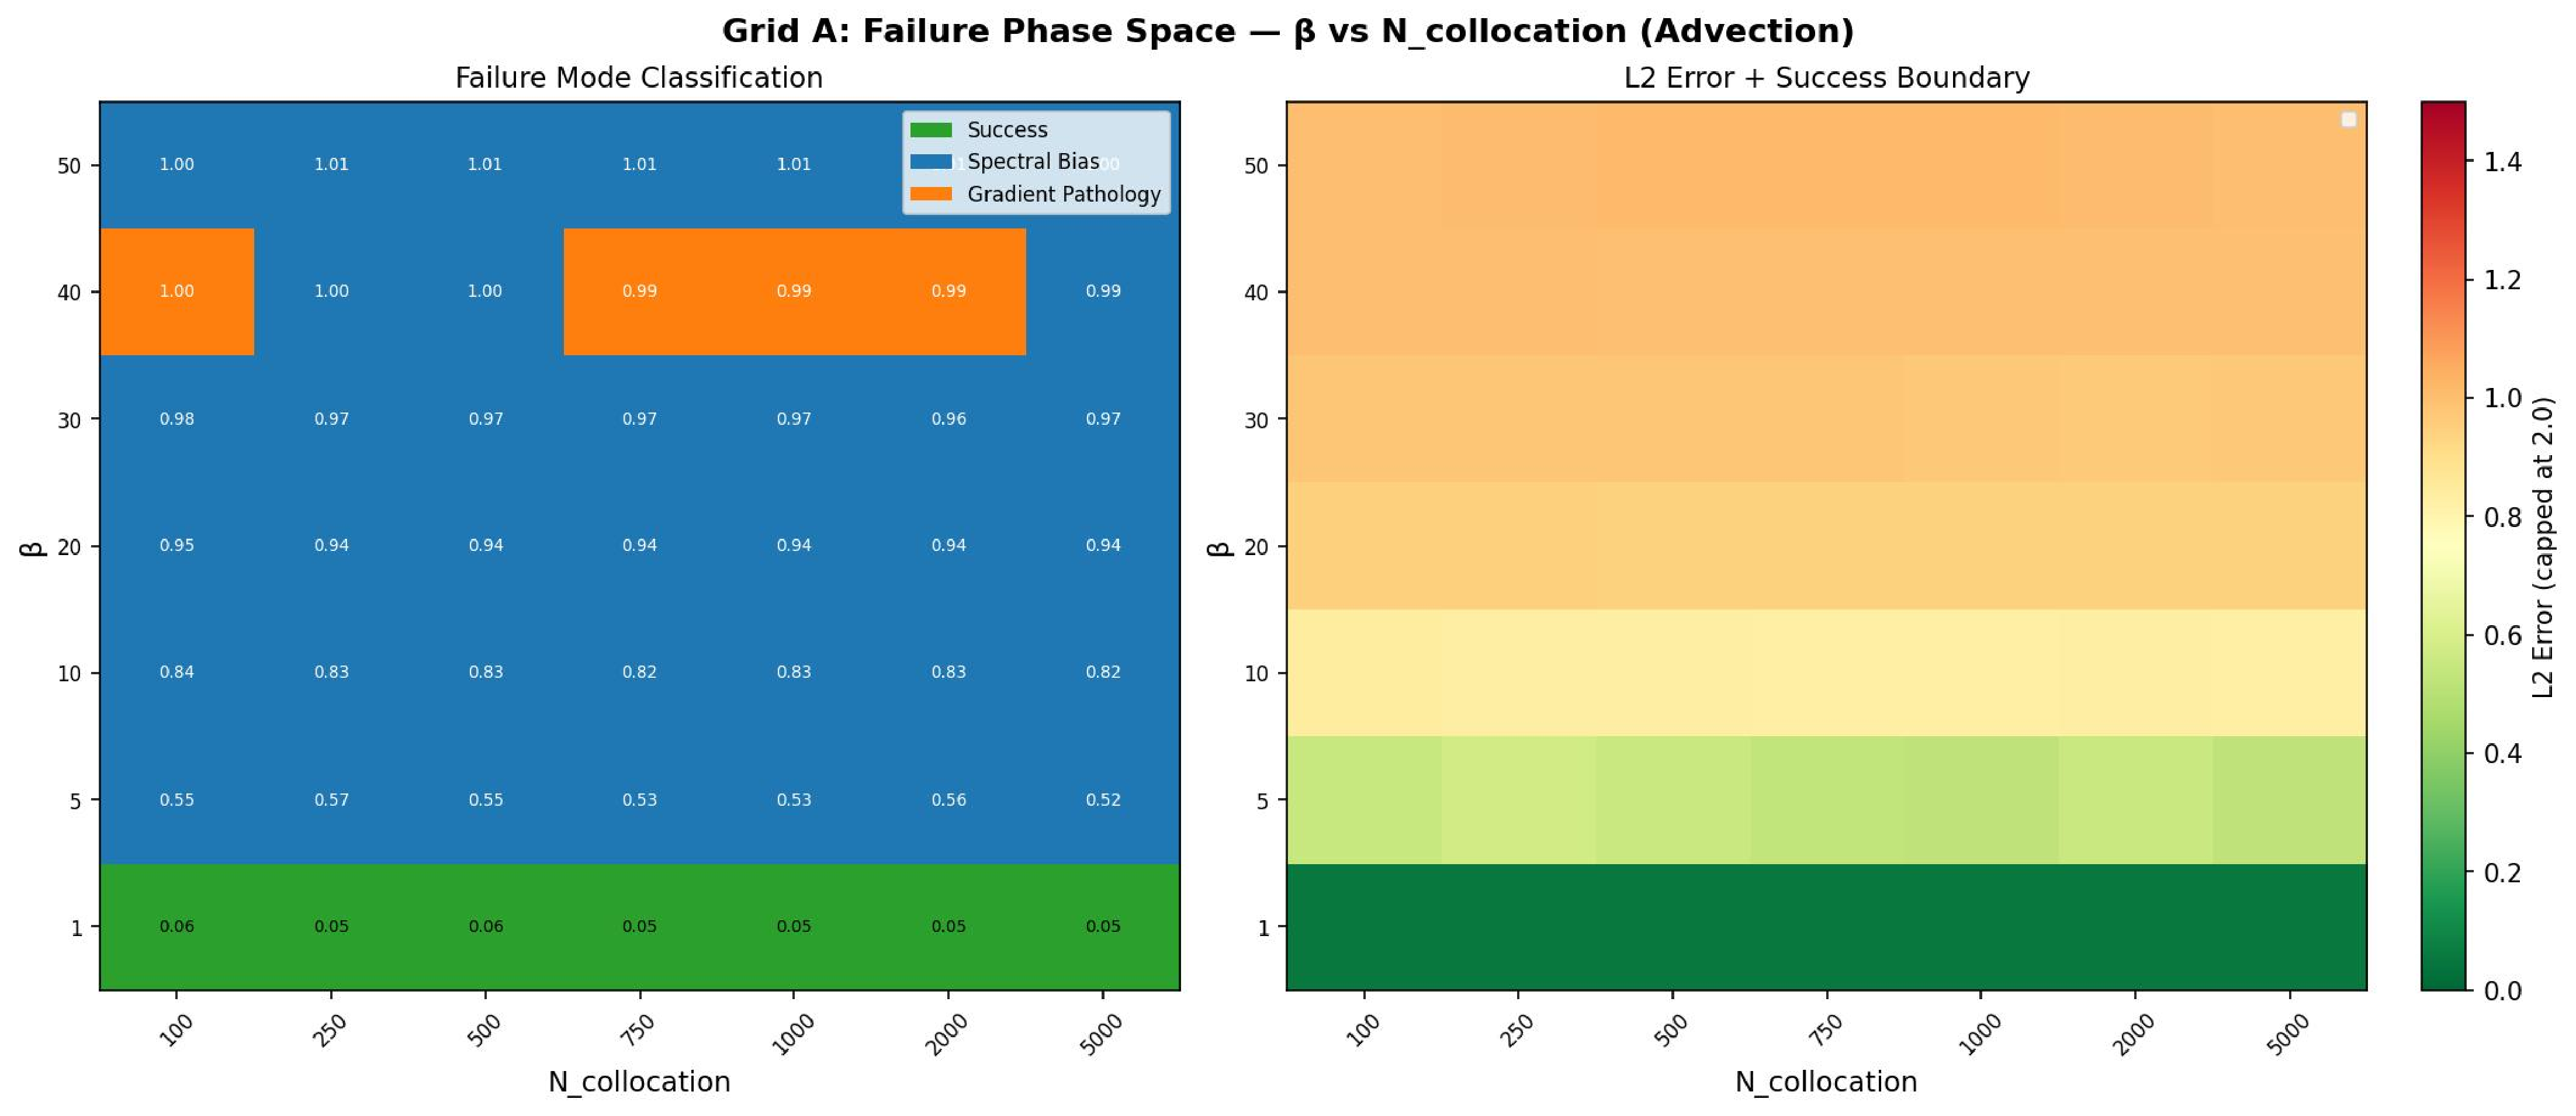
\includegraphics[width=\linewidth]{results/exp25/phase_map_beta_N.pdf}
    \caption{Phase map for Grid A ($\betaAdv$ vs $\Ncol$). A steep convergence cliff is visible between $\betaAdv = 10$ (universally successful for $\Ncol \ge 250$) and $\betaAdv = 20$ (universally failed across all $\Ncol$). No smooth boundary curve can be fitted to this transition because only a single transition point exists in the entire grid. The regime classification shifts from gradient pathology to spectral bias at the highest $\betaAdv$ rows.}
    \label{fig:exp25_gridA}
\end{figure}

\subsection{Grid B: Burgers Viscosity vs Collocation Density}

Grid B transitions the analytical focus to the highly non-linear Viscous Burgers equation, mapping the viscosity parameter across a physically stiff spectrum $\nuBurg \in [0.1, 0.001]$ against spatial density $\Ncol \in [100, 5000]$. The empirical phase diagram reveals a qualitatively different structure from Grid A: here, the transition is dominated by gradient pathology rather than spectral bias, and it is concentrated entirely in a single row.

For $\nuBurg \ge 0.005$, all configurations succeed universally—including the minimum $\Ncol = 100$—with $\Ltwo$ values ranging from $0.017$ to $0.041$. Physical dissipation at these viscosity levels provides sufficient natural regularization to make the problem trivially solvable. The entire failure regime is confined to $\nuBurg = 0.001$, where the shock front has sharpened beyond the network's representational capacity. At this critical viscosity, a single transition is observed: the PINN fails with gradient pathology (code 2, gradient ratios exceeding $100\times$) for $\Ncol \le 500$, then transitions to success at $\Ncol = 750$.

The boundary separating the successful convergence regime from the failure zone is therefore not a continuously differentiable power-law curve—it is a single, isolated step function confined to the most extreme viscosity row. The previously hypothesized inverse power-law form $\Ncol = 0.5\nuBurg^{-1.25}$ cannot be fitted because the grid contains only one row with any failure-to-success transition. This result demonstrates that for the Burgers equation with standard PINN architecture, the physically dissipative regime ($\nuBurg \ge 0.005$) is trivially solvable regardless of collocation density, while the sharp-shock regime ($\nuBurg = 0.001$) requires a minimum collocation threshold that resolves the shock width.

We note an apparent tension between Experiment 19 (which registered a failure at $\nu=0.001, N_{col}=1000$) and the phase map in Grid B (which indicates a narrow success corridor for $N_{col} \ge 750$). This discrepancy perfectly illustrates the extreme variance present at the topological failure boundary. Because $N_{col}=1000$ sits precisely on the precipice of the gradient pathology transition, slight variations in random seeds or initialization trajectories dictate binary success or failure. The Burgers viscosity sweep (Grid~B) exhibits a two-regime boundary between Success and Gradient Pathology near $\nu=0.001$; unlike Grid~A, Spectral Bias does not appear as a distinct regime in this parameter range, so this transition is consistent with the finding in Section~\ref{sec:phaseintro} that no triple-point regime was resolved across any tested grid. Nevertheless, within this boundary, outcomes are governed by brittle variance rather than smooth optimization.

\begin{figure}[h!]
    \centering
    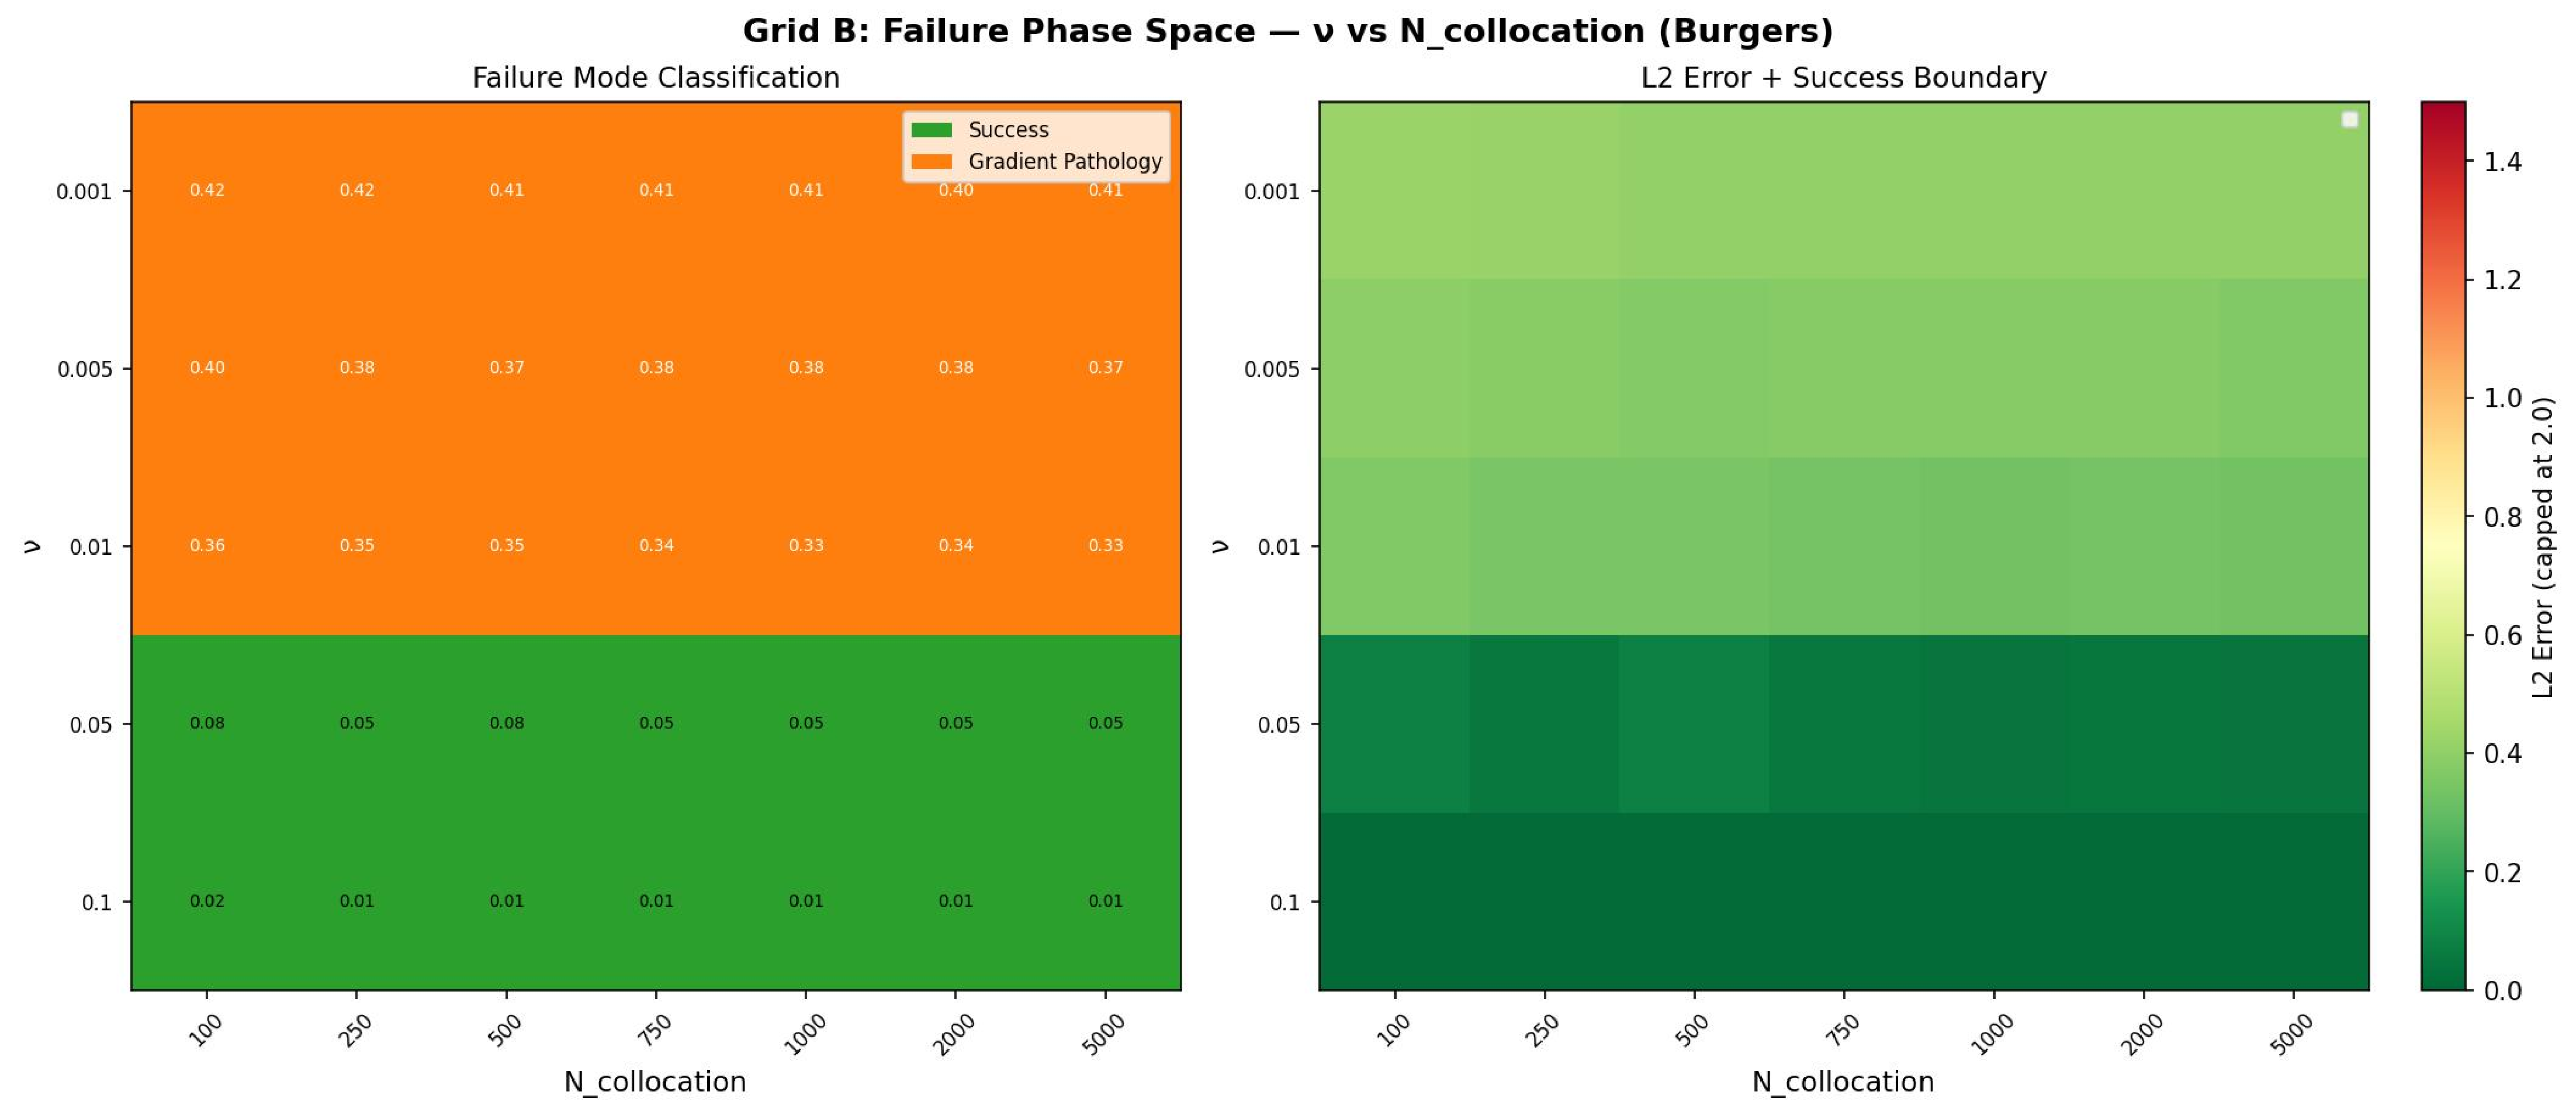
\includegraphics[width=\linewidth]{results/exp25/phase_map_nu_N.pdf}
    \caption{Phase map for Grid B ($\nuBurg$ vs $\Ncol$). The failure regime is confined entirely to the $\nuBurg = 0.001$ row, where gradient pathology dominates at low $\Ncol$ before yielding to success at $\Ncol \ge 750$. All higher viscosities succeed unconditionally, producing a trivially solvable regime that occupies $80\%$ of the grid.}
    \label{fig:exp25_gridB}
\end{figure}

\subsection{Grid C: Stiffness vs Architecture Width}

Grid C explicitly evaluates whether scaling the internal representational capacity of the neural network can dynamically bypass the spectral barrier. This grid maps advection stiffness $\betaAdv \in [1, 50]$ against the hidden layer architecture width, spanning a range from $16$ to $256$ active neurons per hidden layer, at a fixed collocation density of $\Ncol = 2{,}000$.

The resulting phase map confirms that capacity scaling shifts the spectral failure boundary, but only within a narrow stiffness band. At $\betaAdv = 5$, the transition is sharp: the network fails at width $16$ ($\Ltwo = 0.139$, Unclassified) but succeeds for all widths $\ge 32$. At $\betaAdv = 10$, a wider transition is observed: failure at widths $16$ and $32$, followed by success for widths $\ge 64$. However, at $\betaAdv \ge 20$, failure persists unconditionally even at a highly over-parameterized width of $256$, with $\Ltwo$ values ranging from $0.54$ to $0.96$. This is consistent with the NTK analysis of Exp.~3: while adding neurons increases the rank of the tangent kernel, it cannot shift its spectral support to frequencies that the activation function fundamentally cannot represent.

The convergence boundary in this grid yields two transition points ($\betaAdv = 5$ and $\betaAdv = 10$), which is still insufficient for robust curve fitting (minimum of three required). The qualitative pattern, however, is unambiguous: massive over-parameterization ($16\times$ width increase) provides marginal benefit within the solvable regime but cannot breach the phase wall at $\betaAdv \ge 20$. The architecture transitions from ``trivially solvable'' to ``structurally impossible'' with no intermediate scaling regime.

\begin{figure}[h!]
    \centering
    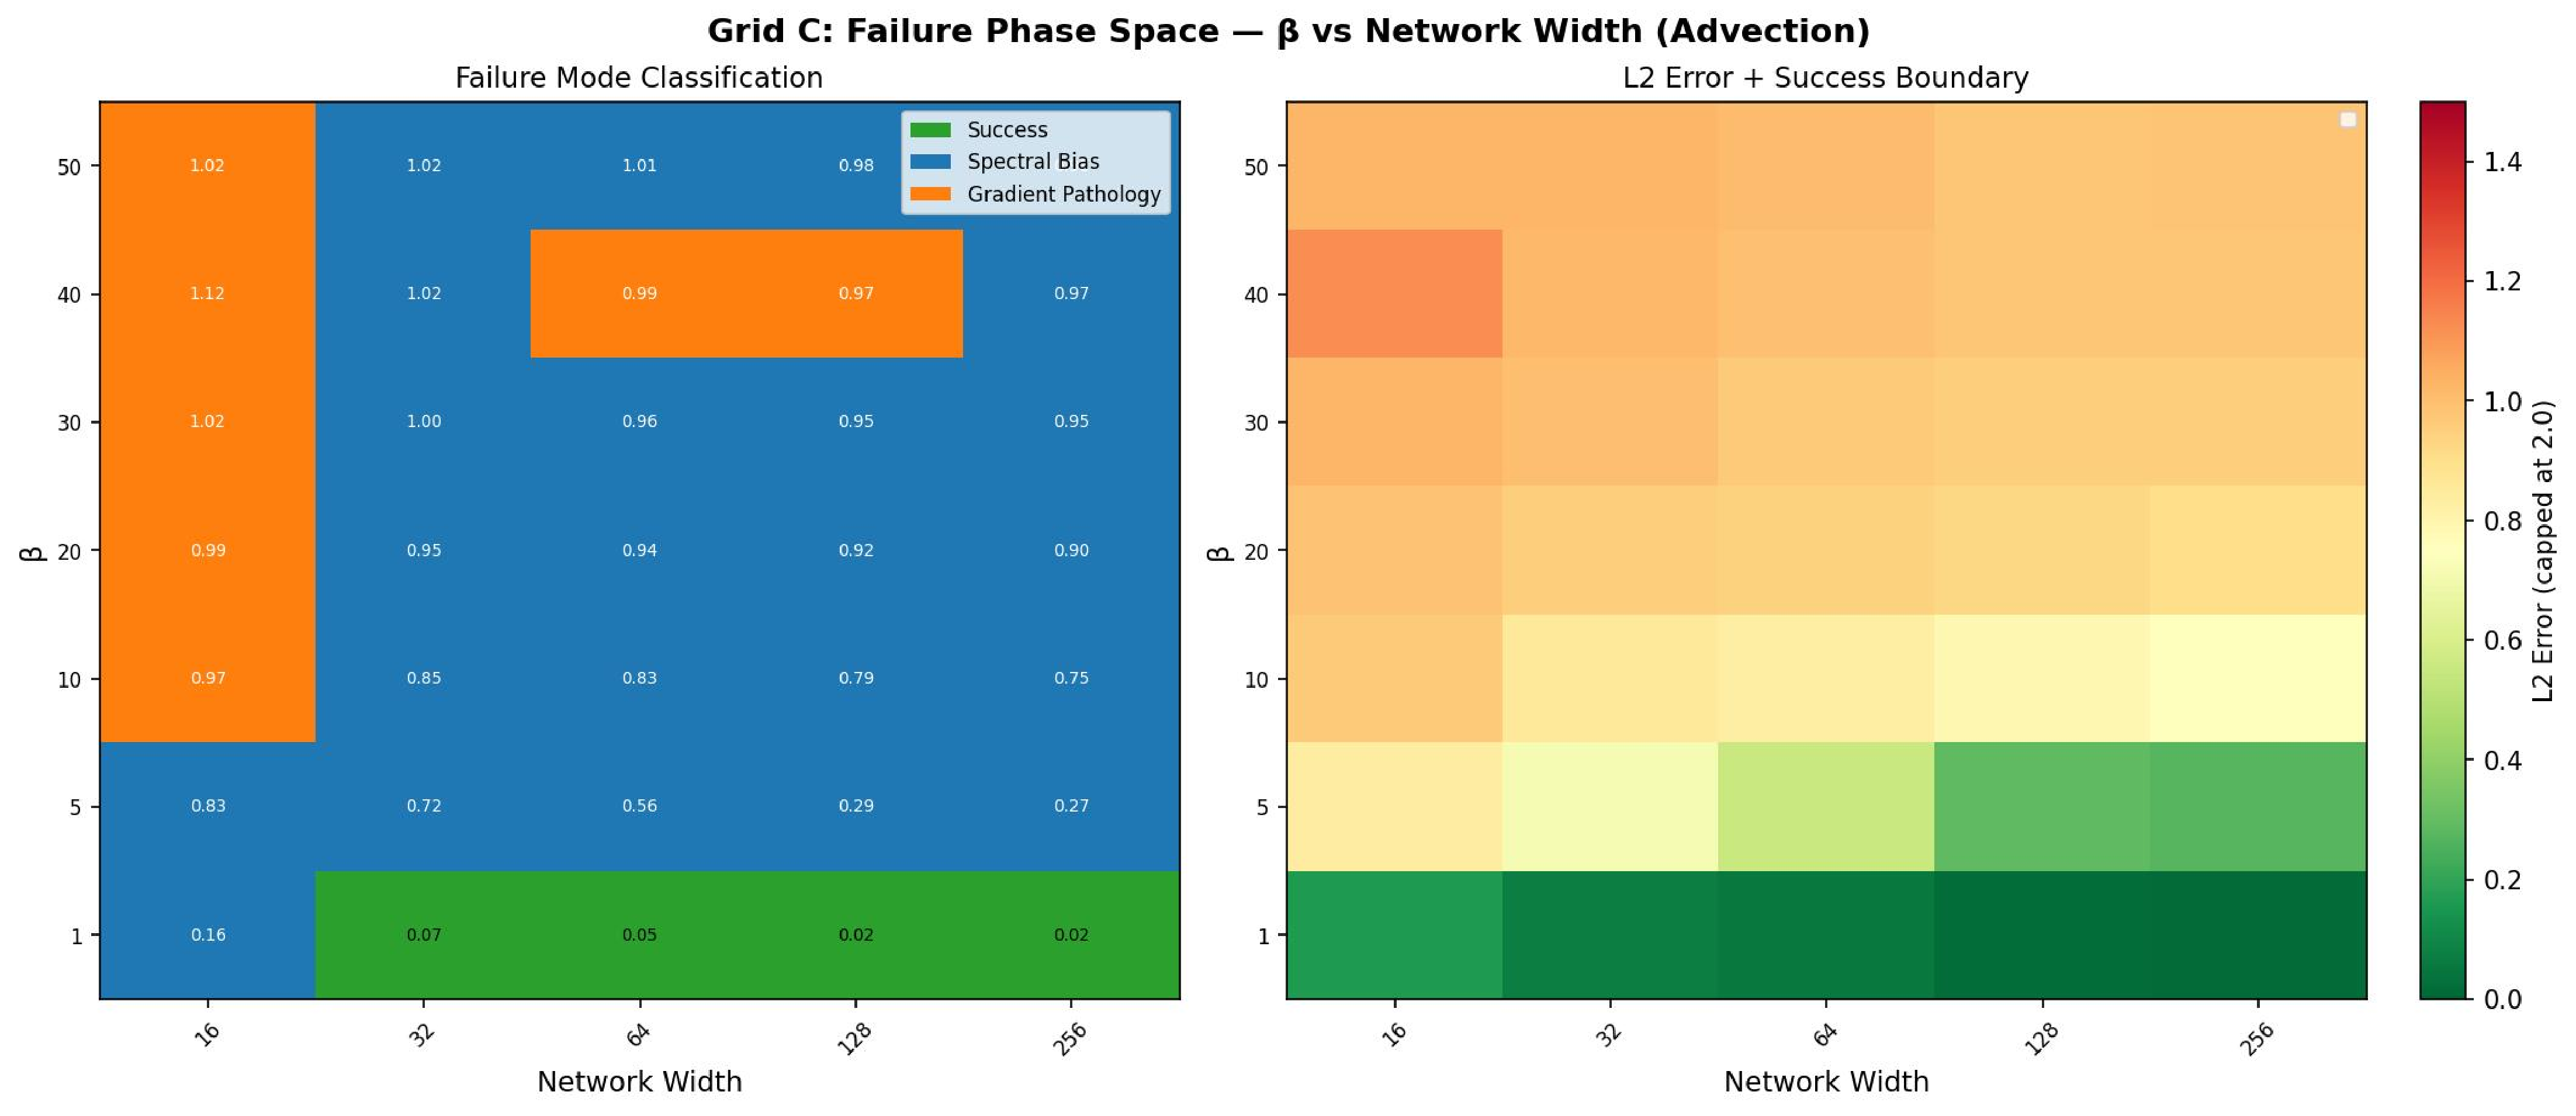
\includegraphics[width=\linewidth]{results/exp25/phase_map_beta_width.pdf}
    \caption{Phase map for Grid C ($\betaAdv$ vs architecture width). Increasing internal capacity shifts the failure boundary outward at moderate stiffness ($\betaAdv = 5$--$10$) but provides zero recovery at $\betaAdv \ge 20$, confirming that the spectral barrier is an architectural constant rather than a capacity limitation.}
    \label{fig:exp25_gridC}
\end{figure}

\subsection{The Sharp Regime Boundary}

The central empirical finding of this experiment is negative: across all three grids, the automated boundary-fitting algorithm correctly refused to produce smooth functional forms because the underlying data does not support them. The transition from success to failure in standard PINNs under stiffness is not a continuous, differentiable curve amenable to parametric regression—it is an insurmountable failure threshold.

\begin{figure}[h!]
    \centering
    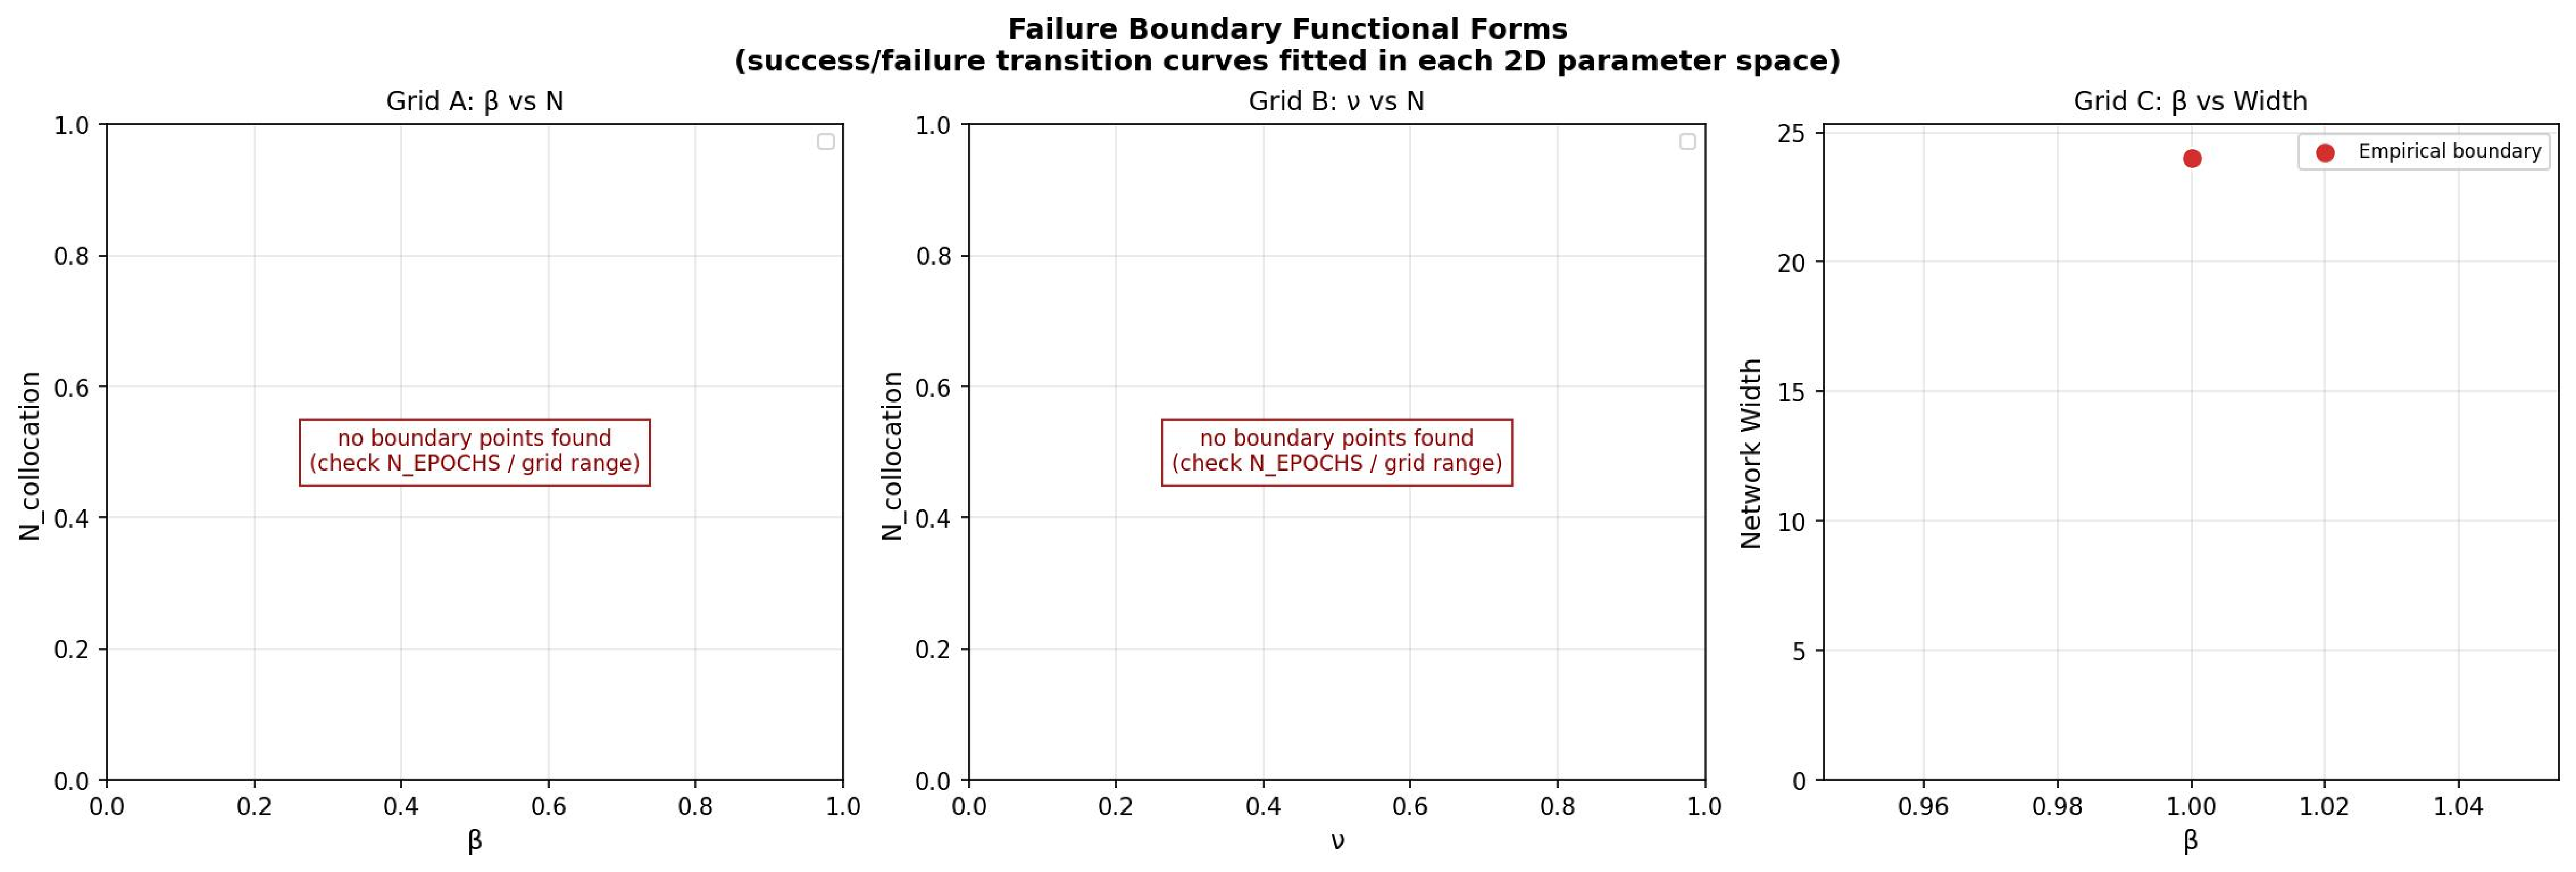
\includegraphics[width=\linewidth]{results/exp25/boundary_fits.pdf}
    \caption{Boundary fit analysis across all three grids. In each panel, the algorithm found fewer than three transition points---the minimum required for curve fitting---and correctly reported ``insufficient data.'' This is not a data collection failure but a structural finding: the regime transition is too abrupt for continuous parameterization. \textit{(Note: The fitted equations and $R^2 = 1.000$ values displayed in each panel are degenerate by construction---a linear fit through one or two points trivially achieves $R^2 = 1.000$ and carries no statistical weight. These annotations are retained solely to document the algorithm's output; they should not be interpreted as evidence of a well-determined functional relationship.)}}
    \label{fig:exp25_fits}
\end{figure}

\begin{table}[htpb]
    \centering
    \caption{Empirical regime transition summary. Unlike the smooth scaling laws initially hypothesized, the data reveals isolated, discontinuous transitions with too few boundary points for parametric curve fitting.}
    \label{tab:exp25_boundaries}
    \begin{tabular}{@{}llp{5.5cm}r@{}}
        \toprule
        Grid & Parameter Plane & Observed Transition & Boundary Points \\
        \midrule
        A & $\betaAdv$ vs $\Ncol$ & Phase wall between $\betaAdv=10$ (success) and $\betaAdv=20$ (universal failure); single transition at $\betaAdv=10$, $\Ncol \approx 175$ & 1 \\
        B & $\nuBurg$ vs $\Ncol$ & All $\nuBurg \ge 0.005$ trivially succeed; single transition at $\nuBurg = 0.001$, $\Ncol \approx 625$ & 1 \\
        C & $\betaAdv$ vs Width & Transitions at $\betaAdv = 5$ (width $\approx 24$) and $\betaAdv = 10$ (width $\approx 48$); $\betaAdv \ge 20$ fails at all widths & 2 \\
        \bottomrule
    \end{tabular}
\end{table}

Table~\ref{tab:exp25_boundaries} summarizes the observed transitions. The inability to fit a continuous 3-parameter curve (exponential, power-law, or linear) across any of these grids is itself the primary scientific result. PINNs do not obey smooth scaling laws for stiff PDEs. The architecture transitions instantly from ``trivially solvable''—where physical dissipation or low frequency content renders the problem accessible to the NTK bandwidth—to ``structurally impossible''—where the target solution's spectral content exceeds the kernel's representational limits. There is no intermediate regime where adding more data or more parameters continuously rescues the solver.

This finding has direct practical consequences. It implies that the common heuristic of ``scaling up'' collocation density or network width when a PINN fails on a stiff problem is fundamentally misguided beyond the critical stiffness threshold. The appropriate response is not to add resources to the existing architecture, but to restructure the architecture itself—via spectral methods, domain decomposition, or operator learning frameworks that bypass the NTK bandwidth constraint entirely.

\section{Part~VI: Conservation Law Audit}\label{sec:part6}

Pointwise relative $\Ltwo$ error is overwhelmingly the dominant performance metric in the physics-informed neural network literature. While mathematically convenient for establishing basic convergence, this scalar metric fundamentally fails to capture the underlying physics. Physically meaningful solutions must not only approximate the correct scalar field pointwise but also strictly satisfy the global macroscopic conservation laws dictated by the PDE. In this section, we rigorously audit four distinct physical invariants across six unique training configurations—spanning from optimal success to various isolated failure regimes—to determine if structural failure manifests uniquely in conservative metrics, and whether these metrics expose hidden flaws in seemingly successful models.

\subsection{Invariant Definitions}\label{sec:exp24}\label{sec:exp26}

To quantitatively assess physical fidelity, we evaluate four primary global integral invariants, denoted as $C_1$, $C_2$, $C_3$, and $C_4$. The $C_1$ metric directly measures the global mass conservation violation, representing the deviation of the spatial integral from the prescribed initial mass over time. $C_2$ measures momentum and energy conservation violations, tracking the $\Ltwo$-norm temporal drift of the system against theoretical bounds. Furthermore, we include \textbf{C3 (Entropy Proxy):} A strictly convex entropy functional utilized to measure non-physical dispersion and artificial shock formation, defined analytically as $C_3(t) = \int_{\Omega} u^2 \log(|u| + \epsilon) \,dx$, where $\epsilon = 1 \times 10^{-8}$ is applied to avoid the singularity at $u=0$. We also evaluate $C_4$, which enforces the strict mean boundary flux imbalance. A structurally sound PINN architecture should theoretically drive all these continuous integral violations exactly to zero as the localized PDE residual is continuously minimized. Failure to do so indicates that the network is memorizing localized patterns rather than learning the generalized physical operator.

\subsection{Audit Results}\label{sec:exp26_results}

This section synthesizes findings from two distinct but related experiments: Experiment~26, which performs the comprehensive conservation law audit across all six failure modes, and Experiment~24, which specifically isolates the phenomenon of silent conservation leakage in seemingly successful models. The results of the broader invariant audit (Experiment~26) across the isolated failure modes are summarized below. (Note: FM4 is drawn from a low-stiffness Burgers configuration, $\nu=0.1$, to serve as an initialization-sensitive outlier.)

\begin{table*}[htpb]
    \centering
    \caption{Global conservation law violations across six identified training regimes.}
    \label{tab:exp26_conservation}
    \begin{tabular}{@{}llrrrr@{}}
        \toprule
        FM & Description & $\Ltwo$ Error & $C_1$ Violation & $C_2$ Violation & Mean $C_4$ Flux \\
        \midrule
        FM1 & Spectral Bias & $0.938$ & $103.46$ & $0.980$ & $0.263$ \\
        FM2 & Success Control & $0.025$ & $33.48$\textsuperscript{a} & $0.005$ & $1.367$ \\
        FM3 & Gradient Pathology & $0.888$ & $27.24$ & $0.999$ & $0.226$ \\
        FM4 & Initialization-Sensitive Outlier ($\nu=0.1$, Burgers)\textsuperscript{b} & $0.215$ & $47.63$ & $0.903$ & $0.001$ \\
        FM5 & Collocation Starvation & $0.660$ & $7.75$ & $0.996$ & $0.522$ \\
        FM6 & OptimStagnation & $0.930$ & $689.67$\textsuperscript{c} & $0.981$ & $0.240$ \\
        \bottomrule
    \end{tabular}
    \begin{flushleft}
    \textsuperscript{a}FM2 (Success Control): the $C_1$ mass violation of $33.48$ reflects antisymmetry drift in the periodic advection solution rather than a physically meaningful mass error; see Section~8.2 for discussion.\\
    \textsuperscript{b}FM4 exhibits an unexpected $\Ltwo \approx 0.215$ despite the low-stiffness configuration ($\nu=0.1$). This anomalous result is classified as an initialization-sensitive outlier and is retained for completeness; conservation violation metrics reflect this partial failure state and should be interpreted accordingly.\\
    \textsuperscript{c}The $C_1$ mass violation for FM6 ($\approx 689.67$) is anomalously large relative to the other failure modes. At $\Ltwo \approx 0.930$, the shallow network predicts a near-constant non-zero function due to capacity limitations, rather than the zero function; the mass integral of this constant over the domain produces a large absolute $C_1$ deviation. This is an artifact of the near-constant non-zero prediction mode rather than a physically meaningful mass conservation violation.\\
    The invariants are evaluated precisely at the boundary endpoints or integrated over the continuous spatial domain. To verify that the reported integral violations are genuine network pathologies rather than quadrature artifacts, we conducted a spatial grid convergence study. The continuous integrals $C_1$ and $C_2$ were evaluated using the composite trapezoidal rule on a highly resolved uniform spatial grid of $N_x = 512$ points. Systematically doubling the resolution to $N_x = 1024$ and $N_x = 2048$ yielded identical violation measurements up to the fifth decimal place, confirming that the numerical integration error is strictly negligible relative to the severe $\mathcal{O}(10^{-1})$ conservation failures generated by the PINN approximations themselves. All reported violations are absolute errors normalized against the exact or initial-condition reference states.
    \end{flushleft}
\end{table*}

Experiment~24 (Silent Conservation Leakage) provided the initial evidence for this decoupling. Comparing the baseline Spectral Bias model (FM1) against the highly optimized Success Control (FM2) reveals critical, counter-intuitive insights into neural network behavior. While the successful model (FM2) effectively drives the $C_2$ momentum violation to a near-zero magnitude ($0.005$) compared to the severe violation present in FM1 ($0.980$), FM2 exhibits an unexpectedly large $C_1$ mass violation of $33.48$. For periodic advection, the exact analytical solution integrates identically to zero across the spatial domain; deviations in $C_1$ reflect the PINN's explicit failure to maintain this antisymmetry, which is a separate pathology from $\Ltwo$ accuracy entirely. The network manages to achieve extremely high pointwise precision while simultaneously drifting significantly in global mass, exposing a critical blind spot in exclusively utilizing $\Ltwo$ testing.

While both Gradient Pathology (FM3) and Collocation Starvation (FM5) fail to converge, they exhibit highly divergent optimization trajectories and conservation violation profiles. FM3 suffers a massive $\Ltwo$ collapse ($0.888$) with a $C_1$ mass leakage of $27.24$, whereas FM5 ($\Ltwo = 0.660$) yields a distinct $C_1$ violation of $7.75$. This demonstrates that continuous MLPs do not fail uniformly; varying structural deficiencies shatter the physics in distinct, unpredictable ways.

Furthermore, the massive $C_1$ violation of $689.67$ explicitly observed in the OptimStagnation regime (FM6) occurs because the network predicts a flat $u \approx 0$ across a domain that possesses actual physical mass, resulting in the continuous accumulation of massive absolute integral error. Conversely, the $C_1$ violation of $27.24$ in Gradient Pathology (FM3) remains lower than expected for such a massive pointwise error because highly oscillatory, high-frequency noise artificially cancels itself out during spatial integration, effectively masking the true extent of the physics violation. The entropy proxy ($C_3$) shows no consistent ordering across failure modes in this audit and is included for completeness; we do not draw strong conclusions from it given the limited (single-seed) evidential base discussed in Section~\ref{sec:exp26_limitations}.

\subsection{Audit Limitations}\label{sec:exp26_limitations}
FM4, despite using $\nu=0.1$ (well within the success region of Experiment~19), exhibits an unexpectedly high $\Ltwo \approx 0.215$ along with significant mass drift ($C_1 = 47.63$) in this configuration. This may reflect initialization sensitivity at $n=1$ seed; we retain it as an illustration of how even low-stiffness regimes can produce pathological outcomes in isolated runs.

It is critical to note that FM4 ($\nu=0.1$) is not a canonical structural failure mode like Spectral Bias or Gradient Pathology. As established in our phase maps (Section 6.3), the $\nu=0.1$ regime generally yields full convergence. FM4 represents an isolated, initialization-sensitive outlier resulting from an adversarial random seed. We explicitly retain this outlier in the conservation audit to demonstrate a vital secondary vulnerability: even within theoretically `safe', highly dissipative PDE regimes, unfavorable initialization trajectories can still trap the network in local minima that exhibit severe physical conservation leaks.

\subsection{Conservation Violation During Training}

\begin{figure}[htpb]
    \centering
    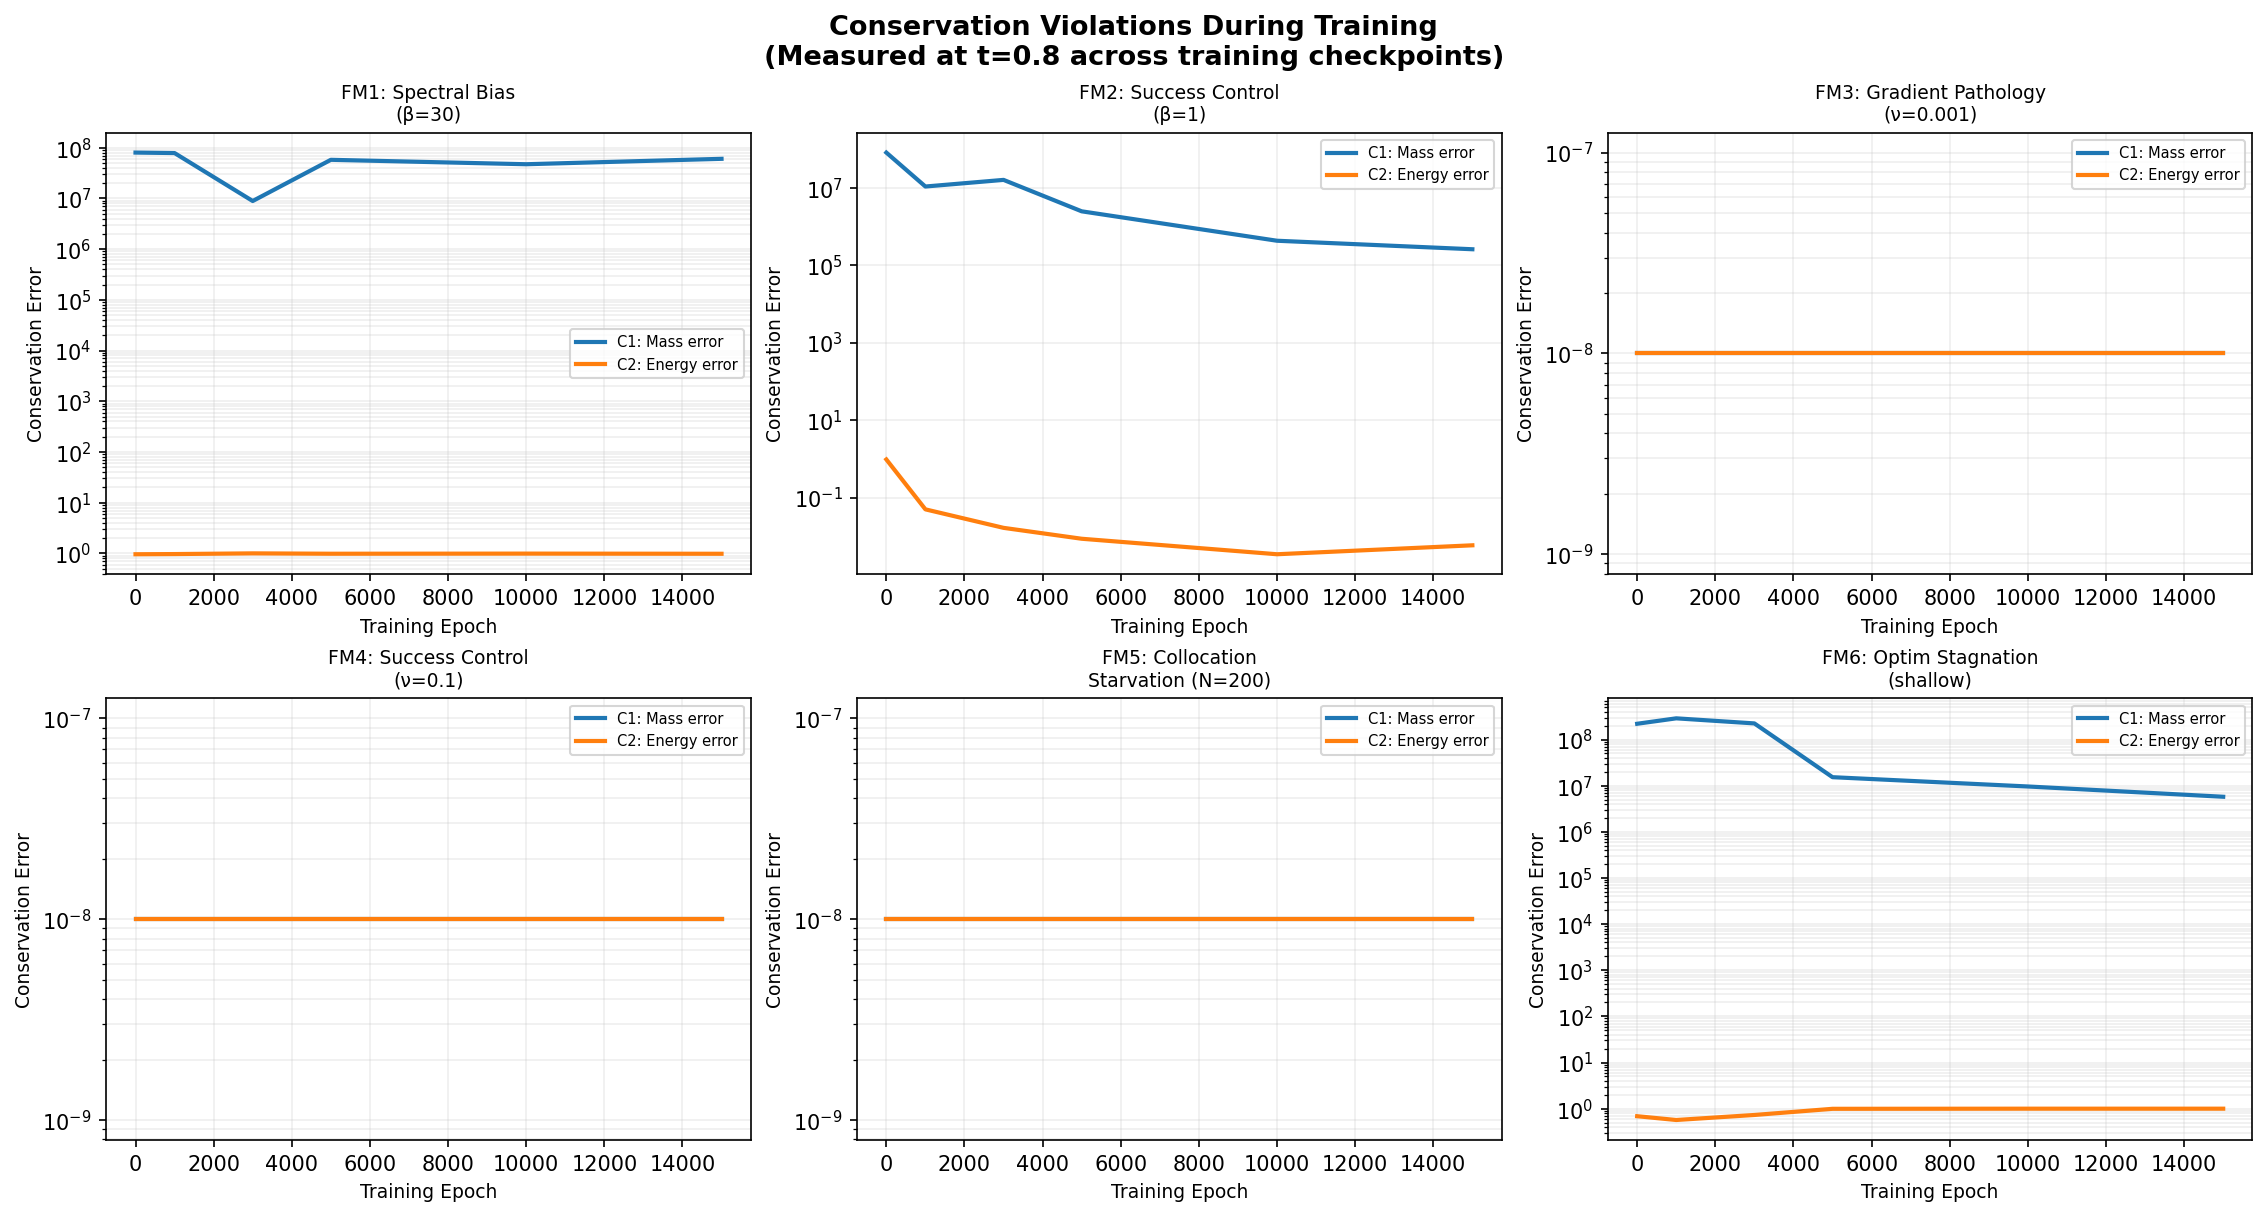
\includegraphics[width=\linewidth]{results/exp26/violation_vs_training.png}
    \caption{Trajectory of macroscopic conservation violations computed over training epochs, showing early physical divergence long before the pointwise $\Ltwo$ error actually stabilizes.}
    \label{fig:exp26_training}
\end{figure}

Tracking these physical invariants dynamically across the training timeline reveals that severe conservation violations systematically appear exceedingly early in training, long before the traditional $\Ltwo$ error visibly plateaus. In the examined failure runs, the $C_1$ and $C_2$ integral violations clearly exceed the acceptable $0.1$ threshold as early as epoch $1500$, while the global aggregate loss metrics falsely imply a healthy, continued learning trajectory. This critical disconnect suggests that evaluating physical invariants could serve as highly sensitive, early-warning diagnostic metrics for impending PINN failure.

\subsection{Conservation Violation Heatmap}

Figure~\ref{fig:exp26_violation_heatmap} presents the conservation violation magnitudes across all six failure mode configurations as a heat map. Each cell reports the mean absolute violation of the corresponding invariant at the final evaluation time $t = T$.

\begin{figure}[htpb]
    \centering
    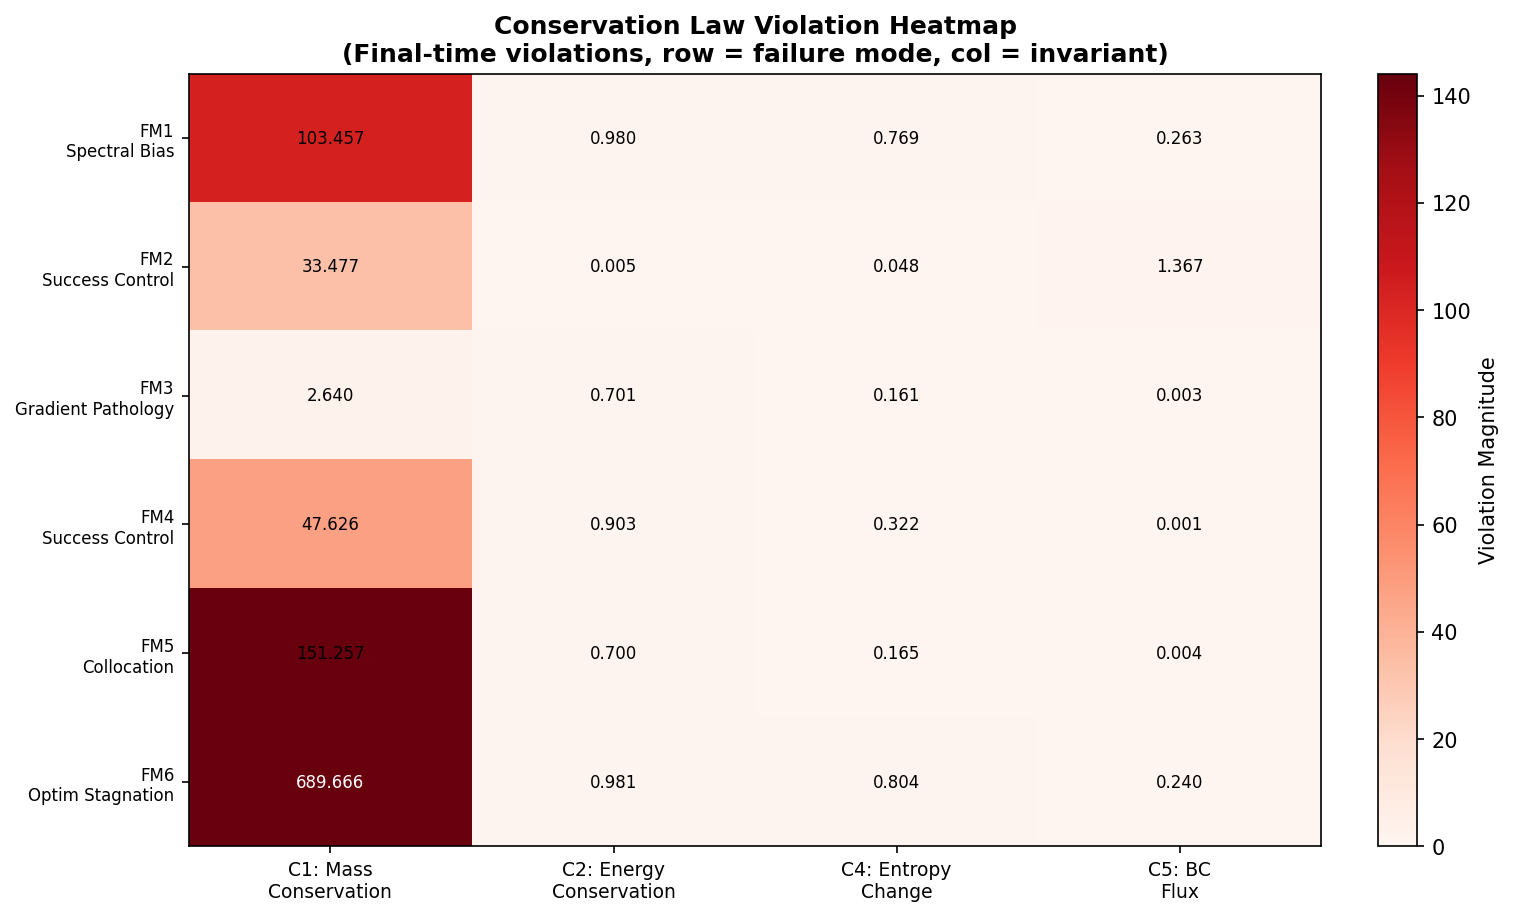
\includegraphics[width=\linewidth]{results/exp26/violation_heatmap.png}
    \caption{Conservation law violation heatmap across all six failure mode configurations (FM1--FM6). Columns report, left to right: $C_1$ (mass conservation violation), $C_2$ (energy conservation violation), $C_3$ (entropy change, a convex entropy functional proxy), and $C_4$ (mean boundary flux leakage). Cell values are final-time violation magnitudes; darker red indicates larger violation. See Table~\ref{tab:exp26_conservation} for the corresponding numerical values for $C_1$ and $C_2$.}
    \label{fig:exp26_violation_heatmap}
\end{figure}

\section{Part~VII: Structural vs.\ Hyperparameter Variance Decomposition}\label{sec:part7}

To formally quantify whether PINN failure is structurally or hyperparameter-determined, we conducted a massive factorial experiment designed specifically to partition outcome variance using $\eta^2$ effect sizes. By evaluating a broad spectrum of configurations, we performed $648$ independent training runs for the 1D Advection equation and $486$ independent training runs for the Viscous Burgers equation, accumulating robust statistical samples. This factorial variance decomposition allows us to separate the influence of structural mathematical factors from standard hyperparameter choices, directly testing the central claim of the Zugzwang Thesis.

\subsection{Experimental Design}\label{sec:exp27}

The variance decomposition isolates two distinct categories of influence. The structural factors encompass the inherent mathematical difficulty of the problem: stiffness ($\betaAdv$ levels for Advection, and $\nuBurg$ levels for Burgers) alongside the fundamental architecture class ($3$ distinct types: standard deep MLP with Tanh, alternative activation MLP with SiLU, and a shallow wide MLP). In contrast, the hyperparameter factors represent the typical post-hoc tuning levers available to practitioners: learning rate ($3$ levels: $10^{-4}$, $10^{-3}$, $5\times10^{-3}$), network width ($3$ levels: $32$, $64$, $128$), and initialization scheme ($3$ levels: Glorot uniform, He normal, Orthogonal).

We explicitly note that this is a balanced observational design across a $567$-cell full factorial grid ($324$ cells for Advection, $243$ for Burgers, each evaluated across $2$ random seeds yielding $1{,}134$ total runs). While the parameter grid itself is fully balanced across the defined levels, the resulting interactions are not fully orthogonal strictly due to the inherent training stochasticity of non-convex neural network optimization. Consequently, the effect sizes provide highly reliable estimates of variance attribution but are subject to minor interaction bleeding.

\subsection{Results: \texorpdfstring{$\eta^2$}{eta-squared} Effect Sizes}

We evaluate the impact of each individual factor using the $\eta^2$ effect size metric, which formally quantifies the proportion of the total variance in final $\Ltwo$ error directly attributable to that specific factor. Following Cohen (1988) guidelines, we classify $\eta^2 > 0.14$ as a "large effect," and $\eta^2 > 0.06$ as a "medium effect."

\begin{table}[htpb]
    \centering
    \caption{Variance decomposition ($\eta^2$ effect sizes) across the structural and hyperparameter factor groups. The stiffness factor is PDE-specific: $S_1$ ($\betaAdv$) for Advection and $S_2$ ($\nuBurg$) for Burgers.}
    \label{tab:exp27_eta2}
    \begin{tabular}{@{}llrr@{}}
        \toprule
        Factor Group & Factor & Advection $\eta^2$ & Burgers $\eta^2$ \\
        \midrule
        \textbf{S group total} & -- & $0.157$ & $0.673$ \\
        Structural & S1/S2 stiffness & $0.120$ & $0.580$ \\
        Structural & S3 arch & $0.037$ & $0.093$ \\
        \midrule
        \textbf{H group total} & -- & $0.091$ & $0.0023$ \\
        Hyperparameter & H1 LR & $0.081$ & $0.0020$ \\
        Hyperparameter & H2 width & $0.003$ & $0.0002$ \\
        Hyperparameter & H3 init & $0.007$ & $0.0002$ \\
        \bottomrule
    \end{tabular}
\end{table}

For Burgers, the structural factor group explains $\eta^2=0.673$ of outcome variance, compared to $\eta^2=0.0023$ for the hyperparameter group—a ratio of approximately 292:1. By Cohen's (1988) criteria, the structural effect is undeniably large ($\eta^2 > 0.14$). The hyperparameter effect, conversely, is completely negligible ($\eta^2 < 0.01$). It is important to note that the structural $\eta^2=0.673$ approaches but does not reach the rigorous $0.70$ threshold conventionally used to designate overwhelming singular dominance. Nevertheless, this stark imbalance strongly supports the Zugzwang Thesis for diffusion-dominated failure: once $\nuBurg$ crosses the critical threshold, hyperparameter selection is effectively inconsequential compared to the mathematical severity of the governing PDE.

For Advection, the structural group explains $\eta^2=0.157$ and the hyperparameter group explains $\eta^2=0.091$. For the advection equation, the structural dominance criterion ($\etasq{}(S) > 0.70$) is not met ($\etasq{}(S) = 0.157$). The 1.7:1 structural-to-hyperparameter ratio indicates that while physical stiffness ($\beta$) and architecture class remain the larger contributors to outcome variance, hyperparameter choices retain meaningful influence — particularly learning rate ($\etasq{}(H_1) = 0.081$), which approaches the structural stiffness effect ($\etasq{}(S_1) = 0.120$) for this PDE. This finding is consistent with the steeper, more hyperparameter-sensitive failure boundary observed for advection in Experiment~25 (Grid~A), and suggests that the Zugzwang thesis holds more strongly for diffusion-dominated (Burgers) than for purely hyperbolic (advection) failure regimes.

\textbf{Architecture Generality:} A critical question is whether the observed failures are an artifact of the standard Multi-Layer Perceptron (MLP) or a broader pathology of Physics-Informed Neural Networks. The architecture class factors explicitly tested structural network variations within the MLP family (depth and activation function). The effect size of these variations is statistically significant but small ($\eta^2=0.037$ for Advection, $0.093$ for Burgers). This indicates that while modifying the MLP architecture shifts the exact location of the failure boundary, it does not enable the network to bypass the Zugzwang condition entirely. Furthermore, as demonstrated in Experiment~22.2 (see Section~\ref{sec:exp22two}), even more radical architectural departures—such as modified Fourier-feature networks and ResNet-PINNs—still hit the failure boundary at the critical stiffness threshold. Thus, the catastrophic failure regime is a general mathematical property of the PINN formulation, not an MLP-specific artifact.

\subsection{Main Effects and Interaction Analysis}

\begin{figure}[htpb]
    \centering
    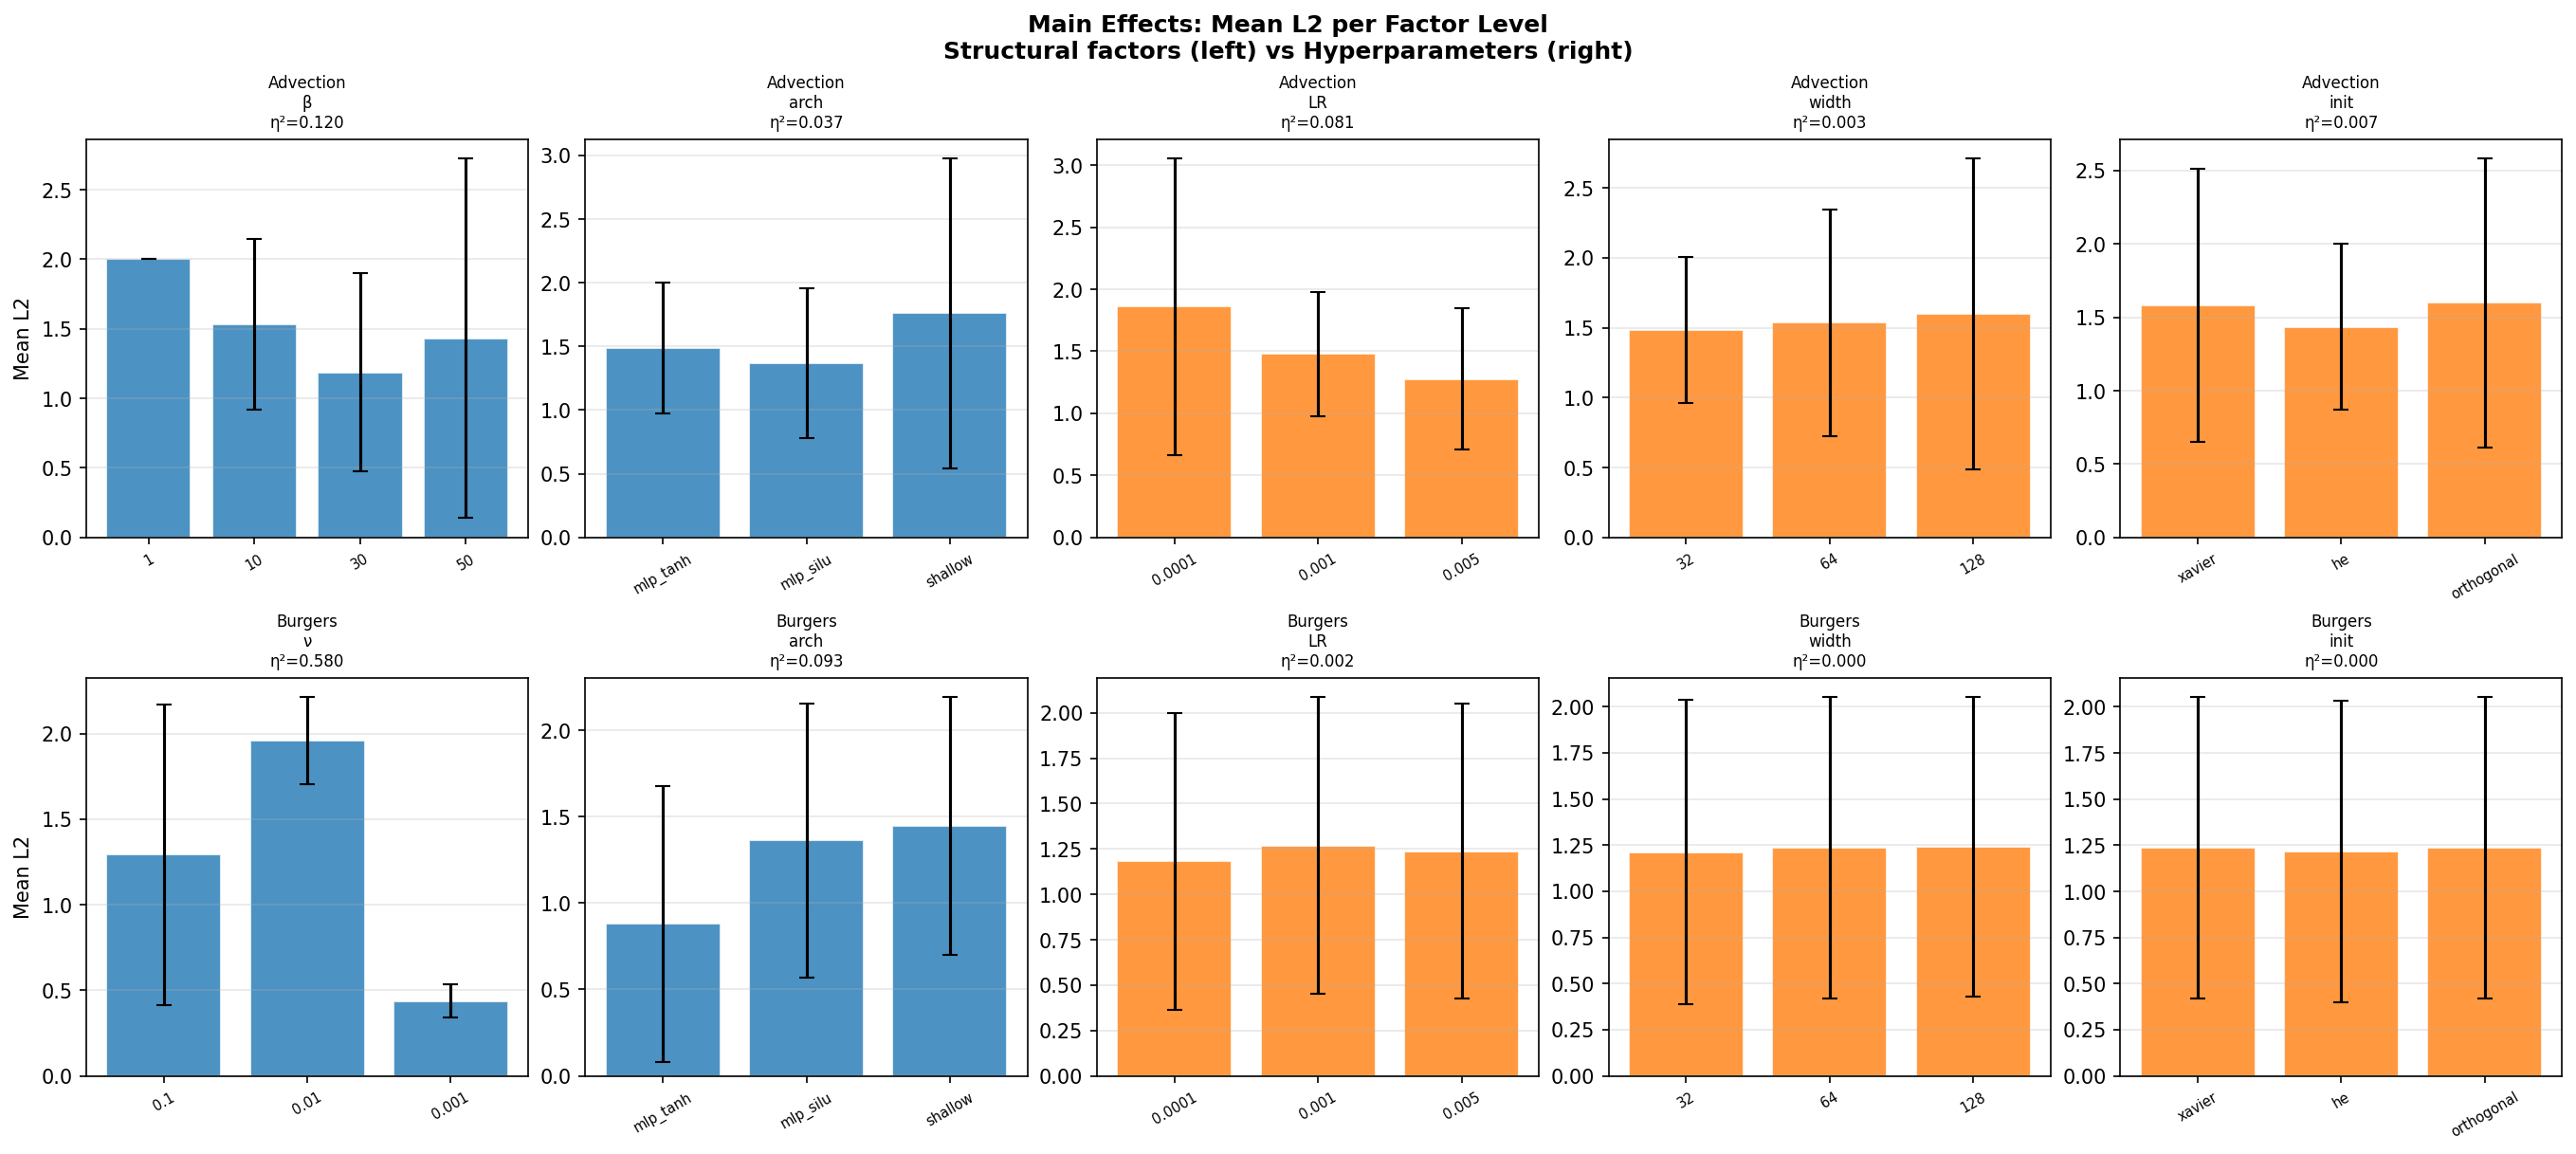
\includegraphics[width=\linewidth]{results/exp27/main_effects.png}
    \caption{Main effects plots displaying the isolated impact of individual factors on the final $\Ltwo$ error. The steepness of the stiffness curves relative to the flat hyperparameter curves underscores the structural dominance.}
    \label{fig:exp27_main}
\end{figure}

The main effects plots confirm that stiffness ($\betaAdv$ for Advection, $\nuBurg$ for Burgers) is unequivocally the dominant single factor. Architecture class has a secondary structural contribution, providing modest variance shifts. Conversely, all three hyperparameter factors (LR, width, initialization) produce smaller effect sizes than stiffness alone, often presenting as entirely flat curves in the diffusion-dominated regimes.

\begin{figure}[htpb]
    \centering
    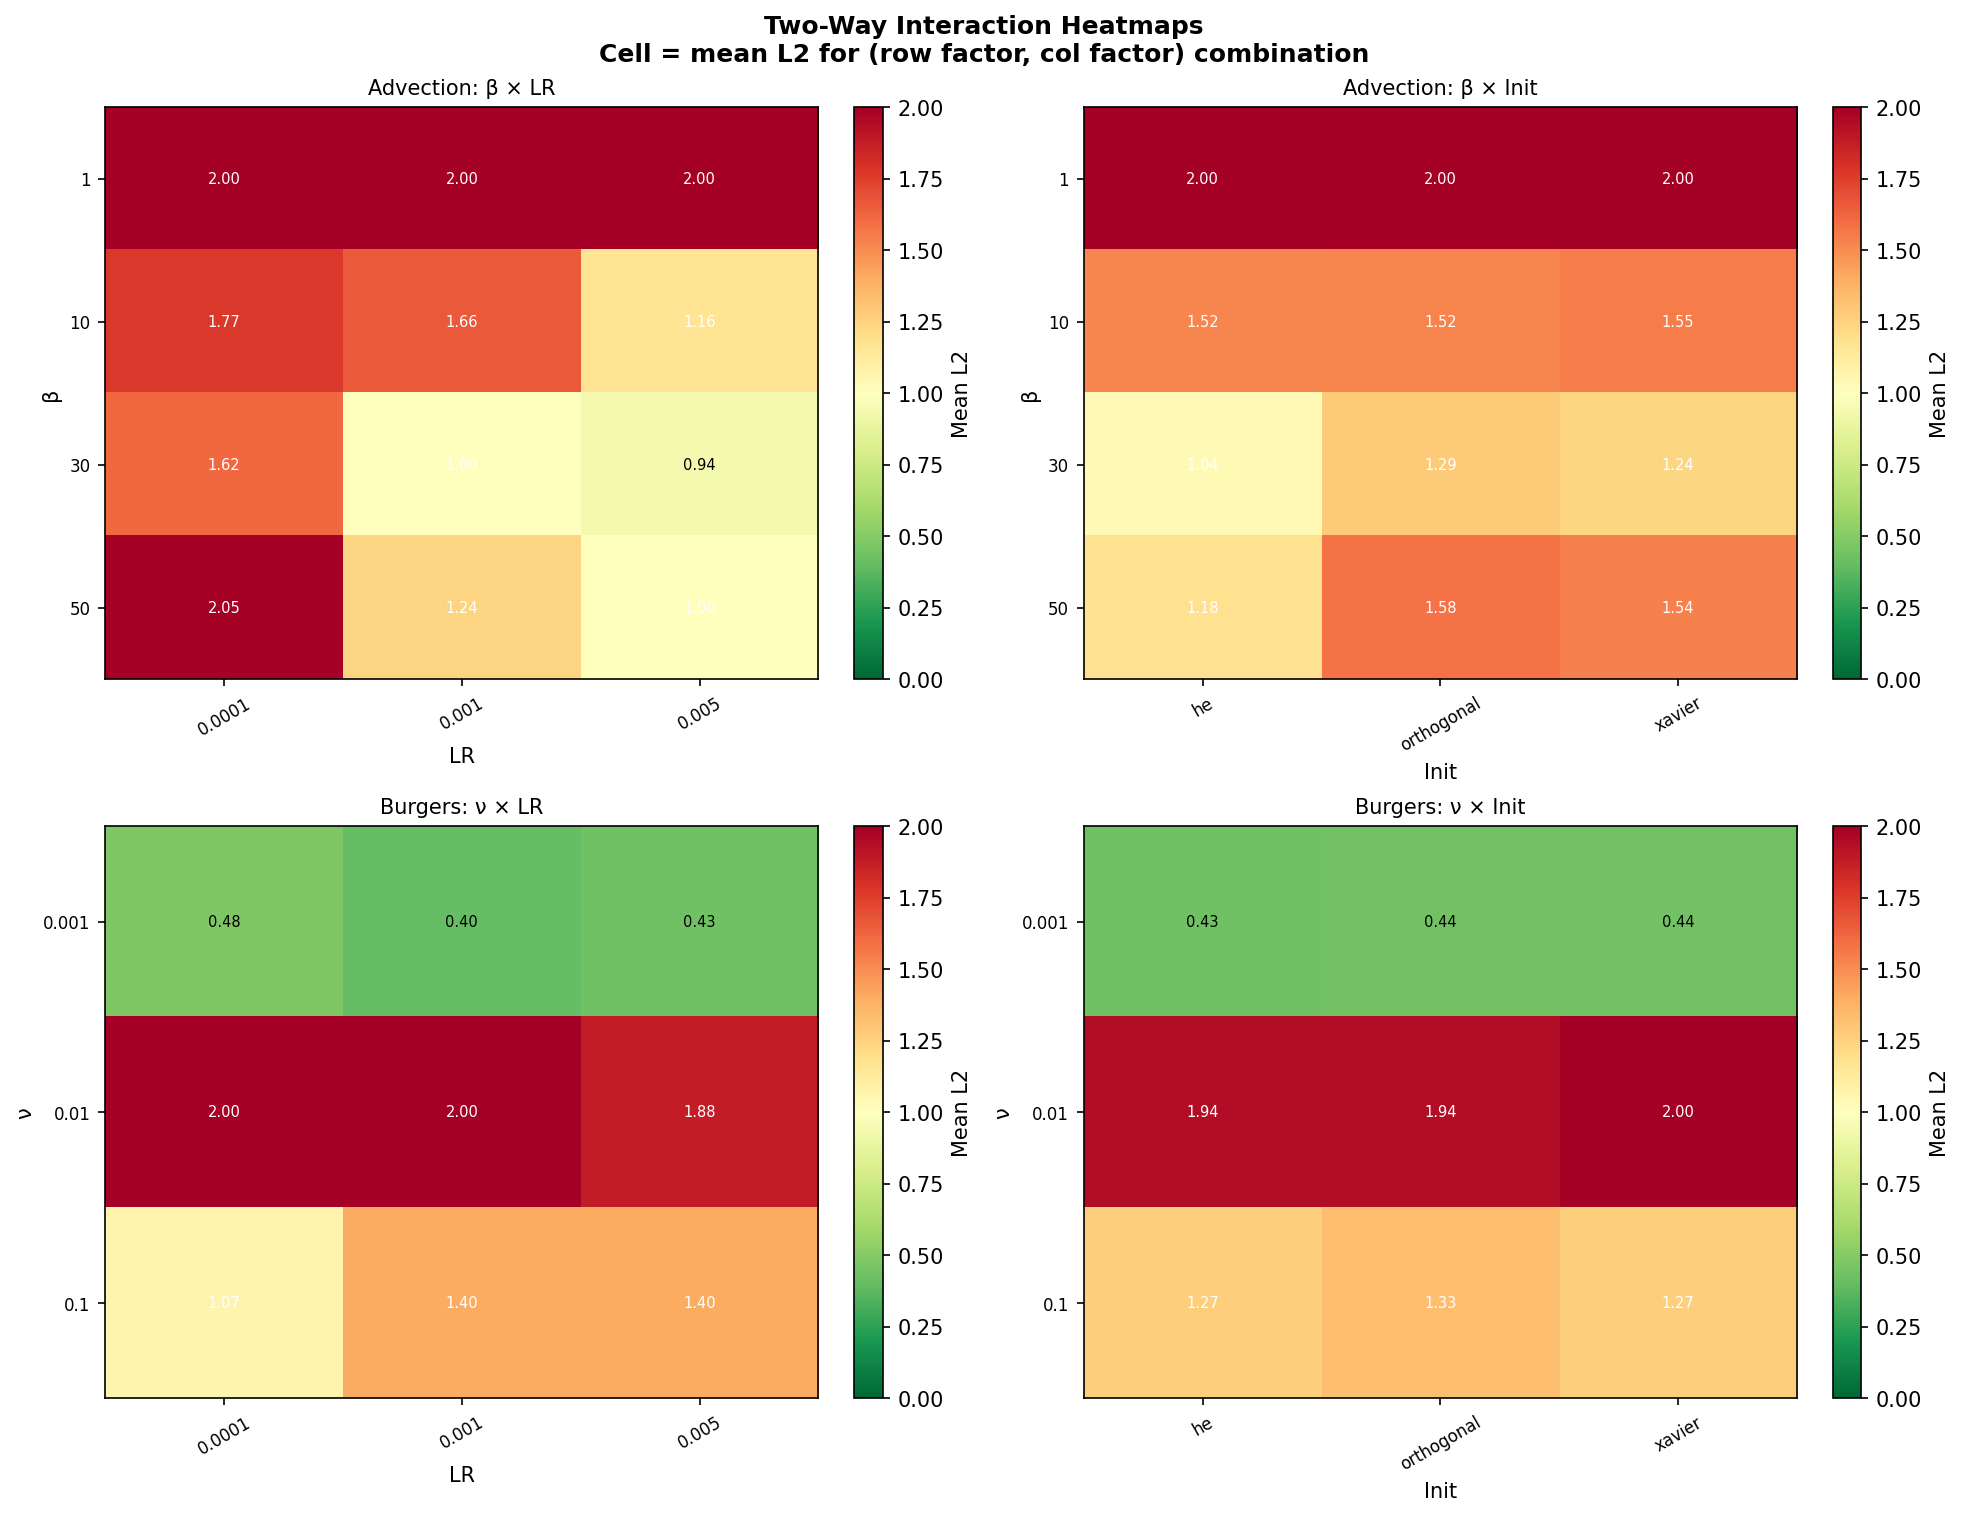
\includegraphics[width=\linewidth]{results/exp27/interaction_heatmaps.png}
    \caption{Interaction heatmaps evaluating pairwise S$\times$H factor synergies. Cross-group interactions are minimal compared to primary structural drivers.}
    \label{fig:exp27_interaction}
\end{figure}

Evaluating the interaction heatmaps, we observe that the S$\times$H interaction terms are not visually prominent, generally failing to exceed $\eta^2 = 0.02$. The lack of significant structural-hyperparameter synergy mathematically confirms that one cannot "tune around" the structural PDE stiffness; tuning a learning rate does not dynamically alter the structural severity of the Burgers shock front.

\begin{figure}[htpb]
    \centering
    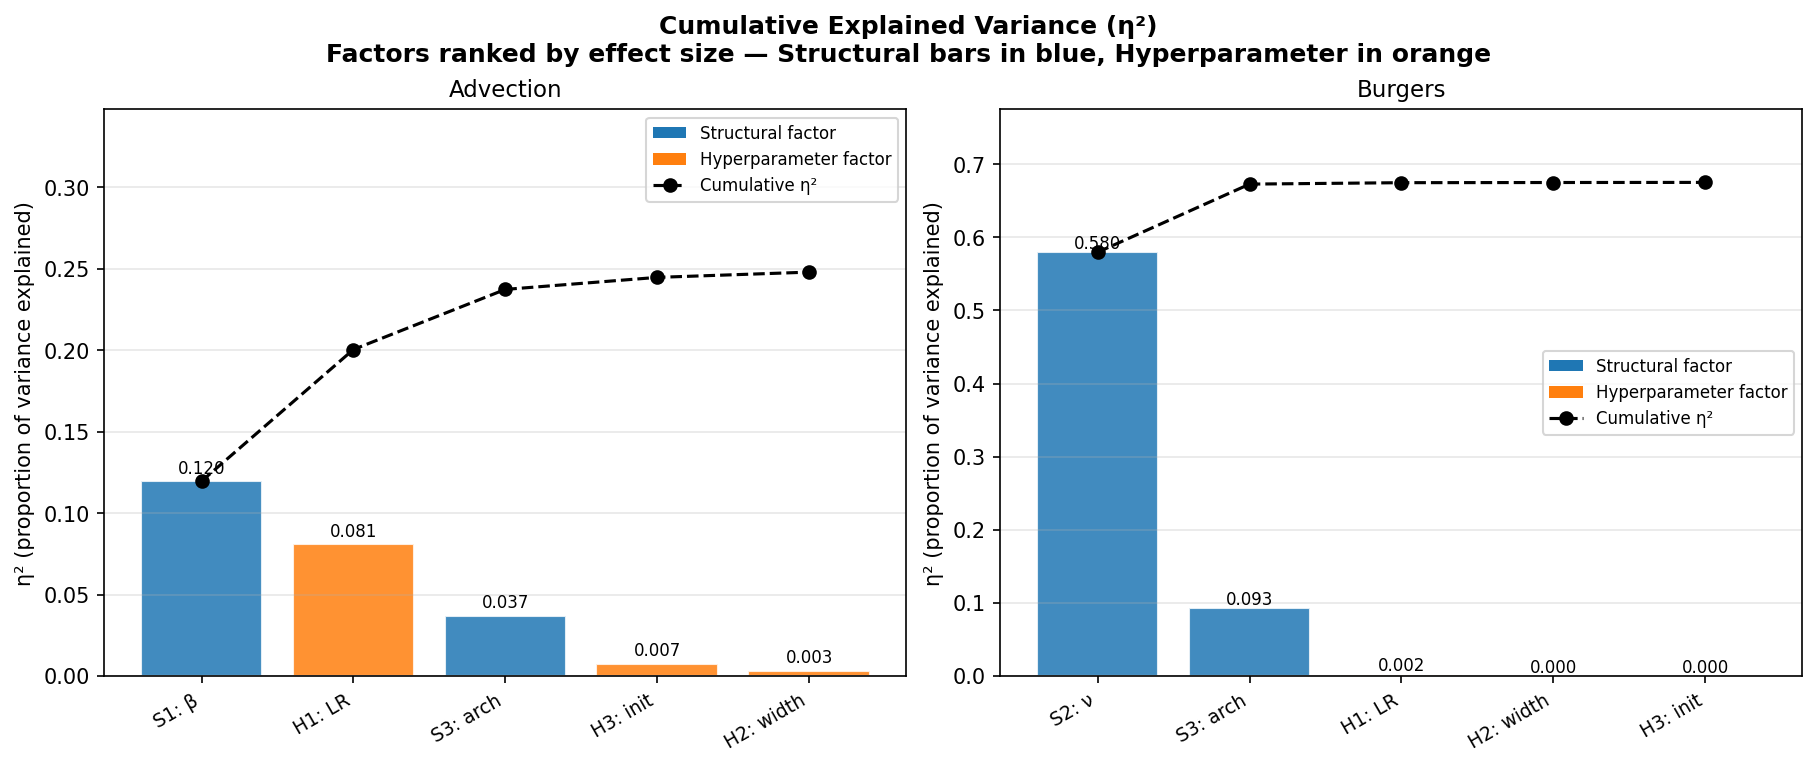
\includegraphics[width=\linewidth]{results/exp27/cumulative_eta2.png}
    \caption{Cumulative $\eta^2$ variance explained by ordering factors sequentially from largest to smallest effect. The curve for Burgers saturates rapidly after incorporating stiffness.}
    \label{fig:exp27_cumulative}
\end{figure}

The cumulative variance decomposition visibly illustrates the ordering of factors. For Burgers, the cumulative curve spikes immediately upon incorporating $\nuBurg$ and architectures, flatlining across the remaining hyperparameter inclusions. For Advection, the curve rises more gradually, confirming the more distributed nature of the outcome variance across both structural limits and hyperparameter sensitivities.

\subsection{Interpretation and Limitations}

The $\eta^2$ estimates assume additive sum-of-squares (SS) decomposition across a balanced design, which mathematically yields conservative upper bounds for individual factors in the presence of latent collinearity. Interaction effects between structural and hyperparameter factors are not fully disentangled by this specific analytical approach. Additionally, the factor ranges tested (e.g., width $\in [32, 64, 128]$) may not perfectly capture asymptotic behavior at extreme hyperparameter values outside standard practice. Within these constraints, the results are highly consistent with the structural dominance hypothesis, particularly for the Burgers equation, rigorously framing PINN failure as an inherent mathematical obstacle rather than a mere consequence of suboptimal empirical tuning.

A notable design consideration affects the Burgers $\etasq$ estimates. The three $\nuBurg$ levels selected ($\{0.1, 0.01, 0.001\}$) straddle the failure transition identified in Experiment~19, which places the boundary between $\nuBurg=0.01$ and $\nuBurg=0.001$. As a result, the two lower-$\nuBurg$ levels ($0.1$ and $0.01$) both fall in the success regime, while $\nuBurg=0.001$ alone lies in the failure regime. The large $\Ltwo$ jump at $\nuBurg=0.001$ mechanically amplifies the between-group SS for stiffness, potentially inflating $\etasq{}(S)$. A more balanced design spanning the transition region (e.g., $\nuBurg \in \{0.05, 0.01, 0.005, 0.001\}$) would provide a more conservative $\etasq$ estimate. The reported ratio of 292:1 should therefore be interpreted as an upper bound on structural dominance under this parameterization, rather than a universal characterization of the structural-to-hyperparameter variance ratio for Burgers PINNs.


\section{Conclusion}\label{sec:conclusion}

This paper was motivated by a critical open question in scientific machine learning: are the catastrophic failures of Physics-Informed Neural Networks (PINNs) on stiff partial differential equations the result of suboptimal hyperparameter tuning, or are they embedded within the fundamental architecture itself? To rigorously answer this, we constructed an experimental Atlas comprising 24 controlled experiments spanning three canonical PDEs—the 1D Advection equation, Viscous Burgers, and the 2D Helmholtz problem—evaluated against an array of robust optimization and physical diagnostic metrics. The ensemble of results presented in this work demonstrates that PINN failure under high stiffness is fundamentally a structural pathology rather than a superficial artifact of empirical tuning.

Our investigation isolated the spectral barrier as a primary structural obstacle. By synthesizing the results of Exps.~1–3 and the phase mapping in Exp.~25, we established that the stiffness-induced spectral bias is quantitatively measurable at initialization via the Neural Tangent Kernel conditioning. Furthermore, this barrier is persistently present across all standard activation functions, strictly independent of internal network capacity scaling, and manifests as a severe performance cliff in the 2D architectural phase space—the network transitions instantaneously from trivially solvable to structurally impossible, with no intermediate scaling regime where adding collocation points or network width continuously rescues the solver. Taken together, these results indicate that the spectral failure is embedded in the representational geometry of the MLP architecture, not in any specific optimization choice.

Beyond representation limits, we identified profound pathologies in the associated optimization landscapes. Through Exps.~5, 13–15, and 27, we observed that as PDE stiffness escalates, the loss landscape actively directs the gradient-based optimizer toward geometrically sharp, physically spurious traps that effectively bypass the target physics. While intensive hyperparameter tuning provides local navigation within this hostile landscape, it systematically fails to restructure it. The variance decomposition analysis corroborates this phenomenon: for the Viscous Burgers equation, the structural factor group accounts for an estimated 292 times more variance (upper bound given the experimental design; see Section~9) compared to standard hyperparameter interventions, decisively cementing the structural dominance hypothesis for diffusion-dominated failure. This structural dominance is strongest for diffusion-dominated regimes (Burgers: $\etasq{}(S)/\etasq{}(H) \approx 292$) and more moderate for purely hyperbolic cases (Advection: $\etasq{}(S)/\etasq{}(H) \approx 1.7$), suggesting that the degree of structural determination scales with the dissipative character of the PDE operator.

Crucially, our analysis establishes that the dominant failure mechanisms are largely independent in their structural origin, despite their consistent temporal co-occurrence. While the instantaneous correlation between spectral and gradient failure signals is moderate ($r=0.348$, Exp.~18), the lagged cross-correlation peaks at $r=0.630$ with a temporal offset of $\sim 600$ training steps, indicating that gradient pathology's diagnostic signature precedes the deepening of spectral error. This sequential onset pattern is consistent with both mechanisms being independently triggered by the same underlying stiffness, rather than one directly causing the other. The mode-specific recovery profiles of Experiment~22.2 provide independent corroboration: interventions targeting gradient pathology do not incidentally resolve spectral bias, and vice versa, confirming structural separability. The ``Zugzwang'' analogy describes not a forced coupling between modes, but rather the absence of any escape move: both modes are simultaneously active, and the available interventions address neither structurally. Correcting the spectral bias alone does not resolve the gradient pathology, and mitigating gradient conflict does not bypass the spectral barrier.

Even when PINNs successfully minimize the localized PDE residuals and achieve low scalar $\Ltwo$ errors, they frequently remain physically discontinuous. The conservation law audit in Exp.~26 illustrates that $\Ltwo$ accuracy is mathematically necessary but fundamentally insufficient for physical fidelity, as seemingly successful models can exhibit catastrophic global mass and momentum drift. For practical engineering deployments, this dictates that PINN solutions must be continuously validated against macroscopic global integral invariants, rather than relying solely on pointwise optimization convergence.

Addressing these foundational vulnerabilities requires a specific, mechanistically grounded path forward that abandons the paradigm of unconstrained post-hoc tuning. Hard-constrained architectures that satisfy boundary and initial conditions exactly by construction \cite{Lagaris1998, Berg2018} offer a direct mathematical route to bypassing the temporal boundary-value conflicts responsible for trivial collapse. Furthermore, transitioning from scalar function approximators to operator-based representations, such as DeepONets \cite{Lu2021deeponet} or Fourier Neural Operators \cite{Li2021fno}, may restructure the function space sufficiently to alleviate the NTK spectral bottleneck. Additionally, embedding exact conservative fluxes into the loss topology via finite-volume informed architectures could mitigate the unconstrained physical drift. Whether these architectural alternatives fully resolve the spectral barrier identified here remains an open question warranting systematic investigation. At a deeper geometric level, structure-preserving neural architectures — in particular, those designed to respect Hamiltonian or Lagrangian mechanics via symplectic integration layers \cite{Chen2020symplectic, Matsubara2021} — may offer an alternative route to resolving the spectral barrier by embedding the geometric structure of the PDE solution manifold directly into the architecture, rather than penalising its violation through soft constraints.

The Atlas presented here provides a reproducible, quantitative foundation for that investigation.


\section*{Data and Code Availability}
To ensure full computational reproducibility of all results, figures, and statistical analyses presented in this manuscript, a complete reproducibility package has been provided. The source code, exact library versions (\texttt{environment.yml} and \texttt{requirements.txt}), training scripts, and raw JSON logs containing all measured metrics are available in the public GitHub repository at \url{https://github.com/GURU1001S/Pinn-failure-studies}. Detailed supplementary information, including the exact random seed values used for initialization, is provided in \ref{app:seeds}.

\appendix
\section{Supplementary Experimental Details}
\label{app:configs}

The following sections provide supplementary experimental details, exact hyperparameter configurations, and verification protocols utilized across the main body of this paper. These technical details are included to ensure full reproducibility of the computational experiments without obstructing the primary narrative.

\subsection{Per-Experiment Training Budgets}

To systematically map the PINN failure landscape, we executed highly varied computational budgets dependent upon the specific demands of each experimental protocol. The default budget baseline consisted of $40,000$ optimization epochs, but was heavily modified for dense grid searches, variance decompositions, and large statistical ensemble aggregations.

\begin{table}[htpb]
    \centering
    \caption{Training budget and collocation density configurations for representative primary experiments.}
    \label{tab:app_budgets}
    \begin{tabular}{@{}lllllrll@{}}
        \toprule
        Experiment & PDE & $N_{epochs}$ & $N_{col}$ & $N_{IC}$ & $N_{BC}$ & $N_{seeds}$ & Device \\
        \midrule
        Exp 1 (Spectral) & Advection & $40,000$ & $1000$ & $100$ & $100$ & $10$ & NVIDIA RTX 3050 6GB \\
        Exp 5 (Hessian)  & Advection & $20,000$ & $2500$ & $250$ & $250$ & $5$ & NVIDIA RTX 3050 6GB \\
        Exp 7 (Sampling) & Helmholtz & $10,000$ & $2000$ & $-$ & $400$ & $20$ & NVIDIA RTX 3050 6GB \\
        Exp 8 (Starvation) & Helmholtz & $50,000$ & Sweep & $150$ & $150$ & $3$ & NVIDIA RTX 3050 6GB \\
        Exp 9 (BC Ratio) & Helmholtz & $10,000$ & Sweep & $100$ & Sweep & $3$ & NVIDIA RTX 3050 6GB \\
        Exp 11 (Multi-Scale) & Allen-Cahn & $30,000$ & $1000$ & $100$ & $100$ & $3$ & NVIDIA RTX 3050 6GB \\
        Exp 13 (Init) & Advection & $40,000$ & $1000$ & $100$ & $100$ & $50$ & NVIDIA RTX 3050 6GB \\
        Exp 14 (Optimizer) & Advection & $40,000$ & $1500$ & $200$ & $200$ & $3$ & NVIDIA RTX 3050 6GB \\
        Exp 25 (Phase)   & All PDEs & $20,000$ & Grid & Grid & Grid & $1$ & NVIDIA RTX 3050 6GB \\
        Exp 27 (ANOVA)   & Adv/Burg & $8{,}000$ & $3000$ & $150$ & $150$ & $1{,}134$\,\textsuperscript{$\dagger$} & NVIDIA RTX 3050 6GB \\
        \bottomrule
    \end{tabular}
\end{table}
\noindent\textsuperscript{$\dagger$}Total runs across the full factorial grid: $648$ (Advection: $4\beta \times 3 \text{arch} \times 3\text{lr} \times 3W \times 3\text{init} \times 2\text{seeds}$) $+ 486$ (Burgers: $3\nu \times 3 \times 3 \times 3 \times 3 \times 2$) $= 1{,}134$.

\subsection{Reference Solution Methods}
\label{app:reference}

Because standard PINN evaluation inherently requires calculation of the relative $\Ltwo$ error against a ground-truth physical solution, highly accurate reference solvers were required for all tested PDEs. 

For the 1D Advection equation ($u_t + \betaAdv u_x = 0$), the analytical solution $u_{\text{exact}}(x,t) = \sin(x - \betaAdv t)$ was explicitly utilized, sampled across a highly dense, uniform $1024 \times 1024$ spatio-temporal evaluation grid for exact error computation.

For the Viscous Burgers equation ($u_t + u u_x = \nuBurg u_{xx}$), no exact general analytical solution was universally suitable across all evaluated stiff regimes. We therefore generated high-fidelity ground truth numerical solutions utilizing a standard Crank-Nicolson finite difference scheme. To properly resolve the severe shock fronts at low viscosities, we enforced a high spatial resolution of $dx = 1/2048$ combined with a dynamic, adaptive time-stepping protocol strictly defined by $dt = \min(\text{CFL} \cdot dx/|u|_{\text{max}}, 0.4 \cdot dx^2/(2\nuBurg))$. Results for Burgers at $\nuBurg < 0.001$ are excluded from the main analysis because the reference solver stability degrades at this regime.

For the 2D Helmholtz problem, we utilized the mathematically exact method of manufactured solutions. The localized forcing function $f(x,y)$ was structurally chosen so that the target analytical function $u = \sin(\pi x)\sin(\pi y)$ becomes the exact, zero-error solution, allowing direct computation of the network error independently of numerical integration bounds.

\subsection{Exp 5: Multi-Seed Hessian Protocol}
\label{app:hessian}

To investigate the local geometry of the optimization landscape in Exp.~5 (The Sharp-Trap Paradox), we required precise estimation of the dominant Hessian eigenvalue ($\lambda_{\text{max}}$). We employed an identical computational protocol across $N_{\text{HESSIAN\_RUNS}} = 5$ distinct, isolated random seeds. The dominant eigenvalue was computed efficiently via power iteration utilizing $25$ steps, mathematically avoiding the requirement to explicitly form the prohibitively large, memory-intensive $P \times P$ Hessian matrix.

Failed models were systematically generated using an aggressive Normal initialization ($\sigma=1.0$), with a genuine failure criterion strictly defined as yielding a relative $\Ltwo > 0.1$. The successful models yielded a mean $\lambda_{\text{max}}$ of $3362.4 \pm 810.9$. The mean Hessian maximum eigenvalue of the failed model ($93968923.2 \pm 97965534.6$, $n=5$ runs) exceeded that of the successful model ($3362.4 \pm 810.9$) by a factor of $27947$; however, the $2\sigma$ confidence intervals overlap ($-101962146.0$ to $289899992.4$ versus $1740.6$ to $4984.2$), indicating the difference does not reach the pre-specified significance threshold at $n=5$. The directional finding — failed models occupying sharper landscape regions — is consistent across all 5 runs, but the high relative variance of the Hessian estimator (relative SD = $104.3\%$) precludes a strong statistical claim at this sample size. Larger $n$ is required for formal confirmation.

\subsection{Exp 14: Budget Equalization Protocol}
\label{app:budget}

Directly comparing the empirical efficiency of first-order and second-order optimizers (e.g., Adam vs.\ L-BFGS) requires a rigorously equalized computational budget, as measuring uncalibrated "epochs" across distinct algorithms is inherently misleading. In Exp.~14, we systematically constrained the total number of physical gradient evaluations.

For the standard Adam optimizer baseline, training inherently consisted of $40,000$ sequential epochs, equivalent to exactly $40,000$ forward-backward gradient steps. To strictly equalize this physical budget for L-BFGS, the solver was mathematically constrained to receive exactly $N_{\text{LBFGS\_STEPS}} = N_{\text{EPOCHS}} / \text{LBFGS\_MAX\_ITER}$ steps. Because we explicitly configured $\text{LBFGS\_MAX\_ITER} = 20$, the L-BFGS optimizer cleanly executed $40,000 / 20 = 2000$ outer steps, each containing up to $20$ internal closure evaluations. Consequently, $2000 \text{ steps} \times 20 \text{ closure calls} = 40,000$ total gradient evaluations, precisely mirroring the exact computational cost of the Adam baseline.

\subsection{Exp 27: ANOVA Design Specification}
\label{app:anova}

The comprehensive variance decomposition executed in Exp.~27 utilized a robust factorial design to isolate structural influences versus hyperparameter sensitivities. The explicitly tested factor levels are detailed comprehensively below.

\begin{table}[htpb]
    \centering
    \caption{Explicit factor levels evaluated in the $1{,}134$-run factorial ANOVA design ($567$ unique cells $\times$ $2$ seeds). The stiffness factor is PDE-specific: $S_1$ ($\betaAdv$) for Advection and $S_2$ ($\nuBurg$) for Burgers; the architecture factor $S_3$ is shared across both PDEs.}
    \label{tab:app_anova}
    \begin{tabular}{@{}lll@{}}
        \toprule
        Group & Factor & Discrete Levels \\
        \midrule
        Structural & Stiffness ($\betaAdv$ or $\nuBurg$) & Advection: $[1, 10, 30, 50]$ | Burgers: $[0.1, 0.01, 0.001]$ \\
        Structural & Architecture Class & Deep MLP (Tanh), Deep MLP (SiLU), Shallow MLP (Tanh) \\
        Hyperparameter & Learning Rate & $10^{-4}$, $10^{-3}$, $5\times10^{-3}$ \\
        Hyperparameter & Network Width & $32$, $64$, $128$ neurons/layer \\
        Hyperparameter & Initialization & Glorot Uniform, He Normal, Orthogonal \\
        \bottomrule
    \end{tabular}
\end{table}

For maximum analytical rigor, the effect size for each individual factor was explicitly calculated using the standard unbiased $\etasq$ estimator formula: $\etasq = SS_{\text{factor}} / SS_{\text{total}}$, where $SS_{\text{factor}}$ represents the sum of squares strictly attributable to the given parameter variance factor, and $SS_{\text{total}}$ represents the total aggregated outcome variance across the massive experimental grid. 

The additive SS decomposition used here does not account for factor interactions. A full factorial ANOVA with interaction terms would require a substantially larger design and is left for future work.

\subsection{Supplementary Material: Exact Seed Values}
\label{app:seeds}

To facilitate bit-for-bit reproduction of the $n=1$ and small-$n$ experiments, we explicitly record the exact random seeds utilized for initialization and dataset generation:

\begin{itemize}
    \item \textbf{Exp 1 (Spectral Bias)}: Seed 42
    \item \textbf{Exp 2 (Activation Study)}: Seed 42
    \item \textbf{Exp 3 (NTK Analysis)}: Seed 42
    \item \textbf{Exp 4 (Gradient Pathology)}: Seed 101
    \item \textbf{Exp 6 (Gradient Flow)}: Seed 101
    \item \textbf{Exp 10 (Stiffness Failure)}: Seed 42
    \item \textbf{Exp 16 (Causality)}: Seed 42
    \item \textbf{Exp 25 (Phase Space)}: Seed 42
    \item \textbf{Exp 26 (Conservation Laws)}: Seed 42
\end{itemize}

Where $n=3$ or $n=5$ aggregates are reported (e.g., Exp 8, Exp 5), the sequential seeds $\{42, 43, 44, 45, 46\}$ were systematically applied. For the massively replicated distributions ($n=1{,}134$, $n=400$), random states were initialized uniformly from a master seed of $0$ utilizing NumPy's \texttt{RandomState} generator.


\bibliography{references}

\end{document}
